

%%%%%%%%%%%%%% Document class
%%%\documentclass[a4paper,BCOR1.5cm,twoside,DIV12]{scrbook}
%\documentclass[a4paper,11pt,oneside,DIV15]{scrbook}
%\documentclass[a4paper,11pt,oneside,DIV15]{scrartcl}

% Sele��o do tipo de monografia e das op��es de formata��o
\documentclass[openright,diss]{deletex}

% um tipo espec�fico de monografia pode ser informado como par�metro opcional:
%\documentclass[tese]{deletex}

% O tipo de monografia pode ser:
% diss 			disserta��o de mestrado
% rp 			relat�rio de pesquisa
% prop-tese 		proposta de tese de doutorado
% plano-doutorado 	plano de curso de doutorado
% dipl-ele 		projeto de diploma��o em Engenharia El�trica
% dipl-ecp		projeto de diploca��o em Engenharia de Computa��o
% estagio		relat�rio de est�gio supervisionado 
% ti			trabalho individual
% pep			plano de estudos e pesquisa
% tese			tese de doutorado
% tc			trabalho de conclus�o de mestrado profissional
% espec			monografia de conclus�o de curso de especializa��o

% � importante notar que estes tipos de monografia foram herdados do estilo
% do II/UFRGS e n�o necessariamente aplicam-se ao DELET/EE/UFRGS. Ou seja,
% embora a classe deletex.cls defina uma opcao para elaborar um PEP, isto nao
% significa que um PEP seja exigido pelo PPGEE.

% monografias em ingl�s devem receber o par�metro `english':
%\documentclass[diss,english]{deletex}

% a op��o `openright' pode ser usada para for�ar in�cios de cap�tulos
% em p�ginas �mpares
% \documentclass[openright]{deletex}

% para gerar uma vers�o somente-frente, basta utilizar a op��o `oneside':
% \documentclass[oneside]{deletex}

% A opcao numbers pode ser usada para gerar refer�ncia num�ricas.
% A opcao sort&compress faz com que referencias do tipo [8,5,3,4] sejam
% convertidas para [3-4,8]
%\documentclass[numbers,sort&compress]{deletex}

% A opcao relnum faz com que a numeracao de figuras, tabelas e equa��es
% seja por cap�tulo.
%\documentclass[relnum]{deletex}


%%%%%%%%%%%%%%%%%%%%%%%%%%%%%%%%%%%%%%%%%%%%%%%%%%%%%%%%%%%%%%%%%%%%%%%%%%%%%%%%%%%%%%%%%%%%%%%%%%%%%%%%
% Preambule
\usepackage[latin1]{inputenc}   % Zeichensatz
\usepackage{graphicx}           % Einbinden von Grafiken
\usepackage{verbatim}
\usepackage{alltt}              % Verbatim-Umgebung mit Steuerbefehlen (z.B. fett, kursiv, ...)
\usepackage{booktabs}           % Paket f�r sch�nere Tabellen
\usepackage{subfigure}
\usepackage{url}
\usepackage{ae}
\usepackage{float}
\usepackage{psfrag}
\usepackage{amsfonts}
\usepackage{amssymb}
\usepackage{amsmath}
\usepackage{pstricks,pst-node,pst-text,pst-3d}
\usepackage{hyperref}   % use for hypertext links, including those to external documents and URLs
%\usepackage[brazil]{babel} %get everything translated properly
%\selectlanguage{brazil}
%\usepackage[numbers]{natbib}
\usepackage{enumerate}
%\usepackage{newclude}

\usepackage{listings}           % Paket, um Listings sch�n einbinden zu k�nnen
\lstloadlanguages{Matlab}
%\usepackage[usenames,dvipsnames]{color}
%\usepackage{thumbpdf}           % Thumbnails f�r Seitenvorschau
%\usepackage{algorithm}
%\usepackage{algorithmicx}
%\usepackage{algpseudocode}
%\usepackage[portuguese,onelanguage,ruled,noline,linesnumbered]{algorithm2e}
%\usepackage[portuguese,ruled,noline]{algorithm2e}

%\usepackage{amsmath}
\usepackage{amsthm}
%\usepackage{amsfonts}
%\usepackage{amssymb}
%\usepackage{thmtools}
%\declaretheoremstyle[,
%bodyfont=\normalfont
%]{mystyle}
%\declaretheorem[name=Exemplo,style=mystyle,numberwithin=chapter]{example}
%\declaretheorem[name=Exemplo,numberwithin=section]{example}
%\usepackage{balance}
%\usepackage{setspace}
%
%\usepackage{multirow}
%\usepackage{rotating}
%
%\usepackage{subfig}
%\usepackage{fancyhdr}
%\usepackage{layout}
%\usepackage{chngpage}
%\usepackage{colortbl}
%\usepackage{float}
%\usepackage[intoc,noprefix]{nomencl}
\usepackage{tikz}
\usetikzlibrary{shapes,arrows}

%%\renewcommand{\nomname}{List of Symbols}

%\makenomenclature

%\usepackage{losymbol}

%%%\usepackage{makeidx}            % F�r Benutzung des Befehls \printindex
%%%\usepackage{flafter}            % Platziert Gleitobjekte nach ihrer Definition

%%%\usepackage{german}            % Erm�glich die direkte Eingabe von Umlauten
%%%\usepackage{bibgerm}           % Bitex: Deutscher Style der Literaturreferenzen
\usepackage{caption}           % �berschriften f�r floating Umgebungen, %%z.B. f�r Tabellen und Bilder
%%%\usepackage{pslatex,times}     % Setzt die Schriftart Times als Standardschriftart
%%%\usepackage{nomencl}           % Legt eine Liste aller Symboldefinitionen (z.B. �P = ...) an
%%%\usepackage{textcomp}          % Zus�tzliche mathematische Symbole
%%%\usepackage{amssymb}           % Americam mathematican Society -> Symbole


\usepackage{amsfonts}% to get the \mathbb alphabet
\newcommand{\field}[1]{\mathbb{#1}}
\newcommand{\setc}[1]{\mathcal{#1}}
\newcommand{\C}{\field{C}}
\newcommand{\R}{\field{R}}
\newcommand{\vect}{\mathbf}
\newcommand{\matr}{\mathbf}
\renewcommand\Re{\operatorname{Re}}
\renewcommand\Im{\operatorname{Im}}
\newcommand{\pderfrac}[2]{\frac{\partial#1}{\partial#2}}
\providecommand{\trans}[1]{{#1}^\mathrm{T}}

\hypersetup{
	colorlinks,
	debug=true,
	linkcolor=black,  %%% cor do tableofcontents, \ref, \footnote, etc
	citecolor=red,  %%% cor do \cite
	urlcolor=blue,   %%% cor do \url e \href
	bookmarksopen=true,
	pdftitle={Tese Mestrado},
	pdfauthor={Tassiano Neuhaus},
	pdfsubject={Identifica��o de sistemas n�o lineares, VRFT},
	pdfkeywords={System identification, VRFT for non-linear systems},
	%pdfpagemode=FullScreen
}

%%%%%%%%%%%%%%%%%%%%%%%%%%%%%%%%%%%%%%%%%%%%%%%%%%%%%%%%%%%%%%%%%%%%%%%%%%%%%%%%%%%%%%%%%%%%%%%%%%%%%%%%%


%\usepackage[pdftex,plainpages=true,pdfpagelabels,colorlinks=true,linkcolor=blue]{hyperref}
%\usepackage[pageanchor,plainpages={true},colorlinks={true},linkcolor={blue},bookmarksnumbered]{hyperref}
%\hypersetup{
%	pdftitle={Universal 2011},
%		pdfauthor={David Cemin},
%		pdfsubject={Master Thesis},
%		bookmarks,
%		plainpages=fales,
%		pdfpagelabels,
%		pdffitwindow,
%}



%% Setings for Code Listing
\lstset{%
language=VHDL, %
%%commentstyle=\ttfamily\color{green},%
commentstyle=\ttfamily,%
backgroundcolor=\color{CodeColor},%
basicstyle=\small\ttfamily,%
tabsize=3,%
keywordstyle=\color{blue}\bfseries,%
%showstringspaces=false,%
numbers=left,%
numberstyle=\tiny,%
%stepnumber=5,%
%numbersep=-5pt,%
%texcl=true,%
framexleftmargin=6mm,%%%%%%%%%%%%%%%%%%
%framexrightmargin=-6mm,%
xleftmargin=6mm,%%%%%%%%%%%%%%%%%%
%xrightmargin=10mm,%
escapechar=$}

\usepackage{pdflscape}

\usepackage{geometry}
\geometry{hcentering}
%%\geometry{a4paper,textwidth=153mm,textheight=224mm,top=35mm,hcentering}

%%%% Some self made macros


%%%%%%%%%%%%%%%%%%%%%%%%%%%%
%-+
%+ \TODO[<wer>]{<text>}
%+-
%- Erzeugt am Seitenrand den <text> mit dem zus�tzlichen
%- Vermerk, f�r <wen> dieses TODO noch offen ist.
%-
\newcommand{\TODO}[2][ICH]{%
\marginpar{\footnotesize \color{red} TODO [#1]:\\%
#2}}

%%%%%%%%%%%%%%%%%%%%%%%%%%%%
%
% \todobf{text}
%
\newcommand{\todobf}[1]{{\color{red}\textbf{TODO:  #1}}}


%%%%%%%%%%%%%%%%%%%%%%%%%%%%
%
% \note{text}
%
\newcommand{\note}[1]{{\color{red}\rule{0.5em}{1ex} \textbf{#1}}}

%%%%%%%%%%%%%%%%%%%%%%%%%%%%
%
% \tred{text}
%
\newcommand{\tred}[1]{{\textcolor{red}{#1}}}

%%%%%%%%%%%%%%%%%%%%%%%%%%%%
%
% Change the standard name "Bibliography" to "References", which is required by ABNT
%
\renewcommand\bibname{References}



%\newcounter{example}[chapter]
%\newenvironment{example}{\refstepcounter{example}
%  \subsubsection{Exemplo
%    \thechapter.\arabic{example}}}{\\}
%  %%\thechapter.\arabic{example}}\em}{\\}  %% O \em define o estilo da fonte utilizada no ambiente exemplo
%
%\renewcommand{\theexample}{\thechapter.\arabic{example}}










%%% Choosing arabic numbers for paging
\pagenumbering{arabic}


\begin{comment}
%%% Setting Headers and Footers
\pagestyle{fancy}
\fancyhead{}
\fancyfoot{}
\fancyhead[RE]{\slshape \leftmark}
\fancyhead[LE,RO]{\thepage}
\fancyhead[LO]{\slshape \rightmark}
%\renewcommand{\headrulewidth}{0.4pt}
%%\renewcommand{\footrulewidth}{0.4pt}
\end{comment}

%%%% For the Paragraph indentationa and distance
%\parindent 0pt
%\parskip 1.5ex

\newtheorem{theorem}{Teorema}[chapter]
\newtheorem{lemma}{Lemma}[chapter]
\newtheorem{prop}[theorem]{Proposi��o}
\newtheorem{cor}[theorem]{Corol�rio}
\newtheorem{defn}[theorem]{Defini��o}

\tikzstyle{block} = [draw, fill=blue!20, rectangle, minimum height=3em, minimum width=6em]
\tikzstyle{sum} = [draw, fill=blue!20, circle, node distance=1cm]
\tikzstyle{input} = [coordinate]
\tikzstyle{output} = [coordinate]
\tikzstyle{pinstyle} = [pin edge={to-,thin,black}]



% Informa��es gerais
%
\title{Projeto de controladores n�o lineares utilizando refer�ncia virtual}

\author{Neuhaus}{Tassiano}
% alguns documentos podem ter varios autores:
%\author{Neuhaus}{Tassiano}
%\author{Neuhaus}{Tassiano}

% orientador
\advisor[Prof.~Dr.]{Bazanella}{Alexandre Sanfelice}
\advisorinfo{Doutor pela Universidade Federal de Santa Catarina, UFSC - Florian�polis, Brasil}

% O comando \advisorwidth pode ser usado para ajustar o tamanho do campo
% destinado ao nome do orientador, de forma a evitar que ocupe mais de uma linha 
%\advisorwidth{0.55\textwidth}

% obviamente, o co-orientador � opcional
%\coadvisor[Prof.~Dr.]{Knuth}{Donald E.}
%\coadvisorinfo{Stanford}{Doutor pelo California Institute of Technology -- Pasadena, EUA}

% banca examinadora
\examiner[Prof.~Dra.]{Campestrini}{Luciola}
\examinerinfo{UFRGS}{Doutora em Engenharia El�trica, UFRGS -- Porto Alegre, Brasil}

\examiner[Prof.~Dr.]{Pereira}{Luis Fernando Alves}
\examinerinfo{ITA}{Doutor em Engenharia El�trica, ITA -- S�o Paulo, Brasil}

\examiner[Prof.~Dr.]{Oliveira}{Gustavo Henrique da Costa}
\examinerinfo{UNICAMP}{Doutor em Automa��o, UNICAMP -- Campinas, Brasil}

% a data deve ser a da defesa; se nao especificada, s�o gerados
% mes e ano correntes
%\date{fevereiro}{2004}

% o nome do curso pode ser redefinido (ex. para Monografias)
%\course{Curso de Qualquer Coisa}

% o nome da disciplina pode ser definido
%\subject{ENG04006 Sistemas e Sinais}

% o local de realiza��o do trabalho pode ser especificado (ex. para Monografias)
% com o comando \location:
%\location{S�o Jos� dos Campos}{SP}

% itens individuais da nominata podem ser redefinidos com os comandos
% abaixo:
% \renewcommand{\nominataReit}{Prof\textsuperscript{a}.~Dr.~Jos{\'e} Carlos Ferraz Hennemann}
% \renewcommand{\nominataReitname}{Reitor}
% \renewcommand{\nominataPRE}{Prof.~Dr.~Pedro Cezar Dutra Fonseca}
% \renewcommand{\nominataPREname}{Pr{\'o}-Reitor de Ensino}
% \renewcommand{\nominataPRAPG}{Prof\textsuperscript{a}.~Dr\textsuperscript{a}.~Valqu\'{\i}ria Linck Bassani}
% \renewcommand{\nominataPRAPGname}{Pr{\'o}-Reitora de P{\'o}s-Gradua{\c{c}}{\~a}o}
% \renewcommand{\nominataDir}{Prof.~Dr.~Alberto Tamagna}
% \renewcommand{\nominataDirname}{Diretor da Escola de Engenharia}
\renewcommand{\nominataCoord}{Prof.~Dr.~Jo�o Manoel Gomes da Silva J�nior}
% \renewcommand{\nominataCoordname}{Coordenador do PPGEE}
% \renewcommand{\nominataBibchefe}{June Magda Rosa Schamberg}
% \renewcommand{\nominataBibchefename}{Bibliotec{\'a}ria-chefe da Escola de Engenharia}
% \renewcommand{\nominataChefeDELET}{Prof.~Dr.~Jo�o Manoel Gomes da Silva Jr.}
% \renewcommand{\nominataChefeDELETname}{Chefe do \delet}

% A seguir s�o apresentados comandos espec�ficos para alguns
% tipos de documentos.

% Tese de doutorado [tese] e disserta��o de mestrado [diss]:
\topic{\ca}	% area de concentracao, uma entre:
			% \ca Controle e Automa��o
			% \tic Tecnologia de Informa��o e comunica��es
			% \se Sistemas de Energia

% Relat�rio de Pesquisa [rp]:
% \rp{123}             % numero do rp
% \financ{CNPq, CAPES} % orgaos financiadores

% Trabalho Individual [ti]:
% \ti{123}     % numero do TI
% \ti[II]{456} % no caso de ser o segundo TI

% Monografias de Especializa��o [espec]:
% \topic{Automa��o Industrial}      % nome do curso
% \coord[Prof.]{Bazanella}{Alexandre Sanfelice} % coordenador do curso
% \dept{DELET}                                 % departamento relacionado

% Projeto de diploma��o em Engenharia El�trica [dipl-ele] ou em Engenharia
% de Computa��o [dipl-ecp]:
% Pode-se definir explicitamente o nome do curso (\course):
%\course{\cgele}
%\course{\cgecp}
%\course{\cgeca}
%
% palavras-chave
% iniciar todas com letras min�sculas, exceto no caso de abreviaturas
%
\keyword{Identifica��o de sistemas}
\keyword{Refer�ncia Virtual}
\keyword{Sistemas n�o lineares}
\keyword{Modelos NARMAX}
\keyword{Projeto de controladores baseado em dados}




%
% inicio do documento
%
\begin{document}

% O comando \maketile gera a capa, a folha de rosto e a folha de aprovacao 
% (se for o caso)
% �s vezes � necess�rio redefinir algum comando logo antes de produzir
% a Capa, folha de rosto e folha de aprovacao:
% \renewcommand{\coordname}{Coordenadora do Curso}
\maketitle

% dedicatoria � opcional
\chapter*{Dedicat�ria}
Dedico este trabalho aos meus pais.

% agradecimentos s�o opcionais
%\chapter*{Agradecimentos}
%Agrade�o ao \LaTeX\ por n�o ter v�rus de macro\ldots



% resumo no idioma do documento
\begin{abstract}
Este trabalho tem o intuito de apresentar alguns conceitos relativos � identifica��o de sistemas, tanto lineares quanto
n�o lineares, al�m da ideia de refer�ncia virtual para, em conjunto com a teoria de projeto de controladores
baseados em dados, propor uma forma de projeto de controladores n�o lineares baseados em identifica��o de sistemas. A
utiliza��o de refer�ncia virtual para a obten��o dos sinais necess�rios para a caracteriza��o do controlador �timo de
um sistema � utilizado no m�todo VRFT ({\it{Virtual Reference Feedback Tuning}}). Este m�todo serve como base para o
desenvolvimento da proposta deste trabalho que, em conjunto com a teoria de identifica��o de sistemas n�o lineares, permite a obten��o do controlador �timo que
leva o sistema a se comportar como especificado em malha fechada. Em especial optou-se pela caracteriza��o do
controlador utilizando estrutura de modelos racional, por esta ser uma classe bastante abrangente no que diz respeito �
quantidade de sistemas reais que ela � capaz de descrever. Para demonstrar o potencial do m�todo proposto para
projeto de controladores, s�o apresentados exemplos ilustrativos em situa��es onde o controlador ideal consegue ser
representado pela classe de modelos, e quando isso n�o � poss�vel.
\end{abstract}

% resumo no outro idioma
% como par�metro devem ser passadas as palavras-chave
% no outro idioma, separadas por v�rgulas

\begin{englishabstract}{System identificatiom, Virtual reference, nonlinear system, Data driven controller design}

This work aims to present some concepts related to linear and nonlinear system identification, as well as the concept of
virtual reference that, together with data based controller design's theory, provides design framework for nonlinear
controllers. The Virtual Reference Feedback Tuning method (VRFT) is used as a basis for the current proposal we 
propose to unite nonlinear system identification algorithms and virtual reference to obtain the ideal controller: the
one which makes the system behave as desired in closed loop. It was choosen to model the controller as a rational model
due the wide variety of practical systems that can be represented by this model structure. For rational system
identification we used an iterative algoritm, based on the signal from input and output of the plant, allows to
identify the pre defined controller structure with the signals obtained by virtual reference. To demonstrate the
operation of the proposed identification controller methodology, illustrative examples are presented in situations
where the ideal controller can be represented by the class of models, and also when it is not possible.
\end{englishabstract}

% Conforme a NBR 6027, secao 4, o sum�rio deve ser o �ltimo elemento pr�-textual. O
% modelo do PPGEE nao atende a esta exigencia. Obviamente, a norma deve ter a
% preced�ncia.




% lista de ilustra��es
\listoffigures

% lista de tabelas
\listoftables

% lista de abreviaturas e siglas em ordem alfab�tica
% o par�metro deve ser a abreviatura mais longa
\begin{listofabbrv}{ARARMAX}
	\item[ARARMAX] {\t{Autoregressive, autoregressive moving average model with exogenous input}}
	\item[ARARX] {\t{Autoregressive, autoregressive model with exogenous input}}
	\item[ARMA] {\t{Autoregressive moving average}}
	\item[ARMAX] {\t{Autoregressive moving average with exogenous input}}
	\item[ARX] {\t{Autoregressive with exogenous input}}
	\item[BJ] {\t{Box-Jenkins}}
	\item[CbT] {\t{Correlation-based Tuning}}
	\item[CC] Corrente cont�nua
	\item[$den$] Denominador
	\item[FDT] {\t{Frequency domain Tuning}}
	\item[FIR] {\t{Finite impulse response}}
	\item[IFT] {\t{Iterative feedback tuning}}
	\item[IV] {\t{Intrumental variables}}
	\item[LMI] {\t{Linear Matrix Inequality}}
	\item[LTI] {\t{Linear time invariant}}
	\item[MA] {\t{Moving average}}
	\item[MMQ] M�todo dos m�nimos quadrados
	\item[NARMAX] {\t{Nonlinear autoregressive moving average model with exogenous variables}}
	\item[NARX] {\t{Nonlinear autoregressive model with exogenous variables}}
	\item[$num$] Numerador
	\item[OE] {\t{Output error}}
	\item[PEM] {\t{Prediction error method}}
	\item[PI] Proporcional Integral
	\item[PID] Proporcional Integral Derivativo
	\item[PRBS] {\t{Pseudo randon binary sequence}}
	\item[RBF] {\t{Radial basis functions}}
	\item[SISO] {\t{Single input single output}}
	\item[VRFT] {\t{Virtual Reference Feedback Tuning}}
\end{listofabbrv}

% lista de s�mbolos em ordem alfab�tica (opcional)
\begin{listofsymbols}{$H(q, \theta)$}
	\item [$A^{-1}$] inverso de A
	\item [$A^{T}$] transposto de A
	\item [$E(\cdot)$] valor esperado
	\item [$res(x, 2)$] res�duo de x dividido por 2
	\item [$G_0(q)$] Fun��o de transfer�ncia que representa a planta real do sistema.
	\item [$G(q, \theta)$] Fun��o de transfer�ncia que representa a planta a ser estimada na identifica��o.
	\item [$H_0(q)$] filtro do ru�do branco que atua sobre o sistema.
	\item [$H(q, \theta)$] filtro do ru�do branco que atua sobre o sistema,	a qual se quer identificar.
	\item [$\theta_0$] conjunto de par�metros que faz com que o modelo identificado seja igual ao sistema real.
	\item [$\theta^*$] conjunto de par�metros quando a quantidade de dados $N \to \infty$
	\item [$\theta$] conjunto qualquer de par�metros estimado do sistema.
	\item [$\hat{\theta}_N$] estimativa para um certo valor de N pontos.
	\item [$\mathcal{S}$] sistema real sob an�lise.
	\item [$\mathcal{M}$] classe de modelos utilizada para identificar o sistema real.
	\item [$\mathcal{C}$] classe de modelos utilizada para identificar o controlador do sistema.
	\item [$T(q)$] comportamento do sistema em malha fechada.
	\item [$T_d(q)$] comportamento do sistema em malha fechada desejado.
	\item [$u(t)$] sinal de sa�da do controlador ou sinal de entrada da planta.
	\item [$y(t)$] sinal de sa�da da planta.
	\item [$e(t)$] ru�do branco.
	\item [$\nu(t)$] ru�do resultante depois de alterado pelo filtro $H_0(q)$
	\item [$\phi$] vari�vel de regress�o utilizada para identifica��o do sistema.
	\item [$Z(t)$] instrumento utilizado no m�todo de vari�veis instrumentais.
	\item [$\Phi_{a}$ ] espectro do sinal $a$.
	\item [$\prod$] produt�rio
	\item [$\sum$] somat�rio
	\item [$L(q)$] filtro utilizado no m�todo VRFT.
	\item [$\sigma_e^2$] vari�ncia do ru�do.
	\item [$\chi^2(n)$] distribui��o Qui-quadrado com n graus de liberdade
	\item [$J_y(\cdot)$] fun��o custo para crit�rio de seguimento de refer�ncia.
	\item [$\mathbb{R}$] conjunto dos n�meros reais
	\item [$\mathbb{R}^n$] espa�o euclidiano de ordem n
	\item [$q$] operador de avan�o
	\item [$\varepsilon(t,\theta)$] erro de predi��o
	\item [$\epsilon(t)$] sinal de entrada do controlador, erro entre a sa�da $y(t)$ e a refer�ncia $r(t)$
	\item [$Z^N$] conjunto de dados de tamanho $N$
\end{listofsymbols}

% Conforme a NBR 6027, secao 4, o sum�rio deve ser o �ltimo elemento
% pr�-textual. O modelo do PPGEE nao atende a esta exigencia. Obviamente, a
% norma deve ter a preced�ncia.

% sumario
\tableofcontents



% AQUI COME�A O TEXTO PROPRIAMENTE DITO
% e aqui vai a parte principal
%
%===============================================================================
\chapter{Introdu��o}
\label{chapter:intro}
%===============================================================================

A teoria de identifica��o de sistemas � foco de estudo h� diversas d�cadas por in�meros engenheiros e pesquisadores em
diversas �reas \cite{system_identification, ljung, aguirre} . Muitas aplica��es existentes se baseiam direta ou
indiretamente no uso de identifica��o de sistemas e muitas outras aplica��es est�o em processo de desenvolvimento.
Dentro deste contexto, o estudo da teoria de identifica��o de sistemas � muito vasto e neste trabalho tem-se o
interesse em apresentar alguns pontos relativos a este assunto que s�o base para o desenvolvimento deste trabalho.

Basicamente a identifica��o de um sistema, ou uma parte de um sistema maior, pode ser dividido em tr�s componentes
principais: � necess�rio que exista um sistema real; uma classe de modelos, que pretende representar este sistema real;
um crit�rio que elenca, dentre os infinitos modelos que podem ser obtidos a partir de uma classe, qual � o que melhor
representa este sistema. Do sistema real coletam-se os dados que ser�o utilizados para  proceder o
processo de identifica��o, e muitas das propriedades das estimativas obtidas s�o baseadas na qualidade e quantidade das
informa��es que estes dados coletados conseguem trazer do sistema real.

Nesta quest�o de informatividade existe uma grande e vasta quantidade de pesquisa desenvolvida e em desenvolvimento
\cite{gevers_bazanella2009}. Quest�es como projetos de experimentos que neste trabalho s�o abordados superficialmente e que para a identifica��o de
sistemas s�o uma ferramenta formid�vel, possuem aplicabilidade em diversas �reas \cite{jansson}. Em engenharia, a
escolha do sinal que ser� utilizado para excitar o sistema pode, entre outras caracter�sticas, reduzir erros da estimativa, reduzir tempo
e custo do processo de identifica��o, aumentar a confiabilidade das estimativas obtidas.

Entretanto n�o � apenas o sinal de entrada do sistema que determina as propriedades estat�sticas dos experimentos de
identifica��o executados. A escolha da classe de modelos para identificar o sistema � de crucial import�ncia para
que haja sucesso no processo de identifica��o \cite{ljung}. A escolha desta classe deve ser tomada com base em diversas
diretrizes, o que torna sua escolha outro foco extremamente diversificado de estudo para a teoria de identifica��o de sistemas.

Observa-se com certa frequ�ncia que uma classe de modelos � mais perform�tica para representar certos tipos de sistemas.
Isso � devido ao fato de que as classes de modelos ou estruturas de modelos se diferenciam umas das outras devido ao uso
de bases diferentes para representar cada sistema. Desta forma, sistemas que possuem uma afinidade maior com certas
bases s�o representados com um n�mero menor de par�metros do que quando uma base qualquer � utilizada. A busca por uma
classe de modelos simples, mas que ainda assim consiga representar o sistema real � tamb�m foco de diversos estudos. A
identifica��o de um sistema que n�o possua um n�mero desnecess�rio de par�metros � sempre almejado, desta forma reduz-se
a possibilidade de exist�ncia de din�micas no modelo que n�o est�o presentes no processo real, al�m de reduzir a
complexidade dos algoritmos utilizados na identifica��o.

Em se tratando de aplica��es na �rea da engenharia, o controle de sistemas tem um destaque especial no uso da teoria de
identifica��o de sistemas para a obten��o dos par�metros do controlador desejado. Muitos dos projetos de controladores
baseados em dados se utilizam desta teoria para firmar suas bases e determinar seu funcionamento
\cite{campi_leccini_savaresi2002, billings_zhu91, Hjalmarsson_ift1998, eckard_campestrini}.

Assim como identifica��o de sistemas, projetos de controladores baseados em dados s�o foco de estudo em v�rias e diversas
linhas de pesquisa h� d�cadas \cite{Bazanella_h2criteria2008, bazanella_datadriven, eccini_savaresi2002}. Neste
trabalho ser� dado enfoque ao uso de refer�ncia virtual para a obten��o dos sinais necess�rios para a identifica��o do controlador. Refer�ncia virtual � largamente utilizada
pelo m�todo VRFT ({\it{Virtual Reference Feedback Tuning}}) que, por ser um m�todo direto, n�o requer que haja um
conhecimento do modelo da planta para que o controlador possa ser projetado. Este m�todo prop�e-se a encontrar o controlador �timo com apenas um conjunto de dados
proveniente do sistema \cite{campi_savaresi2000, campi_leccini_savaresi2002}.

Estas caracter�sticas s�o bastante atrativas para diversas aplica��es, sobretudo �quelas onde a parada do processo para
execu��o de testes e experimentos � indesejada, ou por vezes, invi�vel. Entretanto o uso do m�todo VRFT possui algumas
limita��es, a maioria deles j� apontadas em diversos trabalhos \cite{campestrini_nonminumum_phase,
bazanella_datadriven, campestrini}. Contudo, o uso deste m�todo para sistemas n�o lineares � ainda bastante incipiente
e os trabalhos existentes nesta �rea exigem que haja um consider�vel conhecimento da planta e do sinal aplicado para que
as estimativas sejam realizadas com margens de erro conhecidas \cite{campi_savaresi2006}.

O trabalho aqui apresentado tem por objetivo endere�ar uma parte deste problema. Para isso usou-se a ideia de
refer�ncia virtual utilizada pelo m�todo VRFT para determinar quais s�o os sinais necess�rios para identificar o
controlador ideal, que leva o sistema a se comportar em malha fechada como especificado. De posse destes sinais obtidos
de forma virtual al�m daqueles medidos diretamente do sistema, utilizam-se estas informa��es para alimentar um
algoritmo de identifica��o de sistemas n�o lineares.

Para limitar o escopo do trabalho desenvolvido aqui, algumas decis�es sobre estrutura de modelos foram tomadas: optou-se
pela identifica��o de controladores n�o lineares que s�o representados por modelos racionais e polinomiais.

Para demonstrar o funcionamento desta proposta de identifica��o de controladores n�o lineares, diversos exemplos ser�o
abordados, tanto do algoritmo implementado quanto para o conjunto do uso de refer�ncia virtual e classes de modelos
racional. Os exemplos abordados t�m o intuito de apresentar propriedades das estimativas e avaliar o desempenho da
proposta em atingir seus objetivos.

Este trabalho tem a seguinte organiza��o: no Cap�tulo \ref{chapter:system_identification} ser�o abordados assuntos b�sicos
da teoria de identifica��o de sistemas. Quest�es como a escolha da classe de modelos, do m�todo de identifica��o, das
propriedades estat�sticas que as estimativas obtidas possuem e uma breve introdu��o ao que � conhecido como projeto de
experimentos para determinar a escolha de sinais de entrada e de objetivos de identifica��o. No Cap�tulo
\ref{chapter:nlin_si_ident} s�o introduzidas algumas caracter�sticas de sistemas n�o lineares. S�o apresentadas as
classes de modelos mais comumente utilizadas para descri��o destes sistemas. Neste cap�tulo tamb�m � apresentado o algoritmo de
identifica��o de modelos tanto racionais como polinomiais e alguns exemplos de uso.

No Cap�tulo \ref{chapter:dbcd} s�o introduzidos alguns conceitos sobre projeto de controladores baseados em dados.
Apresentam-se brevemente alguns dos principais m�todos conhecidos e estende-se a discuss�o para apresentar o m�todo VRFT
e com ele a ideia de refer�ncia virtual. S�o tamb�m apresentados neste cap�tulo alguns exemplos de uso do m�todo VRFT e
suas propriedades para situa��es onde o sistema � corrompido por ru�do ou quando a classe de modelos n�o consegue
representar o controlador ideal desejado.

No Cap�tulo \ref{chapter:dbnarmax} s�o apresentadas as contribui��es deste trabalho com a uni�o de refer�ncia virtual e
o algoritmo de identifica��o de sistemas n�o lineares que podem ser descritos por classes de modelos racionais. S�o
apresentados exemplos de uso para sistemas onde a n�o linearidade est� na din�mica do processo e quando est� acoplada de
forma est�tica na entrada ou na sa�da do processo. S�o apresentados tamb�m exemplos onde a classe de modelos n�o
consegue representar a totalidade das din�micas do controlador desejado. Por fim no Cap�tulo \ref{chapter:conclusion}
s�o apresentadas conclus�es gerais sobre o que foi desenvolvido neste trabalho.

No Ap�ndice \ref{appendix:rational_base_functions} s�o apresentadas as rotinas desenvolvidas em Matlab do
algoritmo de identifica��o de sistemas n�o lineares utilizando modelos racionais ou polinomiais. J� no Ap�ndice
\ref{appendix:rational_examples} s�o apresentadas as rotinas desenvolvidas para simular os exemplos apresentados para
identifica��o de sistemas n�o lineares. No Ap�ndice \ref{appendix:vr_narmax} s�o apresentadas as rotinas utilizadas para
o projeto de controladores n�o lineares utilizando refer�ncia virtual.


%===============================================================================
\chapter{Identifica��o de sistemas lineares invariantes no tempo de tempo discreto}
\label{chapter:system_identification}
%===============================================================================

Identifica��o de sistemas possui uma vasta aplicabilidade em in�meros ramos do conhecimento,
n�o � escopo deste trabalho enumerar todas as possibilidades de utiliza��o desta ferramenta, nem t�o pouco 
esmiu�ar sua teoria. Ser�o aqui abordadas as principais caracter�sticas e princ�pios que comp�em a teoria de 
identifica��o de sistemas lineares.

O principal objetivo da identifica��o de um sistema � encontrar um modelo matem�tico que melhor consiga
descrever o sistema real sob observa��o, nas caracter�sticas desejadas escolhidas.

Na se��o \ref{sec:sys_ident_intro} ser�o introduzidos os tipos de sistemas lineares que s�o objetivo de estudo deste
cap�tulo al�m das defini��es b�sicas que ser�o utilizadas no decorrer do texto. 

J� na se��o \ref{sec:sys_ident_experiments} ser�o apresentados algumas das premissas b�sicas para a identifica��o de
sistemas, tais como: o que o sinal de excita��o deve proporcionar para o sistema e alguns requisitos para a escolha
adequada da classe de modelos.

Na se��o \ref{sec:sys_ident_classic_structs} ser�o descritas algumas das pricipais familias de modelos que se utilizam
para identifica��o de sistemas lineares discretos. Em seguida na se��o \ref{sec:sys_ident_methods} ser�o apresentados
alguns dos m�todos mais cumuns para identifica��o e suas caracteristicas. 

Na se��o \ref{sec:sys_ident_prop_estim} ser�o apresentados algumas das propriedades estatisticas das estimativas
obtidas. Na se��o \ref{sec:si_project_experiments} ser� introduzido o conceito de projeto de exeperimentos, dando uma
ideia geral de escolha do sinal mais apropriado para excitar o sistema de forma eficiente, al�m de apresentar quais
s�o os sinais mais comumente utilizados.

Ao fim na se��o \ref{sec:si_conclusions} ser� apresentado um pequeno resumo do que foi visto neste cap�ulo.
%===============================================================================
% Chapters
%===============================================================================
%===============================================================================
\section{Defini��es}
\label{sec:sys_ident_intro}
%===============================================================================
% mains idea of this section: define witch systems willl we be managing: LTI TD SISO
% what are the 3 main elements of system identification: real system, model, an some criteria
% prediction error model comes here.

Neste cap�tulo tem-se o interesse de estudar sistemas lineares invariantes no tempo (LTI - {\it{linear time
invariant}}) de tempo discreto SISO ({\it{Single input single output}}). Este tipo de sistema pode ser representado
como:

\begin{equation}
y(t)=G_0(z)u(t)+H_0(z)e(t)
\label{eq:si_intro_system}
\end{equation}
onde $G_0(z)$ � a fun��o de transfer�ncia que descreve o comportamento da planta real, $H_0(z)$ � a fun��o de
transfer�ncia que atua sobre o ru�do branco $e(t)$, $u(t)$ � o sinal de entrada aplicado sobre a planta e $y(t)$ o sinal
de sa�da, ambos medidos e conhecidos.

Para identificar o sistema apresentado em \eqref{eq:si_intro_system} utiliza-se uma fam�lia de modelos parametrizada
por um vetor $\theta \in \mathbb{R}^d$. Desta forma o sistema a ser identificado pode ser representado como:

\begin{equation}
y(t)=G(z, \theta)u(t)+H(z, \theta)e(t)
\label{eq:si_intro_model}
\end{equation}
onde as fun��es de transfer�ncia $G(z, \theta)$ e $H(z, \theta)$ podem ser definidas como:

\begin{equation}
G(z, \theta)=\sum_{k=1}^{\infty}g(k, \theta)z^{-k}
\nonumber
\end{equation}

\begin{equation}
H(z, \theta)=1+\sum_{k=1}^{\infty}h(k, \theta)z^{-k}
\nonumber
\end{equation}

O objetivo da identifica��o de sistemas � encontrar um valor para o vetor $\theta$ que fa�a com que $G(z,\theta)$ e
$H(z,\theta)$  sejam o mais pr�ximos poss�veis de $G_0(z)$ e $H_0(z)$. O vetor $\theta$ que faz com que estas duas
fun��es de transfer�ncias sejam iguais � denotado por $\theta_0$:

\begin{equation}
G(z, \theta_0)=G_0(z)
\label{eq:si_intro_true_theta}
\end{equation}

Outra defini��o que acompanha o que aqui ser� abordado � a defini��o de sinal quasi-estacion�rio:
Um sinal � dito quasi-estacion�rio se a m�dia e a autocorrela��o do mesmo convergem para um valor
finito quando o tamanho da amostra cresce, conforme defini��o a seguir:

\begin{defn}
\cite{ljung}
Um processo quasi-estacion�rio pode ser definido como:
\begin{itemize}
	\item $\bar{E}\left [ s(t) \right ] = m_s(t), \;\; \left | m_s \right | \le C, \;\forall t$;
	\item $\bar{E}\left [ s(t)s(r) \right ] = \mid R_s(t,s) \mid \le C, \;\forall t,r$;
	\item $\lim_{N \to \infty}\frac{1}{N}\sum_{t=1}^{N}R_s(t, t-\tau)=R_s(\tau), \; \forall \tau$,
\end{itemize}
onde $m_s(t)$ � o valor m�dio de $s(t)$ e $R_s(t,r)$ � a covari�ncia de $s$ nos instantes $t$ e $r$.
\end{defn}

$\bar{E}[\cdot]$ �  denotado esperan�a e pode ser definido por: \cite{ljung}

\begin{equation}
\bar{E}\left [ f(t) \right ]\overset{\underset{\mathrm{\Delta}}{\,}}{=}\lim_{N \to \infty}
\frac{1}{N}\sum_{t-1}^{N}E\left [ f(t) \right ]
\label{eq:si_intro_E}
\end{equation}


%===============================================================================
\subsection{Elementos da identifica��o}
\label{sec:sys_ident_elements}
%===============================================================================

A identifica��o de sistemas � dependente de tr�s componentes b�sicas. Primeiro delas � o sistema real, definido pelo
s�mbolo $\mathcal{S}$ e que pode ser definido a partir de \eqref{eq:si_intro_system} como abaixo:

\begin{equation}
\mathcal{S}:\;\; y(t)=G_0(z)u(t)+H_0(z)e(t)
\label{eq:si_intro_true_system}
\end{equation}

Segundo componente � a classe de modelos escolhida, denotada por $\mathcal{M}$, onde:

\begin{equation}
\mathcal{M}: \;\;\left \{ G(z, \theta), H(z, \theta) | \theta \in D_{\mathcal{M}} \right \}
\label{eq:si_intro_model}
\end{equation}

O terceiro componente � o crit�rio de escolha que diz qual modelo, dentro da classe � melhor que outro. Em
outras palavras, qual modelo melhor representa o sistema real $\mathcal{S}$ de acordo com o crit�rio escolhido.
Dentre os mais diversos crit�rios poss�veis o mais utilizado � o de erro de predi��o, descrito a seguir. 

Preditores s�o equa��es que predizem qual ser� o pr�ximo valor de sa�da do sistema baseado na classe do modelo e nos
valores de dados coletados at� aquele instante. Os sinais $y(t)$ e $u(t)$ s�o os sinais da sa�da e entrada medidas do
sistema real enquanto que o sinal $\hat{y}(t, \theta)$ � o sinal de sa�da do preditor. A diferen�a entre o valor do
preditor e o valor do sistema real � conhecida como erro de predi��o:

\begin{equation}
\varepsilon(t, \theta)=y(t) - \hat{y}(t, \theta)	
\label{eq:si_estim_prediction_error}
\end{equation}

A Figura (\ref{fig:si_estim_pem}) apresenta um diagrama de blocos de como � organizado o m�todo do erro de
predi��o. Existe um processo o qual se deseja identificar, para isso escolhe-se uma classe de modelos onde os
par�metros a serem ajustados s�o representados por $\theta$. O preditor � ent�o ajustado, baseado nas diferentes
possibilidades de escolha de $\theta$. Este ajuste � feito a partir do erro entre o sistema real $y(t)$ e a sa�da do
preditor $\hat{y}(t, \theta)$.

\begin{figure}[htbp]
\center
%\scalebox{1} % Change this value to rescale the drawing.
%{
\begin{pspicture}(0,-2.6)(10.859062,2.6)
\psframe[linewidth=0.04,dimen=outer](4.2,2.6)(1.8,1.4)
\psframe[linewidth=0.04,dimen=outer](5.4,0.2)(3.0,-1.0)
\pscircle[linewidth=0.04,dimen=outer](8.2,1.0){0.4}
\psframe[linewidth=0.04,dimen=outer](8.6,-1.4)(5.6,-2.6)
\psline[linewidth=0.04cm,arrowsize=0.05291667cm 2.0,arrowlength=1.4,arrowinset=0.4]{<-}(1.8,2.0)(0.0,2.0)
\psline[linewidth=0.04cm,arrowsize=0.05291667cm 2.0,arrowlength=1.4,arrowinset=0.4]{->}(4.2,2.0)(10.0,2.0)
\psline[linewidth=0.04cm,arrowsize=0.05291667cm 2.0,arrowlength=1.4,arrowinset=0.4]{<-}(8.2,1.4)(8.2,2.0)
\psline[linewidth=0.04cm](5.4,-0.4)(8.2,-0.4)
\psline[linewidth=0.04cm,arrowsize=0.05291667cm 2.0,arrowlength=1.4,arrowinset=0.4]{->}(8.2,-0.4)(8.2,0.6)
\psline[linewidth=0.04cm,arrowsize=0.05291667cm 2.0,arrowlength=1.4,arrowinset=0.4]{<-}(8.6,-2.0)(9.2,-2.0)
\psline[linewidth=0.04cm](9.2,-2.0)(9.2,1.0)
\psline[linewidth=0.04cm](9.2,1.0)(8.6,1.0)
\psline[linewidth=0.04cm,arrowsize=0.05291667cm 2.0,arrowlength=1.4,arrowinset=0.4]{<-}(4.0,-1.0)(4.0,-2.0)
\psline[linewidth=0.04cm](5.6,-2.0)(4.0,-2.0)
\psline[linewidth=0.04cm](1.2,2.0)(1.2,-0.6)
\psline[linewidth=0.04cm,arrowsize=0.05291667cm 2.0,arrowlength=1.4,arrowinset=0.4]{<-}(3.0,-0.2)(2.0,-0.2)
\psline[linewidth=0.04cm](2.0,-0.2)(2.0,0.8)
\psline[linewidth=0.04cm](2.0,0.8)(5.0,0.8)
\psline[linewidth=0.04cm](5.0,0.8)(5.0,2.0)
\psline[linewidth=0.04cm,arrowsize=0.05291667cm 2.0,arrowlength=1.4,arrowinset=0.4]{<-}(3.0,-0.6)(1.2,-0.6)
\usefont{T1}{ptm}{m}{n}
\rput(2.9426563,2.11){Processo}
\usefont{T1}{ptm}{m}{n}
\rput(4.2964063,-0.29){Preditor}
\usefont{T1}{ptm}{m}{n}
\rput(7.1589065,-1.65){Algoritmo}
\usefont{T1}{ptm}{m}{n}
\rput(7.177656,-1.95){para minimizar}
\usefont{T1}{ptm}{m}{n}
\rput(7.140625,-2.33){f($\varepsilon(t,\theta)$)}
\usefont{T1}{ptm}{m}{n}
\rput(8.194531,0.99){$\sum$}
\usefont{T1}{ptm}{m}{n}
\rput(7.9126563,1.51){+}
\usefont{T1}{ptm}{m}{n}
\rput(7.847344,0.51){-}
\usefont{T1}{ptm}{m}{n}
\rput(9.694531,1.31){$\varepsilon(t,\theta)$}
\usefont{T1}{ptm}{m}{n}
\rput(6.514531,2.31){$y(t)$}
\usefont{T1}{ptm}{m}{n}
\rput(0.71453124,2.31){$u(t)$}
\usefont{T1}{ptm}{m}{n}
\rput(7.114531,-0.09){$\hat{y}(t, \theta)$}
\usefont{T1}{ptm}{m}{n}
\rput(4.2632813,-0.69){Ajust�vel ($\theta$)}
\end{pspicture} 
%}
\caption{Diagrama de blocos para o m�todo do erro de predi��o}
\label{fig:si_estim_pem}
\end{figure}

Considerando o sistema linear:

\begin{equation}
y(t)=G(z, \theta)u(t)+H(z, \theta)e(t)
\label{eq:si_par_estim_system}
\end{equation}

Assumindo que $G(0, \theta)=0$, $H(0,\theta)=1$ e que $H^{-1}(z, \theta)$ e $H^{-1}(z,\theta)
G(z,\theta)$ s�o assintoticamente est�veis, se $u(t)$ e $e(p)$ para $p<t$ n�o forem correlacionados,
ent�o o preditor �timo pode ser apresentado como: \cite{system_identification}

\begin{equation}
\hat{y}(t|t-1, \theta)= H^{-1}(z, \theta)G(z, \theta)u(t)+\left \{ 1-H^{-1}(z, \theta) \right \}y(t)
\label{eq:si_par_estim_predictor}
\end{equation}

\begin{equation}
\varepsilon (t,\theta)=H^{-1}(z, \theta)\left \{ y(t)-G(z, \theta)u(t) \right \}
\nonumber
\end{equation}

De posse da defini��o do erro de predi��o $\varepsilon (t,\theta)$ � conveniente introduzir o  crit�rio mais utilizado
para elencar qual � o melhor modelo dentro da classe dentre os infinitos poss�veis. Este crit�rio ser� utilizado no
decorrer do texto e � a base para a maioria dos m�todos de identifica��o usualmente utilizados.

\begin{equation}
V(\theta)=\frac{1}{N}\sum_{t=1}^{N}\frac{1}{2} \varepsilon ^2(t, \theta)
\label{eq:si_obj_etim_lsm_v}
\end{equation}

Este crit�rio � tamb�m conhecido como fun��o custo da identifica��o de sistemas por apresentar o valor do erro
quadr�tico entre os dados obtidos do sistema real $\mathcal{S}$ e os dados obtidos por meio do modelo estimado.

%===============================================================================
\section{Premissas para o sucesso do experimento de identifica��o}
\label{sec:sys_ident_experiments}
%===============================================================================

Em aplica��es de engenharia, deseja-se que a solu��o de um problema seja �nica. Desta forma existem algumas
premissas que devem ser satisfeitas para que o processo de identifica��o consiga atingir seus objetivos, obtendo um
�nico vetor $\theta$ que consiga representar melhor o sistema real $\mathcal{S}$ de acordo com o crit�rio de desempenho	
escolhido.

Devem ser levadas em considera��o algumas caracter�sticas sobre o sinal de excita��o do sistema e sobre a escolha da
classe de modelos que ir� representar o sistema real $\mathcal{S}$, para que o processo de identifica��o possa ser �nico
e representativo, contendo o menor erro poss�vel, al�m de que esta margem de erro seja conhecida.

%===============================================================================
\subsection{Persist�ncia de Excita��o}
\label{sec:si_data_persistently_excitation}
% most part of it came from ljung pg 412
%===============================================================================

Um sinal quasi-estacion�rio $u(t)$, com espectro $\Phi _u(\omega)$ � dito
{\it{persistentemente excitante de ordem n}} se, para todos os filtros de forma:

\begin{equation}
M_n(q)=m_1q^{-1}+...+m_nq^{-n}
\label{eq:si_data_persistence}
\end{equation}
a rela��o

\begin{equation}
\left | M_n(e^{i\omega}) \right |^2 \Phi_u(\omega)\equiv 0, \;\; \text{implica que}\; M_n(e^{i\omega}) \equiv 0
\label{eq:si_data_persistence_2}
\end{equation}

Outra caracteriza��o pode ser dada em termos da fun��o de covari�ncia, onde $R_u(\tau)=u(t)$ � um
sinal quasi-estacion�rio, e $\bar{R}_n$ uma matriz $n\times n$ definida como:

\begin{equation}
\bar{R}_n=\begin{bmatrix}
R_u(0) & R_u(1) & ... & R_u(n-1)\\ 
R_u(1) & R_u(2) & ... & R_u(n-2)\\ 
\vdots & \vdots & \vdots & \vdots \\ 
R_u(n-1) & R_u(n-2) & ... & R_u(0)
\end{bmatrix}
\label{eq:si_data_persistently_rn}
\end{equation}

Ent�o $u(t)$ � persistentemente excitante de ordem $n$ se e somente se $\bar{R}_n$ for n�o singular \cite{ljung}.

A partir da equa��o \eqref{eq:si_data_persistence_2} pode-se extrair interpreta��es mais expl�citas.
Uma delas � que para que o sinal seja persistentemente excitante de ordem $n$, ele precisa ter $n$ componentes de
frequ�ncia distintas no intervalo $-\pi< \omega \le \pi$.

Se um sinal quasi-estacion�rio � filtrado por uma fun��o de transfer�ncia est�vel, ent�o o sinal resultante 
tamb�m � um sinal quasi-estacion�rio e desta forma se ${ \left| { M }_{ n }({ e }^{ j\omega  }) \right|  }^{ 2
}{ \Phi  }_{ u }(\omega )$ � o espectro do sinal $\varrho (t)={ M }_{ n }(q)u(t)$ ent�o este sinal n�o perde sua
persist�ncia de excita��o se filtrado pelo filtro  ${ M }_{ n }(q)$.

Considere o somat�rio de senoides:
\begin{equation}
u(t)=\sum_{k=1}^{n}\mu_k \cos (\omega_kt), \;\; \omega_k \neq \omega_j, \;\; \omega_k \neq 0, \; \omega_k \neq \pi
\label{eq:si_data_persistently_sum_cos}
\end{equation}
cada uma possui duas linhas espectrais em $\pm \, \omega_k$, fazendo com que este sinal seja persistentemente excitante
de ordem $2n$.

%===============================================================================
\subsection{Experimentos Informativos}
% most part of it came from ljung pg 414
%===============================================================================

Na Se��o \ref{sec:si_data_persistently_excitation} foi visto como caracterizar
sinais que s�o suficiente informativos. Considere um conjunto de modelos $\mathcal{M}$ para um sistema 
SISO descrito por \eqref{eq:si_intro_model} tendo a fun��o de transfer�ncia $G(q,\theta)$ a
fun��o racional:

\begin{equation}
G(q,\theta)=\frac{B(q,\theta)}{F(q,\theta)}=\frac{q^{n_k}(b_1+b_2q^{-1}+...+b_{nb}q^{-n_b+1})}{1+f_1q^{-1}+...+f_{n_f}q^{-nf}}
\label{eq:si_data_g_rational}
\end{equation}

Um experimento em malha aberta � informativo se a sua entrada for persistentemente excitante.
Observa-se que � necess�rio que a ordem de excita��o seja igual ao n�mero de par�metros a
serem estimados \cite{ljung}. No caso da equa��o apresentada em \eqref{eq:si_data_g_rational} a ordem de excita��o
necess�ria � $n_b+n_f$. Em \cite{gevers_bazanella2009} foram apresentadas as condi��es necess�rias e suficientes para
informatividade em estruturas de modelos arbitr�rias.

Garantir a persist�ncia de excita��o para um sinal utilizado na identifica��o de um sistema � garantir que
o sinal ter� componentes de frequ�ncia suficientes para excitar o sistema ao ponto de ser poss�vel observar sua din�mica
de forma satisfat�ria. Inclui-se, desta forma, na identifica��o informa��es suficientes para que todos os
par�metros da classe de modelos possam ser identificados.

%===============================================================================
\subsection{Escolha do modelo e sobre-modelagem}
\label{sec:si_exper_overfit}
%===============================================================================

A escolha de um conjunto de modelos $\mathcal{M}$ onde a ordem do modelo � maior do que a ordem do sistema real
$\mathcal{S}$ faz com que existam infinitas combina��es de $\theta$, resultando em infinitos modelos dentro do conjunto
$\mathcal{M}$, que conseguem descrever exatamente o sistema $\mathcal{S}$.

Considere como exemplo o seguinte sistema real:

\begin{equation}
\mathcal{S}: \;\;\; G_0(q)=\frac{a}{q-b}, \;\;\; H_0(q)=\frac{1}{q-b}
\label{eq:si_exper_overfit_ex_s}
\end{equation}
e a estrutura de modelos:

\begin{equation}
\mathcal{M}: \;\;\; G(q, \theta)=\frac{\theta_1(q-\theta_2)}{(q-\theta_3)(q-\theta_4)}, \;\;\; H(q, \theta)=\frac{1}{q-\theta_5}
\label{eq:si_exper_overfit_ex_m}
\end{equation}

Observa-se que existem infinitos conjuntos de par�metros $\theta$ que fazem com que a classe de modelos em
\eqref{eq:si_exper_overfit_ex_m} consiga representar o sistema real em \eqref{eq:si_exper_overfit_ex_s}:

\begin{equation}
\theta=\left [ \begin{matrix}
a & X & X & b & b
\end{matrix} \right ]
\label{eq:si_exper_overfit_ex_theta}
\end{equation}
ou 

\begin{equation}
\theta=\left [ \begin{matrix}
a & X & b & X & b
\end{matrix} \right ]
\nonumber
\end{equation}
com $X$ podendo assumir qualquer valor. Deve ficar claro que esta situa��o apresentada de sobre modelagem ir�
apresentar erros com rela��o ao sistema real, no momento que houverem m�nimas diferen�as entre os valores estimados de
$X$ no numerador e $X$ no denominador.

A escolha de uma classe de modelos $\mathcal{M}$ � o ponto mais crucial para que o processo de identifica��o de sistemas
tenha sucesso. Esta escolha deve ser feita com base no entendimento do procedimento de identifica��o e das percep��es e
conhecimentos que se tem sobre o sistema a ser identificado \cite{ljung}.

O pre�o ou custo de uma classe de modelos pode ser mensurado em alguns aspectos e a escolha da classe de modelos se dar�
por alguma pondera��o sobre estes crit�rios, que podem ser \cite{ljung}:

\begin{itemize}
  \item Flexibilidade: Usando classes de modelos que tenham boas capacidades de descrever tipos diferentes de sistemas.
  Flexibilidade pode ser obtida usando-se v�rios par�metros ou alocando-os em ``posi��es estrat�gicas''.
  \item Parcim�nia: N�o usar desnecessariamente uma quantidade elevada de par�metros.
  \item Complexidade do algoritmo: A complexidade de obter o erro de predi��o $\varepsilon (t, \theta)$ e as demais
  informa��es necess�rias � identifica��o s�o fortemente correlacionadas com a escolha de $\mathcal{M}$ e a sua ordem.
  \item Propriedades da fun��o crit�rio. Dependendo do formato da curva, o algoritmo para encontrar o m�nimo pode ser
  mais custoso no que diz respeito a itera��es matem�ticas.
  \item O uso pretendido do modelo.
\end{itemize}

O uso de classes de modelos com diversos par�metros s� deve ser utilizado se modelos com menos par�metros n�o passarem
pelos testes de valida��o do modelo escolhido. Desta forma mant�m-se a ideia de que quanto mais simples melhor,
garantindo a parcim�nia da classe escolhida e conseguindo cumprir com o uso pretendido do sistema.

Uma das primeiras justificativas para o desenvolvimento de m�todos para a escolha de classes de modelos � a
dificuldade em trabalhar com classes de modelos com muitos par�metros, pelas complexidades adicionadas aos algoritmos
e as incertezas matem�ticas inseridas. Al�m disso existe o problema destes modelos serem numericamente mal
condicionados al�m da convic��o de que alguns par�metros s�o redundantes e poderiam ser removidos do modelo (aplicando
algum algoritmo de simplifica��o de modelo). Um modelo com um n�mero excessivo de par�metros pode exibir din�micas que
n�o s�o observadas no sistema real. Desta forma n�o existe apenas o problema num�rico para a identifica��o, mas tamb�m
um problema de din�mica em utilizar um modelo sobre dimensionado \cite{aguirre_jacome}.

O procedimento que testa se a classe de modelos � simples e apropriada para descrever o sistema � aplicar alguma t�cnica
de redu��o � classe de modelos. Se a ordem da classe de modelos pode ser reduzida sem afetar as propriedades de entrada
e sa�da do sistema, ent�o a classe de modelos original era desnecessariamente complexa \cite{ljung}.

Por fim, ao escolher uma classe de modelos para a identifica��o, deve-se levar em conta diversos pontos e informa��es.
Depois de escolhido o modelo, um processo de valida��o � indicado a ser executado. Este procedimento � simples e
consiste em algumas perguntas que o projetista do experimento de identifica��o deve fazer:

\begin{itemize}
  \item A classe de modelos escolhida consegue descrever suficientemente bem os dados observados?
  \item A classe de modelos � boa suficiente para meus objetivos?
  \item A classe de modelos descreve o sistema real ($\mathcal{S}$) ?
\end{itemize}

Se todas as perguntas forem justificadas, ent�o o processo de escolha do modelo � satisfat�rio para o processo de
identifica��o.

%===============================================================================
\section{Estruturas cl�ssicas  de modelos}
\label{sec:sys_ident_classic_structs}
%===============================================================================
% mains idea of this section:
% ARX ARMAX \ldots

Modelos s�o formas ou representa��es de como vemos e entendemos os sistemas. Para um mesmo sistema podemos ter diversos
modelos, portanto modelos s�o fundamentais para o conhecimento, para a an�lise, para o controle de sistemas.
\cite{aguirre}

Existem dois principais ramos para modelagem de sistemas, um deles parte-se do conhecimento intr�nseco do mesmo para
obter-se o modelo, enquanto que o outro n�o possui este pr�-requisito, focando-se em t�cnicas que tornem o processo de 
modelagem o mais independente poss�vel da necessidade de se conhecer o sistema, antes de model�-lo. Estes dois
processos s�o conhecidos como {\it{Modelagem caixa branca}} e {\it{Modelagem caixa preta}} respectivamente.

No caso de modelagem caixa branca, faz-se necess�rio conhecer a fundo o sistema  modelado. Al�m de estar bem
familiarizado com o sistema � necess�rio conhecer as rela��es matem�ticas que descrevem os fen�menos envolvidos.
\cite{aguirre}.

Para o caso de modelagem caixa preta exige-se pouco ou nenhum conhecimento pr�vio do sistema. Este tipo de t�cnica �
tamb�m conhecida como {\it{modelagem emp�rica}}.

Algo importante a se destacar antes do processo de modelagem do sistema � a escolha do que deseja-se modelar deste
sistema. Uma modelagem completa de todas as caracter�sticas � muitas vezes invi�vel e, na maioria dos sistemas reais,
desnecess�rio. Usualmente, tem-se a necessidade de interagir, seja controlando ou observando, um conjunto restrito de
informa��es do sistema, deve-se ent�o focar o modelo nestas caracter�sticas desejadas.

%===============================================================================
\subsection{Forma geral de classes de modelos}
\label{sec:si_modeling_family_models}
%===============================================================================

Modelo de um sistema � a descri��o matem�tica de {\it{algumas}} de suas propriedades. Na Se��o
\ref{sec:sys_ident_intro} apresentou-se a defini��o para um conjunto de modelos:

\begin{equation}
\mathcal{M}: \;\;\left \{ G(z, \theta), H(z, \theta) | \theta \in D_{\mathcal{M}} \right \}
\nonumber
\end{equation}

Resultando em um sistema que pode ser descrito como abaixo: 

\begin{equation}
y(t)=G(z, \theta)u(t)+H(z, \theta)e(t)
\end{equation}
onde as fun��es de transfer�ncia $G(z, \theta)$ e $H(z, \theta)$  s�o parametrizadas por $\theta$ e para cada
combina��o de $\theta$ um novo modelo � definido. 

Provavelmente o modelo mais simples para descrever a rela��o entre entrada e sa�da de um sistema seja obtido
descrevendo-o como uma equa��o linear: \cite{ljung}

\begin{equation}
y(t)+a_1 y(t-1)+...+a_{na} y(t-n_a)= b_1 u(t-1)+...+b_{nb} u(t-n_b)+e(t)
\label{eq:si_modeling_arx}
\end{equation}

O ru�do branco $e(t)$ aqui entra como um erro direto na equa��o. Os par�metros ajust�veis neste caso s�o:

\begin{equation}
\theta = \begin{bmatrix}
a_1 & a_2 & ... & a_{na} & b_1 & ... & b_{nb} 
\end{bmatrix}^T
\end{equation}

Definem-se os polin�mios:

\begin{equation}
A(z, \theta)=1+a_1z^{-1}+...+a_{na}z^{-n_a}
\nonumber
\end{equation}

\begin{equation}
B(z, \theta)=b_1z^{-1}+...+b_{nb}z^{-n_b}
\nonumber
\end{equation}

O modelo definido em \eqref{eq:si_modeling_arx} tamb�m � conhecido como {\bf{ARX}}, onde {\it{AR}} refere-se 
� parte de $A(z)y(t)$ auto-regressiva, e {\it{X}} como a entrada extra $B(z)u(t)$.

Uma das limita��es deste modelo � a falta de liberdade para descrever as propriedades
dos dist�rbios sobre o sistema. Pode-se ent�o adicionar certo grau de liberdade descrevendo a equa��o do erro 
como uma m�dia m�vel do ru�do branco, o que remete a:

\begin{equation}
\begin{matrix}
y(t) & +a_1 y(t-1)+...+a_{na} y(t-n_a)= b_1 u(t-1)+...+b_{nb} u(t-n_b)\\ 
 & +e(t) +c_1 e(t-1)+...+c_{nc} e(t-n_c)
\end{matrix}
\label{eq:si_modeling_armax}
\end{equation}

Define-se o polin�mio que filtra o ru�do como:

\begin{equation}
C(z, \theta)=1+c_1z^{-1}+...+c_{nc}z^{-n_c}
\nonumber
\end{equation}
e as fun��es de transfer�ncia como abaixo:

\begin{equation}
G(z, \theta)=\frac{B(z)}{A(z)} , \;\;
H(z, \theta)=\frac{C(z)}{A(z)}
\label{eq:si_modeling_lti_det_armax}
\end{equation}
tem-se ent�o que os par�metros � estimar s�o:

\begin{equation}
\theta = \begin{bmatrix}
a_1 & a_2 & ... & a_{na} & b_1 & ... & b_{nb} & c_1 & ... & c_{nc}
\end{bmatrix}^T
\end{equation}

O modelo definido em \eqref{eq:si_modeling_armax} tamb�m � conhecido como {\bf{ARMAX}}, onde {\it{MA}} define 
a m�dia m�vel $C(z,\theta)$ do ru�do $e(t)$. Na Figura \ref{fig:si_models_diagram_narmax} � apresentado o diagrama de
blocos para o modelo {\bf{ARMAX}}.

\begin{figure}[htbp]
\center
% Generated with LaTeXDraw 2.0.8
% Thu Jul 05 20:41:49 BRT 2012
% \usepackage[usenames,dvipsnames]{pstricks}
% \usepackage{epsfig}
% \usepackage{pst-grad} % For gradients
% \usepackage{pst-plot} % For axes
\scalebox{.9} % Change this value to rescale the drawing.
{
\begin{pspicture}(0,-4.4)(9.02,4.42)
\psframe[linewidth=0.04,dimen=outer](3.4,1.8)(2.0,0.6)
\psline[linewidth=0.04cm,arrowsize=0.05291667cm 2.0,arrowlength=1.4,arrowinset=0.4]{->}(5.6,4.4)(5.6,3.6)
\psline[linewidth=0.04cm,arrowsize=0.05291667cm 2.0,arrowlength=1.4,arrowinset=0.4]{<-}(2.0,1.2)(0.0,1.2)
\psline[linewidth=0.04cm,arrowsize=0.05291667cm 2.0,arrowlength=1.4,arrowinset=0.4]{->}(3.4,1.2)(5.2,1.2)
\pscircle[linewidth=0.04,dimen=outer](5.6,1.2){0.4}
\psline[linewidth=0.04cm,arrowsize=0.05291667cm 2.0,arrowlength=1.4,arrowinset=0.4]{->}(5.6,2.6)(5.6,1.6)
\psline[linewidth=0.04cm,arrowsize=0.05291667cm 2.0,arrowlength=1.4,arrowinset=0.4]{->}(6.0,1.2)(8.0,1.2)
\psline[linewidth=0.04cm,arrowsize=0.05291667cm 2.0,arrowlength=1.4,arrowinset=0.4]{->}(2.4,-3.8)(4.0,-3.8)
\pscircle[linewidth=0.04,dimen=outer](4.4,-3.8){0.4}
\psline[linewidth=0.04cm,arrowsize=0.05291667cm 2.0,arrowlength=1.4,arrowinset=0.4]{->}(4.4,-2.4)(4.4,-3.4)
\psline[linewidth=0.04cm,arrowsize=0.05291667cm 2.0,arrowlength=1.4,arrowinset=0.4]{->}(4.8,-3.8)(6.4,-3.8)
\psline[linewidth=0.04cm,arrowsize=0.05291667cm 2.0,arrowlength=1.4,arrowinset=0.4]{<-}(4.4,-1.4)(4.4,-0.6)
\psframe[linewidth=0.04,dimen=outer](7.8,-3.2)(6.4,-4.4)
\psline[linewidth=0.04cm,arrowsize=0.05291667cm 2.0,arrowlength=1.4,arrowinset=0.4]{<-}(1.2,-3.8)(0.0,-3.8)
\psline[linewidth=0.04cm,arrowsize=0.05291667cm 2.0,arrowlength=1.4,arrowinset=0.4]{<-}(9.0,-3.8)(7.8,-3.8)
\usefont{T1}{ppl}{m}{n}
\rput(0.689375,1.51){u(t)}
\usefont{T1}{ppl}{m}{n}
\rput(7.499375,1.51){y(t)}
\usefont{T1}{ppl}{m}{n}
\rput(6.0946875,4.11){e(t)}
\usefont{T1}{ppl}{m}{n}
\rput(0.489375,-3.49){u(t)}
\usefont{T1}{ppl}{m}{n}
\rput(4.8946877,-0.89){e(t)}
\usefont{T1}{ppl}{m}{n}
\rput(8.499375,-3.49){y(t)}
\usefont{T1}{ppl}{m}{n}
\rput(4.3745313,-3.81){$\sum$}
\usefont{T1}{ppl}{m}{n}
\rput(5.594531,1.21){$\sum$}
\usefont{T1}{ppl}{m}{n}
\rput(1.8245312,-3.81){$B(z)$}
\usefont{T1}{ppl}{m}{n}
\rput(7.114531,-3.79){$1/A(z)$}
\usefont{T1}{ppl}{m}{n}
\rput(4.3745313,-1.89){$C(z)$}
\usefont{T1}{ppl}{m}{n}
\rput(2.7645311,1.21){$\frac{B(z)}{A(z)}$}
\usefont{T1}{ppl}{m}{n}
\rput(5.574531,3.11){$\frac{C(z)}{A(z)}$}
\psframe[linewidth=0.04,dimen=outer](5.0,-1.4)(3.8,-2.4)
\psframe[linewidth=0.04,dimen=outer](2.4,-3.2)(1.2,-4.4)
\psframe[linewidth=0.04,dimen=outer](6.4,3.6)(4.8,2.6)
\usefont{T1}{ppl}{m}{n}
\rput(0.80921876,3.71){(a)}
\usefont{T1}{ppl}{m}{n}
\rput(0.81921875,-1.29){(b)}
\end{pspicture} 
}
\caption{Diagrama de blocos do conjunto ARMAX de modelos. Ambos os diagramas s�o equivalentes.}
\label{fig:si_models_diagram_narmax}
\end{figure}

A partir do equacionamento do sistema apresentado em \eqref{eq:si_modeling_lti_det_armax} e \eqref{eq:si_intro_system}
pode-se facilmente generalizar para o equacionamento apresentado em:

\begin{equation}
A(z)y(t)=\frac{B(z)}{F(z)}u(t)+\frac{C(z)}{D(z)}e(t)
\label{eq:si_modeling_lti_det_global}
\end{equation}
onde os polin�mios $A(z),\ldots, F(z)$ podem ser descritos como: 

\begin{align*}
A(z, \theta) &= 1+a_1z^{-1}+...+a_{na}z^{-n_a} \\ 
B(z, \theta) &= b_1z^{-1}+...+b_{nb}z^{-n_b}\\ 
C(z, \theta) &= 1+c_1z^{-1}+...+c_{nc}z^{-n_c}\\ 
D(z, \theta) &= 1+d_1z^{-1}+...+d_{nd}z^{-n_d}\\ 
F(z, \theta) &= 1+f_1z^{-1}+...+f_{nf}z^{-n_f}
\end{align*}

Quando apenas um conjunto dos polin�mios de $A(z),\ldots, F(z)$ � utilizado, obt�m-se diferentes tipos de estruturas
de modelos. As mais conhecidas e utilizadas s�o apresentadas da Tabela \ref{table:si_modeling_models}.

\begin{table*}[htbp]
\begin{center}
\caption{Alguns modelos comuns para sistemas SISO. Casos especias da equa��o \eqref{eq:si_modeling_lti_det_global}.}
\label{table:si_modeling_models}
\begin{tabular}{cl}
\hline
        Polin�mios diferentes de 1 & Nome da estrutura do modelo   \\
\hline
        B                 & FIR (finite impulse response) \\ 
        AB                & ARX                           \\ 
        ABC               & ARMAX                         \\ 
        AC                & ARMA                          \\ 
        ABD               & ARARX                         \\ 
        ABCD              & ARARMAX                       \\ 
        BF                & OE (output error)             \\ 
        BFCD              & Box-Jenkins                   \\
\hline
\end{tabular}
\end{center}
\end{table*}

As equa��es que descrevem a sa�da do sistema em fun��o da entrada $u(t)$ e do ru�do $e(t)$ como apresentado
em \eqref{eq:si_intro_system} e que podem ser caracterizados pela utiliza��o de v�rios polin�mios, nada mais
s�o do que fam�lias ou conjuntos de modelos. Existe para cada conjunto de modelos uma infinidade de poss�veis sa�das
para uma mesma entrada, bastando para isso que os par�metros dos coeficientes dos polin�mios sejam escolhidos
apropriadamente.

%===============================================================================
\section{M�todos de identifica��o}
\label{sec:sys_ident_methods}
%===============================================================================
% mains idea of this section:
% MQ
% VI
% Modelagem do ru�do

A identifica��o de sistemas � formada por tr�s premissas b�sicas: o sistema real $\mathcal{S}$ a classe de modelos
escolhida $\mathcal{M}$ e o crit�rio que determina qual � o melhor modelo dentro da classe.

M�todos de identifica��o de sistemas envolvem procedimentos, ou algoritmos, para encontrar o m�nimo de uma fun��o
custo, chamada crit�rio. Na se��o \ref{sec:sys_ident_intro} foi apresentado o crit�rio de minimiza��o mais utilizado
para a identifica��o:

\begin{equation}
V(\theta)=\frac{1}{N}\sum_{t=1}^{N}\frac{1}{2} \varepsilon ^2(t, \theta)
\label{eq:si_method_criteria}
\end{equation}

Nesta se��o ser�o apresentados m�todos que minimizam esta fun��o custo, suas propriedades e principais caracter�sticas. 

%===============================================================================
\subsection{M�todo dos m�nimos quadrados}
\label{sec:si_par_estim_lsm}
%===============================================================================

Existem diversos m�todos para a estimativa de par�metros. O mais conhecido, remete
ao ano de 1809 utilizado por Gauss para determina��o da �rbita dos planetas \cite{system_identification}. M�todo este
chamado de m�nimos quadrados (MMQ).

Define-se Um preditor como em:

\begin{equation}
\hat{y}(t, \theta)=\varphi ^T(t)\theta
\label{eq:si_obj_single_var}
\end{equation}
onde $\hat{y}(t)$ � a predi��o, $\varphi (t)$ � comumente chamado de {\it{vari�vel de regress�o}} e $\theta$ � o vetor
de par�metros a ser identificado.

A partir do erro de predi��o (\ref{eq:si_estim_prediction_error}) e (\ref{eq:si_obj_single_var}) podemos
redefinir o erro de predi��o como:

\begin{equation}
\varepsilon (t, \theta)=y(t)-\varphi ^T(t)\theta
\nonumber
\end{equation}

A {\it{estimativa dos m�nimos quadrados}} � definido como o vetor $\hat{\theta}$ 
que minimiza a fun��o custo (\ref{eq:si_method_criteria}). O valor de $\hat{\theta}$ que minimiza
esta fun��o custo � dada por: \cite{system_identification}

\begin{equation}
\hat{\theta}=(\varphi ^T(t) \varphi(t) )^{-1}\varphi  ^T(t) y(t)
\label{eq:si_par_etim_lsm_theta}
\end{equation}

Desta forma o m�nimo da fun��o custo fica como em:

\begin{equation}
\underset{\theta}{min}\;V(\theta)=V(\hat{\theta})=\frac{1}{N}\left [ y^Ty-y^T\varphi (\varphi ^T \varphi )^{-1}\varphi
^T y \right ]
\end{equation}

O m�todo dos m�nimos quadrados � simples de ser aplicado, mas tem o inconveniente de que para que n�o existam
erros de polariza��o na estimativa, a vari�vel de regress�o $\varphi(t)$ n�o pode estar correlacionada com o
dist�rbio estoc�stico $\nu(t)$, ou seja:

\begin{equation}
E \left [  \varphi(t) \nu(t) \right ] = 0
\end{equation}

Assume-se que o sistema real � dado por:

\begin{equation}
y(t)=\varphi^T(t)\theta_0+\nu(t)
\label{eq:si_par_etim_lsm_true_sys}
\end{equation}

Para que as estimativas de $\theta$ tendam a $\theta*$ quando o n�mero de amostras tende a infinito � necess�rio que:

\begin{enumerate}
  \item $E \varphi(t)\varphi^T(t)$ seja n�o singular.
  \item $E \varphi(t)\nu(t) = 0$
\end{enumerate} 

Para a primeira condi��o algumas exce��es s�o apresentadas: \cite{system_identification}

\begin{itemize}
  \item Se a entrada n�o for persistentemente excitante.
  \item Os dados n�o s�o afetados por ru�do ($\nu(t) \equiv 0$) e a ordem da classe de modelos � escolhida com um valor
  muito alto. O que implica que $A(z)$ e $B(z)$ possuem fatores comuns. Podendo ocasionar din�micas no modelo que
  n�o existem no sistema real.
  \item A entrada $u(t)$ � gerada por uma realimenta��o de sa�da fazendo com que os regressores sejam diretamente
  relacionado com o ru�do por meio do sinal $y(t)$.
\end{itemize}

Ao contr�rio da condi��o (1), a condi��o (2) normalmente n�o � verdadeira. Uma importante exce��o � quando $\nu(t)$ �
ru�do branco. Para este caso $\nu(t)$ ser� descorrelacionado com todos os dados passados e em especial com
$\varphi(t)$.\cite{system_identification}

Quando o n�mero de amostras tende ao infinito e a estimativa tende para um valor diferente de $\theta_0$, este erro �
chamado de {\it{bias}} ou erro de polariza��o da estimativa. Para contornar este erro existem duas op��es que ser�o
abordadas em seguida: utiliza��o de vari�veis instrumentais e inclus�o da modelagem do ru�do � classe de modelos do
sistema.

%===============================================================================
\subsection{M�todo das vari�veis instrumentais}
\label{sec:si_par_estim_iv}
%===============================================================================
% bibliografia principal: aguirre e ljung

Como foi apresentado anteriormente, o m�todo dos m�nimos quadrados � simples de ser aplicado mas carece de exatid�o
quando existe correla��o entre o regressor $\varphi(t)$ e o ru�do estoc�stico $\nu(t)$ causando {\it{bias}} ou erro de
polariza��o. Nesta se��o ser� apresentado uma breve discuss�o sobre um dos m�todos que se prop�e a sanar este
inconveniente do m�todo dos m�nimos quadrados: m�todo das vari�veis instrumentais.

Seja $Z(t)$ uma matriz $n\times n$ que possui sinais n�o correlacionados com o 
dist�rbio $\nu(t)$. O par�metro $\theta$ deve obedecer a restri��o da equa��o \eqref{eq:si_par_estim_iv_theta}:

\begin{equation}
\frac{1}{N}\sum_{t=1}^{N}Z(t)\varepsilon (t)=\frac{1}{N}\sum_{t=1}^{N}Z(t)\left [ y(t)-\varphi^T(t)\theta \right ]= 0
\label{eq:si_par_estim_iv_theta}
\end{equation}

Se a dimens�o da matriz $Z(t)$ for a mesma dimens�o do vetor $\theta$ temos o estimador do m�todo das 
vari�veis instrumentais \eqref{eq:si_par_estim_iv}:

\begin{equation}
\hat{\theta}=\left [ \sum_{t=1}^{N}Z(t)\varphi^T(t) \right ]^{-1}\left [  \sum_{t=1}^{N}Z(t)y(t) \right ]
\label{eq:si_par_estim_iv}
\end{equation}

Os elementos da matriz $Z(t)$ s�o normalmente chamados de instrumentos. O estimador das vari�veis instrumentais 
� uma generaliza��o do estimador dos m�nimos quadrados, quando $Z(t)=\varphi(t)$. \cite{system_identification}

O estimador de vari�veis instrumentais evita a polariza��o desde que o vetor de erro seja n�o correlacionado
com as vari�veis instrumentais. Esta condi��o e menos restritiva que a condi��o dos m�nimos quadrados para que
n�o haja erro de polariza��o. O valor a ser pago por isso envolve: \cite{aguirre}

\begin{enumerate}[(I)]
\item Escolha das vari�veis instrumentais.
\item O estimador resultante � assintoticamente n�o polarizado, ao inv�s de ser apenas n�o polarizado. 
\end{enumerate}

Ao escolher as vari�veis instrumentais � importante notar que a escolha n�o deve ser apenas para evitar 
a correla��o entre o vetor de erro e os instrumentos. A raz�o para isso � que as vari�veis instrumentais 
devem ser t�o correlacionadas quanto poss�vel com os regressores do modelo, caso contr�rio $Z(t)\varphi(t)^T$ 
seria pr�xima a singular e sua inversa muito mal condicionada. Portanto os instrumentos devem ser, idealmente, 
pouco correlacionados com o erro e muito correlacionados com os regressores do modelo. \cite{aguirre}

A corre��o dos instrumentos com os regressores ($E\;Z(t)\varphi(t)^T$) sempre ser� inferior � correla��o dos m�nimos
quadrados ($E\;\varphi(t)\varphi(t)^T$) onde temos o regressor correlacionado consigo mesmo . Isso propicia que o uso de
vari�veis instrumentais trar� uma estimativa com uma vari�ncia maior que o m�todo dos m�nimos quadrados, pois a
vari�ncia da estimativa est� relacionada com o inverso de $E\;Z(t)\varphi(t)^T$.

%===============================================================================
\subsection{Modelagem do ru�do}
\label{sec:si_par_estim_noise_modeling}
%===============================================================================

O m�todo dos m�nimos quadrados possui erro de polariza��o quando existe correla��o entre o regressor $\varphi(t)$ e
$\nu(t)$. Apresentou-se em seguida uma alternativa ao m�todo dos m�nimos quadrados que resolve este inconveniente ao
custo da escolha de uma vari�vel instrumental que n�o seja correlacionada com o ru�do: m�todo das vari�veis
instrumentais (do ingl�s {\it{intrumental variables - IV}}).

Deve-se entretanto salientar que a escolha do instrumento n�o � o �nico inconveniente do m�todo vari�veis instrumentais.
O aumento do erro de vari�ncia, como foi apresentado anteriormente, faz com que se busquem outras alternativas para a
estimativa dos par�metros, com um erro de polariza��o nulo, e com o menor erro de vari�ncia poss�vel.

Desta forma, tem-se a possibilidade de incluir o modelo do ru�do ao processo de identifica��o. A adi��o
de $H(z,\theta)$ � identifica��o traz a vantagem de que quando a classe de modelos $\mathcal{M}$ consegue representar a
totalidade das din�micas contidas no sistema real $\mathcal{S}$ ent�o o erro de polariza��o � zerado. Deseja-se
entretanto que seja poss�vel a utiliza��o do m�todo dos m�nimos quadrados, o que � poss�vel quando o denominador de
$G(z,\theta)$ e $H(z,\theta)$ s�o iguais. No caso da estrutura de modelos completa apresentada em
\eqref{eq:si_modeling_lti_det_global} e replicado aqui

\begin{equation}
A(z)y(t)=\frac{B(z)}{F(z)}u(t)+\frac{C(z)}{D(z)}e(t)
\nonumber
\end{equation}
o sistema n�o � canonicamente parametriz�vel quando todos os polin�mios s�o diferentes do caso unit�rio ($A(z),\ldots,
F(z) \ne 1$) e com isso a fun��o custo n�o � convexa, adicionando um grau consider�vel aos algoritmos para encontrar
o m�nimo global da equa��o. \cite{system_identification}

Para estes casos gerais de estruturas de modelos, usa-se o que � chamado de {\it{prediction error method}} (PEM) ou
m�todo do erro de predi��o. O preditor foi apresentado em \eqref{eq:si_par_estim_predictor} e pode ser reescrito como:

\begin{equation}
\hat{y}(t|t-1, \theta)= L_1(z,\theta)y(t)+ L_2(z,\theta)u(t)
\label{eq:si_par_estim_pem}
\end{equation}
que � uma fun��o de dados passados apenas se os filtros $L_1(z,\theta)$ e $L_2(z,\theta)$ forem constru�dos obedecendo
a: \cite{system_identification}

\begin{equation}
L_1(0,\theta)=0, \;\;\; L_2(0,\theta)=0
\label{eq:si_par_estim_pem_l_const}
\end{equation}
da onde ent�o pode ser calculado o erro de predi��o como em: 

\begin{equation}
\varepsilon(t,\theta)=y(t)-\hat{y}(t\mid t-1, \theta)
\label{eq:si_par_estim_pem_l_const}
\end{equation}

Percebe-se que o MMQ � um caso particular do PEM, existem tamb�m outros m�todos que s�o casos particulares desta
abordagem, mas nem todos possuem uma fun��o custo quadr�tica para minimizar, fazendo com que o custo para encontrar este
ponto de m�nimo para a fun��o custo seja proporcional a complexidade da curvatura da fun��o custo.





%===============================================================================
\section{Propriedades estatisticas da estimativa}
\label{sec:sys_ident_prop_estim}
%===============================================================================
% mains idea of this section:
%TODO: reescrever isso aqui
 
Nesta se��o tem-se o objetivo de descrever algumas das propriedades estat�sticas relevantes para o identifica��o de
sistemas. Tem-se o intuito de formalizar quais s�o os erros que podem estar contidos nas estimativas obtidas e quais s�o
as condi��es para evita-las, ou reduzi-las.

Conhecer a qualidade das estimativas que s�o obtidas de um processo de identifica��o e suas propriedades estat�sticas
s�o de suma import�ncia para aplica��es de engenharia. O conhecimento do valor de $\theta$ sem a informa��o de
qu�o confi�vel esta informa��o �, n�o � suficiente para a maioria das aplica��es. 

%===============================================================================
\subsection{Conjunto de dados}
\label{sec:si_par_estim_data_z}
%===============================================================================

O conjunto de dados coletados do sistema pode ser descrito como em 

\begin{equation}
Z^N=\left \{ u(1),y(1),...,n(N),y(N) \right \}
\label{eq:si_par_estim_data_set}
\end{equation}
� o ponto de partida b�sico para a identifica��o de sistemas. As propriedades calculadas de $\hat{\theta}_N$ para um
certo montante de dados ser�o levados para quando $N \to \infty$, � natural que as condi��es sobre os dados, sejam
relativos a um conjunto infinito $Z^{\infty}$. \cite{ljung}

Assume-se que o conjunto de dados $Z^{\infty}$ � tal que para alguns filtros da forma $\left \{ d_t^{(i)}(k) \right \}$:

\begin{align}\nonumber
y(t)&=\sum_{k=1}^{\infty}d_t^{1}(k)r(t-k)+\sum_{k=0}^{\infty}d_t^{2}(k)e_0(t-k)\\
\label{eq:si_properties_data_D1}\\
\nonumber
u(t)&=\sum_{k=0}^{\infty}d_t^{3}(k)r(t-k)+\sum_{k=0}^{\infty}d_t^{4}(k)e_0(t-k)
\end{align}
onde:

\begin{enumerate}
  \item $\left \{ r(t) \right \}$ � uma entrada externa, determin�stica e limitada em amplitude.
  \item $\left \{ e_0(t) \right \}$ � uma sequencia rand�mica independente com m�dia zero, limitada em amplitude e
  momentos com ordem $4+\delta$ para algum $\delta>0$.

Alem disso:
  \item a fam�lia de filtros $\left \{ d_t^{(i)}(k) \right \}_{k=1}^{\infty}$, $i=1 - 4$; $t=1,2,\ldots $ �
  uniformemente est�vel.
  \item Os sinais  $\left \{ y(t) \right \}$ e  $\left \{ u(t) \right \}$ s�o juntamente quasi-estacion�rios.  
\end{enumerate}

%===============================================================================
\subsection{Consist�ncia e identificabilidade}
\label{sec:si_par_estim_consistency}
%===============================================================================

Suponha que a o sistema real possa ser descrito por $\mathcal{S}$ (equa��o \eqref{eq:si_intro_true_system}) e o
modelo $\mathcal{M}$ seja como apresentado em \eqref{eq:si_intro_model} e al�m disso que $\mathcal{S} \in \mathcal{M}$.

Os resultados b�sicos de consist�ncia s�o quase imediatos: \cite{ljung}

\begin{theorem}
Suponha que o conjunto de dados $Z^{\infty}$ est� sujeito ao que foi apresentado na se��o
(\ref{sec:si_par_estim_data_z}) e que $\mathcal{S} \in \mathcal{M}$. Assume-se que $Z^{\infty}$ � suficientemente
informativo com respeito a $\mathcal{M}$. Se o sinal de entrada cont�m a sa�da por realimenta��o ent�o tamb�m se assume
que exita um atraso de tempo tanto em $G_0(z)$ e $G(z,\theta)$. Ent�o:

\begin{equation}
D_c=D_T(\mathcal{S,M})
\label{eq:si_par_estim_under_theta}
\end{equation}
onde 

\begin{equation}
D_c=\underset{\theta \in D_{\mathcal{M}}}{arg\;min}V(\theta)=\left \{ \theta \;|\; \theta \in D_{\mathcal{M}},
\;\;V(\theta)=\underset{\theta' \in D_{\mathcal{M}}}{min} V(\theta') \right \}
\label{eq:si_par_estim_dc}
\end{equation}
e

\begin{align*}
D_T(\mathcal{S,M})=\{ \theta \in D_{\mathcal{M}} \; |\;\; & G(e^{j\omega}, \theta)=G_0(e^{j\omega});\\
 & H(e^{j\omega}, \theta)=H_0(e^{j\omega}); -\pi \le \omega \le \pi \}
\end{align*}

Se em adi��o, a classe de modelos � globalmente identific�vel em $\theta_0 \in D_{\mathcal{M}}$, ent�o:

\begin{equation}
D_c=\{\theta_0\}
\end{equation}

Desta forma, e como:

\begin{equation}
\hat{\theta}_N\to D_c, \text{quando } N\to \infty
\end{equation}
tem-se que as fun��es de transfer�ncia obedecem a:

\begin{align}\nonumber
G(e^{j\omega}, \hat{\theta}_N) &\to G_0(e^{j\omega}), \\
\\ \nonumber 
H(e^{j\omega}, \hat{\theta}_N) &\to H_0(e^{j\omega}), \; \text{quando } N \to \infty
\end{align}

\label{theorem:si_ljung8.3}
\end{theorem}

%===============================================================================
\subsection{Incertezas mas estimativas dos par�metros}
\label{sec:si_par_estim_uncertanties}
%===============================================================================

O desejo principal para a identifica��o de sistemas � que este n�o possua erros, ou ao menos que este
erro, se existir, seja o menor poss�vel, ou limitado dentro de uma regi�o conhecida. Para tanto � necess�rio
deles � o {\it{erro de vari�ncia}} e outro � o {\it{erro de polariza��o}}.

Seja, $\theta^*$ o limite de converg�ncia para a minimiza��o do erro de predi��o:

\begin{equation}
\lim_{N \rightarrow \infty }\hat{\theta}_N = \theta^*
\label{eq:si_par_estim_under_theta}
\end{equation}

Sejam os vetores:

\begin{equation}
Q(q)=\begin{bmatrix}
G_0(q) & H_0(q)
\end{bmatrix}^T
\nonumber
\end{equation}

\begin{equation}
\hat{Q}_N(q)=\begin{bmatrix}
G(q, \hat{\theta}_N) & H(q, \hat{\theta}_N)
\end{bmatrix}^T
\nonumber
\end{equation}

A qualidade da estimativa pode ser calculada em termos da diferen�a entre o processo real $Q_0(q)$ e o 
melhor sistema que o modelo pode atingir (quando a quantidade de dados � ilimitada ($N\rightarrow \infty$)) tem-se
ent�o a estimativa do modelo $G_N(q)$.\cite{campestrini, solari}

\begin{equation}
\Delta Q_N(q) \equiv \hat{Q}_N(q)-Q(q)
\label{eq:si_par_estim_under_diff}
\end{equation}

Define-se ent�o:

\begin{equation}
Q^*(q) = \left [ G(q, \theta^*) \; H(q, \theta^*) \right ]^T
\label{eq:si_par_estim_under_q*}
\end{equation}

Entende-se por $Q^*(q)$ como a melhor aproxima��o que o m�todo pode proporcionar quando a quantidade de dados coletados
$N \rightarrow \infty$.

Adicionando e subtraindo a \eqref{eq:si_par_estim_under_q*} na equa��o \eqref{eq:si_par_estim_under_diff}
chega-se � defini��o dos erros de polariza��o e de vari�ncia:

\begin{equation}
\Delta Q_N(q) \equiv \underset{\text{Erro de vari�ncia}}{\underbrace{\hat{Q}_N(q)-Q^*(q)}}+  \underset{\text{Erro de
polariza��o}}{\underbrace{Q^*(q)-Q(q)}}
\label{eq:si_par_estim_under_errors}
\end{equation}
onde 

\begin{equation}
Q^*(q)=\left [ G(q, \theta^*) \;\;\; H(q, \theta^*)\right ]
\end{equation}

A partir da equa��o  \eqref{eq:si_par_estim_under_errors} compreende-se o erro de polariza��o como sendo a dist�ncia
entre a melhor aproxima��o poss�vel e o valor real para o par�metro. J� o erro de vari�ncia � a m�dia que cada uma
das estimativas est� distante do valor �timo poss�vel para a estimativa, que � t�o menor quanto mais dados forem usados
para a identifica��o.

Seguidamente � mais importante ter uma boa estimativa da fun��o de transfer�ncia da planta $G(\cdot)$ do que do filtro
do ru�do $H(\cdot)$. O conjunto de modelos: \cite{ljung}

\begin{equation}
\mathcal{G}=\left \{ G(e^{j\omega},\theta) | \theta \in D_{\mathcal{M}} \right \}
\nonumber
\end{equation}
� abrangente o suficiente pra que 

\begin{equation}
G_0(z) \in \mathcal{G}
\end{equation}
mas a fun��o de transfer�ncia do filtro real do ru�do $H_0(z)$ n�o consegue ser totalmente descrito pelo conjunto de
modelos. Desta forma $\mathcal{S} \notin \mathcal{M}$ e supondo que o conjunto de dados $Z^{\infty}$ esteja sujeito ao
que foi descrito na se��o (\ref{sec:si_par_estim_data_z}) e que este seja suficientemente informativo.
Se o experimento � realizado em malha aberta, ou seja, quando $u(t)$ e $e(t)$ s�o descorrelacionados
e se $G(z, \theta)$ e $H(z, \theta)$ s�o parametrizados de forma independente:

\begin{equation}
\theta=\begin{bmatrix}
\rho\\ 
\eta 
\end{bmatrix},\;\; G(z, \theta) = G(z,\rho), \;\; H(z, \theta)=H(z, \eta)
\label{eq:si_par_estim_independent_param}
\end{equation}
ent�o $G_0(z)$ pode ser estimada de forma consistente, independente de $H_0(z)$ pertencer ou n�o � classe de modelos
\cite{ljung}. Neste caso, o erro entre o processo real e o modelo estimado � dado pelos erros de polariza��o e de
vari�ncia da estimativa \cite{gevers2006, campestrini}, onde

\begin{align*}
\text{Erro de vari�ncia} &= G(z, \hat{\theta}_N)-G(z, \theta^*)\\ 
\text{Erro de polariza��o}  &= G(z, \theta^*)-G_0(z) 
\end{align*}

O caso da parametriza��o independente em \eqref{eq:si_par_estim_independent_param} cobre o caso do {\it{Output Error}}
apresentado na tabela (\ref{table:si_modeling_models}) al�m de modelos com estruturas fixas para o filtro do ruido
$H(z,\theta)$ como em:

\begin{equation}
y(t)=G(z,\theta)u(t)+H_*(z)e(t)
\nonumber
\end{equation}
onde $H_*(z)$ � um filtro do ru�do que faz com que  $\mathcal{S} \notin \mathcal{M}$.

Este modelo tamb�m cobre o caso da estrutura de modelos Box-Jenkins (tabela (\ref{table:si_modeling_models})).
Consequentemente esta estrutura de modelos tem a vantagem de que a fun��o de transfer�ncia $G(z, \theta)$ pode ser
consistentemente estimada, mesmo quando o modelo do filtro do ru�do � muito simples para admitir-se uma completa
descri��o do sistema. \cite{ljung}

%===============================================================================
\subsection{Distribui��o assint�tica da estimativas dos par�metros}
\label{sec:si_par_estim_uncertanties_covariance}
%===============================================================================

Um meio comum de medir a qualidade das estimativas � estudar suas propriedades assint�ticas. Quando o valor
da quantidade de dados $N$ cresce muito, a estimativa pertencer� a alguma distribui��o. As propriedades desta
ir�o determinar a qualidade das estimativas obtidas.\cite{jansson}

Uma vez tendo entendido as propriedades de converg�ncia de $\hat{\theta}_N$, a pergunta que surge � o qu�o r�pido esta
estimativa chega ao limite. Se $\theta^*$ denota o limite, estamos interessados na vari�vel $\hat{\theta}_N -\theta^*$
que � uma vari�vel rand�mica, e seu ``tamanho'' pode ser caracterizado pela sua matriz de covari�ncia, ou pela sua
distribui��o probabil�stica. $\hat{\theta}_N -\theta^*$ tipicamente decai a $1/\sqrt{N}$. Ent�o a distribui��o da
vari�vel rand�mica:

\begin{equation}
\sqrt{N}(\hat{\theta}_N -\theta^*)
\nonumber
\end{equation}
ir� convergir para uma distribui��o bem definida Gausiana sobre suposi��es fracas. \cite{ljung}

Assume-se que dentro do conjunto $D_{\mathcal{M}}$ exista apenas um ponto de converg�ncia $\theta^*$. Em
\eqref{eq:si_par_estim_under_theta} foi apresentado que $\hat{\theta}_N \to \theta^*$ quando $N \to \infty$ e considerando que :

\begin{equation}
\sqrt{N}D_N \to 0, \;\text{quando } N\to \infty
\nonumber
\end{equation}
onde $D_N$ pode ser definido como:

\begin{equation}
D_N=E\left [ \frac{1}{N}\sum_{t=1}^{N}\left [ \psi (t, \theta^*)\varepsilon (t, \theta^*)-E\psi(t, \theta^*)
\varepsilon(t, \theta^*) \right ] \right ]
\end{equation}
e

\begin{equation}
\psi(t, \theta^*) = -\frac{\mathrm{d}}{\mathrm{d}\theta} \varepsilon (t,\theta) \mid_{\theta=\theta^*} =
\frac{\mathrm{d}}{\mathrm{d} \theta}\hat{y}(t\mid \theta)\mid_{\theta=\theta^*}
\nonumber
\end{equation}

Ent�o tem-se que:

\begin{equation}
\sqrt{N}(\hat{\theta}_N-\theta^*) \to \mathcal{N}(0,P(\theta)) \;\; \text{quando} \;\; N\to \infty 
\end{equation}
onde $\mathcal{N}(0,P(\theta))$ denota uma distribui��o normal e $P(\theta)$ � dado por:

\begin{equation}
P(\theta^*)\overset{\underset{\mathrm{\Delta}}{\,}}{=}\lim_{N\to
\infty}N\;E(\hat{\theta}_N-\theta^*)(\hat{\theta}_N-\theta^*)^T
\label{eq:si_par_estim_P_theta}
\end{equation}

Para o caso onde $\mathcal{S} \in \mathcal{M}$ e assumindo ainda que $\varepsilon(t,\theta_0)=e_0(t)$ � uma sequencia
rand�mica independente de m�dia zero e vari�ncia $\lambda_0$. Desta forma tem-se

\begin{equation}
P(\theta)=\lambda_0\left [ E\;\psi (t,\theta_0)\psi^T(t,\theta_0)  \right ]^{-1}
\label{eq:si_par_estim_P_theta_match}
\end{equation}

Assim quando o sistema real pertence � classe  de modelos escolhida a estimativa converge para $\theta_0$ e a covari�ncia da
estimativa � dada por: \cite{ljung}

\begin{equation}
\text{Cov}\hat{\theta}_N \sim \frac{1}{N}P(\theta)
\end{equation}

N�o � apenas o tamanho ($N$) do experimento que ir� influenciar na qualidade da estimativa. Introduz-se o espectro:

\begin{equation}
\Phi_{\chi 0}=\begin{bmatrix}
\Phi_u & \Phi_{ue}\\ 
\Phi_{ue} & \lambda_0
\end{bmatrix}
\label{eq:si_par_estim_cov_spectrum}
\end{equation}
onde $\Phi_u$ � o espectro da entrada relativo ao sinal $u(t)$, $\Phi_{ue}$ � o espectro cruzado entre os sinais $u(t)$
e $e(t)$. A distribui��o da frequ�ncia do espectro $\Phi_{\chi 0}$ tamb�m influenciar� na qualidade da
estimativa, como pode ser visto no Lemma \ref{lemma:si_par_estim_covariance}.

\begin{lemma}
A inversa da matriz de covari�ncia, $P^{-1}(\theta_0)$, � uma fun��o linear do espectro $\Phi_{\chi 0}$ dado por:

\begin{equation}
P^{-1}(\theta_0)=\frac{1}{2\pi \lambda_0}\int_{-\pi}^{\pi}\mathcal{F}(\theta_0)
\Phi_{\chi_0}(\theta_0)\mathcal{F}^*(\theta_0) d \omega
\label{eq:si_par_estim_cov_lemma}
\end{equation}
onde $\mathcal{F}(q, \theta_0)=\left [ \mathcal{F}_u(q, \theta_0) \;\;\;\mathcal{F}_e(q, \theta_0) \right ]$ e:

\begin{equation}
\mathcal{F}_u(\theta_0) = H^{-1}(\theta_0)\frac{\mathrm{d} G(\theta_0)}{\mathrm{d} \theta} 
\nonumber
\end{equation}

\begin{equation}
\mathcal{F}_e(\theta_0) = H^{-1}(\theta_0)\frac{\mathrm{d} H(\theta_0)}{\mathrm{d} \theta}
\nonumber
\end{equation}
\label{lemma:si_par_estim_covariance}
\end{lemma}

Como $P$ � a medida do tamanho do erro nos par�metros, o Lemma \ref{lemma:si_par_estim_covariance} mostra
como este erro � relacionado com o espectro $\Phi_{\chi 0}$ e especialmente com o espectro de entrada $\Phi_{u}$ e 
o espectro cruzado $\Phi_{ue}$. � interessante perceber que as �nicas informa��es capazes de moldar a covari�ncia
$P(\theta)$ s�o exatamente os espectro de entrada e cruzado, todos os outros fatores s�o dependentes do desconhecido
sistema real. Outro ponto a observar � que o espectro cruzado $\Phi_{ue}$ � zero quando o sistema esta operando em la�o
aberto. \cite{jansson}

%===============================================================================
\subsubsection{Margens de confian�a das estimativas}
\label{sec:si_par_estim_uncertanties_confidence_bounds}
%===============================================================================

A partir da distribui��o assint�tica normal em \eqref{eq:si_par_estim_conv_def} segue:

\begin{equation}
(\hat{\theta}_N-\theta_0)^T P^{-1}_{N}(\hat{\theta}_N-\theta_0)\rightarrow \chi^2(n)\;\; \text{quando}\; N\to \infty
\nonumber
\end{equation}

Com $P_N=P/N$ e onde \eqref{eq:si_par_estim_confidence_region} � a regi�o de confian�a, onde assintoticamente
inclui $\theta_0$ com probabilidade $\alpha$. Desta forma tem-se que as estimativas estar�o centradas em
$\hat{\theta}_N$ e com probabilidade $\alpha$ estar�o contidas em uma esfera definida por $P_N$ e $\chi_{\alpha}^2(N)$
\cite{jansson}:

\begin{equation}
U_\theta=\left \{ \theta \mid (\hat{\theta}_N-\theta_0)^T P^{-1}_{N}(\hat{\theta}_N-\theta_0) \le \chi^2_{\alpha}(n)
\right \}
\label{eq:si_par_estim_confidence_region}
\end{equation}

Na Figura (\ref{fig:si_covar_elipse}) � apresentado um exemplo de regi�o de confian�a para um $\chi$ de 95\%. O ponto
em destaque � a m�dia de todas as estimativas e est� localizado no centro da regi�o de confian�a.

\begin{figure}[htbp]
	\center
	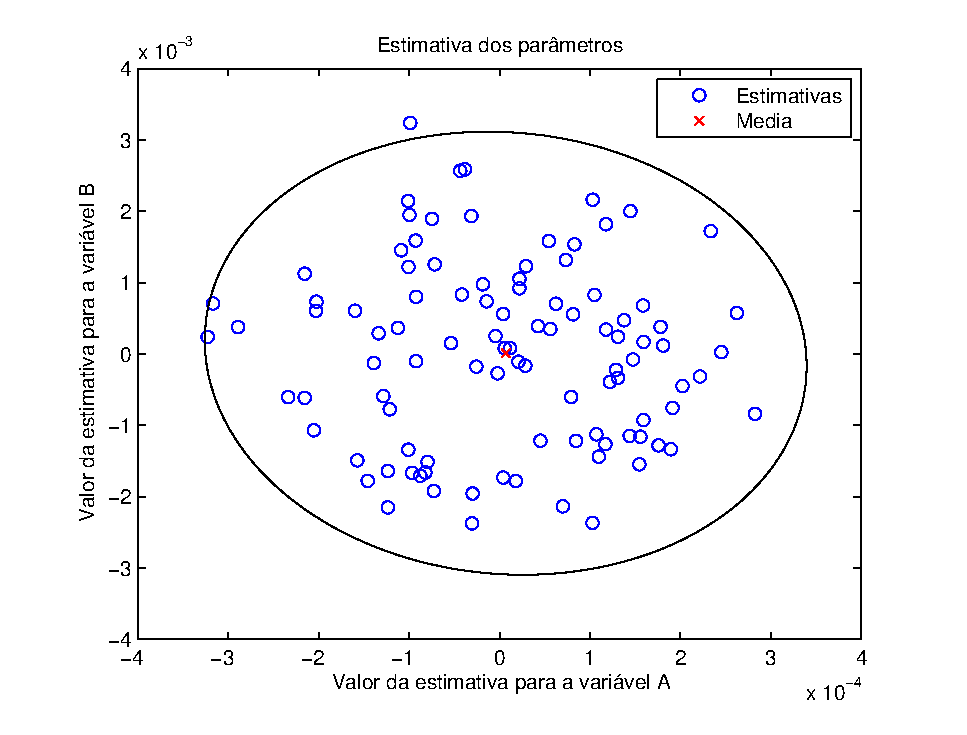
\includegraphics[width=0.8\columnwidth]{figures/si_covar_elipse.eps}
	\caption{Estimativas de um sistema e a regi�o de confian�a para $\chi$ de 95\%}
	\label{fig:si_covar_elipse}
\end{figure}



%===============================================================================
\section{Projeto de Experimento}
\label{sec:si_project_experiments}
%===============================================================================

Projeto de experimentos pode ser entendido como o procedimento para que se escolha o melhor 
sinal de entrada para a identifica��o dos par�metros desejados para o experimento. 
Desta forma muitas vari�veis podem ser levadas em considera��o, refletindo em propriedades que
podem ou n�o ser o foco do projeto de experimentos.

Uma forma de organizar o projeto de experimentos � desenvolve-lo como um problema de otimiza��o 
convexa, onde entre muitas vantagens est� o fato de que � poss�vel a utiliza��o de m�todos matem�ticos
para o c�lculo e sua formula��o pode ser feita por LMIs ({\it{Linear Matrix Inequality}}. Em \cite{jansson}
este t�pico � explorado em mais profundidade, sendo aqui apenas apresentado a sua ideia b�sica.

O projeto de experimento � uma alternativa ao uso de sinais como PRBS ({\it{Pseudo Randon Binary Sequence}}).
A escolha de um sinal mais apropriado para o experimento traz diversas vantagens, que podem ser bastante
significativas para o tempo e esfor�o despendido sobre o projeto do controlador, ou da identifica��o do sistema.
Uma destas vantagens � o tempo de dados coletados, aplicando-se sinais com componentes de frequ�ncia que s�o
mais informativos, tem-se uma efici�ncia maior nos dados amostrados, bastando um montante menor de data, para que
sejam obtidos os mesmos �ndices de qualidade, quando comparado com projetos utilizando sinais mais simples.

%===============================================================================
\subsection{Sinais de entrada mais comumente utilizados}
\label{sec:si_project_signal_input}
%===============================================================================

Como foi apresentado na Se��o \ref{sec:si_data_persistently_excitation} �
poss�vel formar sinais persistentes, apenas adicionando um n�mero suficiente de componentes
de frequ�ncia a fim de que todos os par�metros possam ser estimados. N�o � estranho
que se pense que quanto mais componentes tiver o sinal, melhor. 

Desta maneira, v�rios sinais que podem ser gerados de maneira f�cil e que possuem 
um grande range de componentes de frequ�ncia foram elaborados.

%===============================================================================
\subsubsection{Sinal Bin�rio Rand�mico}
\label{sec:si_project_signal_input_rbs}
%===============================================================================

Um sinal bin�rio por defini��o assume apenas dois valores (0 ou 1). Partindo deste
principio, um sinal bin�rio rand�mico, � uma sequencia aleat�ria de zeros e uns, que
formam o sinal.

A forma mais simples para a gerar este sinal �, baseado em um ru�do Gausiano branco
de m�dia zero, aplicar um filtro linear previamente escolhido. Assim pode-se teoricamente
gerar qualquer sinal bin�rio de qualquer n�vel.

O inconveniente desta forma � que aplicando um filtro ao sinal Gausiano ir� alterar o
seu espectro, n�o sendo a forma desta altera��o algo conhecido. Deve-se ent�o sempre 
antes de aplicar o sinal no sistema, deve-se verificar o espectro gerado. \cite{ljung}

%===============================================================================
\subsubsection{Sinal Bin�rio Pseudo-Rand�mico - PRBS}
\label{sec:si_project_signal_input_prbs}
%===============================================================================
% ref: ljung pages 418

Um {\it{sinal bin�rio pseudo-rand�mico}} � um sinal peri�dico com algumas propriedades
semelhantes a de ru�do branco. Este sinal � gerado pela equa��o:

\begin{equation}
u(t)=rem(A(z)u(t), 2)=rem(a_1 u(t-1)+...+a_n u(t-n), 2)
\label{eq:si_project_signal_prbs}
\end{equation}
onde $rem(x, 2)$ � o resto inteiro da divis�o de $x$ por 2. O sinal $u(t)$ deve ser peri�dico 
de pelo menos $2^n$ valores diferentes, como uma sequencia de zeros n�o � um sinal v�lido, por ser nulo, 
temos que o m�ximo per�odo � de tamanho $M=2^n -1$. Na verdade o per�odo vai depender da
escolha de $A(z)$. Pode-se entretanto mostrar que para cada $n$ existem escolhas de $A(z)$ que 
proporcionam o tamanho m�ximo. Tais escolhas s�o apresentadas na Tabela \ref{table:si_project_input_prbs}.
\cite{ljung}

\begin{table*}[htbp]
\begin{center}
\caption{Polin�mios $A(z)$ que geram o m�ximo per�odo $M$ para sinais PRBS de ordem $n$. $a_k=1$ para os $k$
   	indicados, 0 para os demais. Diversas outras escolhas existem para os mesmos $n$.}
\label{table:si_project_input_prbs}
\begin{tabular}{ccc}
\hline
        Ordem $n$ & $M=2^n-1$ & $a_k$ n�o zeros para $k$   \\
\hline
        2       & 3        & 1, 2       \\
        3       & 7        & 2, 3       \\
        4       & 15       & 1, 4       \\
        5       & 31       & 2, 5       \\
        6       & 63       & 1, 6       \\
        7       & 127      & 3, 7       \\
        8       & 255      & 1, 2, 7, 8 \\
        9       & 511      & 4, 9       \\
        10      & 1023     & 7, 10      \\
        11      & 2047     & 9, 11      \\
\hline
\end{tabular}
\end{center}
\end{table*}

O espectro de um sinal PRBS � dado por:

\begin{equation}
\Phi_u(\omega)=\frac{2 \pi \bar{u}^2}{M}\sum_{k=1}^{M-1}\delta (\omega -2 \pi k/M), \;\; 0\le \omega < 2 \pi
\label{eq:si_project_signal_prbs_spectrum}
\end{equation}

Observa-se que este � um sinal persistentemente excitante de ordem $M-1$. Na Figura 
\ref{fig:si_project_prbs} � apresentado um exemplo de sinal PRBS para $n=7$.

\begin{figure}[htbp]
	\center
	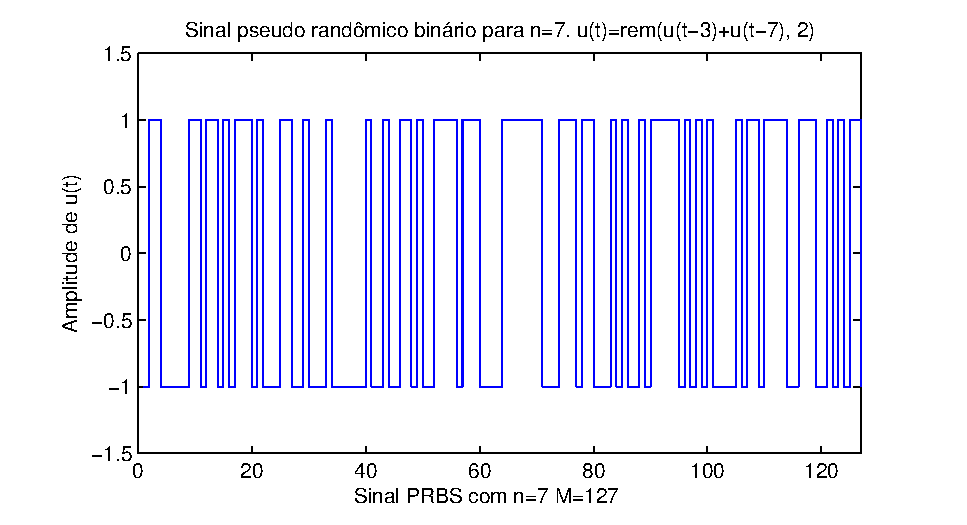
\includegraphics[width=0.95\columnwidth]{figures/si_project_prbs.eps}
	\caption{Sinal PRBS para $n=7$}
	\label{fig:si_project_prbs}
\end{figure}

As vantagens e desvantagens do sinal PRBS comparado com um sinal bin�rio rand�mico pode ser listado: \cite{ljung}

\begin{enumerate}[(I)]
\item Se o PRBS possuir per�odos inteiros a sua matriz de covari�ncia ter� alguns padr�es bem espec�ficos que permitem 
analiticamente se fa�a uma invers�o desta matriz. Isso facilita certas computa��es.
\item Existem essencialmente apenas um PRBS para cada escolha de $A(z)$. Diferentes valores iniciais apenas deslocam a
sequencia.
\item Para que as propriedades vantajosas do PRBS possam ser utilizadas, � necess�rio que um numero inteiro de per�odos
seja utilizado, o que limita a escolha do tamanho do experimento.
\end{enumerate}

%===============================================================================
\subsubsection{Ruido Branco Filtrado}
\label{sec:si_project_signal_input_wn_filtered}
%===============================================================================

Um das escolhas mais simples de sinais, � gerar um ru�do Gausiano e ent�o filtra-lo com 
algum filtro linear. Desta forma, teoricamente, � poss�vel de se atingir qualquer espectro de
sinal, bastando apenas a correta escolha do filtro. Como este sinal � gerado {\it{off-line}}, 
� poss�vel aplicar filtros n�o causais e eliminar efeitos transientes do sinal, o que
proporciona um comportamento espectral melhor. \cite{campestrini, ljung}

%===============================================================================
\subsection{Projeto de experimento visto como um problema de otimiza��o}
\label{sec:si_project_optimization}
%===============================================================================

O problema de projeto de experimento pode ser considerado como uma forma geral apresentada em:

\begin{equation}
\begin{matrix}
\underset{\Phi_{\chi_0}}{\text{minimize}} &  & \text{Objetivo}\\ 
\text{Sujeito a:} &  & \text{Requisitos de qualidade}\\ 
 &  & \text{Requisitos de sinais}
\end{matrix}
\label{eq:si_project_optimization}
\end{equation}

De forma geral os requisitos de qualidades s�o fun��es da covari�ncia de $P$. Por esta raz�o � natural usar
o espectro da entrada $\Phi_u$ e eventualmente o espectro cruzado $\Phi_{ue}$ como vari�veis do projeto.
A inclus�o de limita��es nos sinais e sua inclus�o como vari�veis de projeto s�o �teis para evitar que se chegue
em resultados onde a energia de entrada precise ser infinita para se obter os crit�rios desejados, ou largura
de banda que n�o s�o facilmente ating�veis em projetos reais.

T�picos projetos de experimentos s�o intrat�veis em sua forma original, pelos seguintes motivos: \cite{jansson}

\begin{enumerate}[I]
\item Algumas restri��es s�o tipicamente n�o convexas, e problemas com estas caracter�sticas podem ser dif�ceis
de resolver.
\item Existem restri��es que s�o de dimens�o infinita, o que exigem um certo grau de cuidado no procedimento de
otimiza��o.
\item Existe ainda o problema de encontrar um sinal realiz�vel que tenha as propriedades desejadas para o espectro.
\item A vari�ncia assint�tica depende tipicamente dos par�metros do sistema $\theta_0$, $P=P(\theta_0)$ que s�o
desconhecidos.
\end{enumerate}

Os primeiros 3 itens listados acima s�o contorn�veis pela inser��o de uma parametriza��o finita do espectro de entrada
e algumas vezes at� do espectro cruzado, tornando o problema convexo, que pode ser tratado de forma bem mais f�cil.

O �ltimo item onde a solu��o do problema depende das caracter�sticas do sistema a ser identificado � intr�nseco de quase
todos os problemas de otimiza��o, sendo ent�o inevit�vel. Em problemas reais este fato pode ser contornado utilizando alguns
m�todos conhecidos. \cite{jansson}

A formula��o de um projeto de experimento pode ser particionado nas seguintes partes:

\renewcommand{\labelitemi}{$\bullet$}
\begin{itemize}

\item {\it{Parametriza��o do espectro}}

A escolha de usar uma parametriza��o finita do espectro ou uma parametriza��o parcial da correla��o � regido pelos seguintes
aspectos:

\begin{itemize}
\item Relativos a otimiza��o
\item Computacionais
\item Limita��o de sinais
\item Robustez
\end{itemize}

A parametriza��o parcial da correla��o � �tima e pode usar um n�mero m�nimo de par�metros, utilizando assim, menos processamento
computacional. Entretanto certas limita��es de sinais n�o podem ser garantidas nesta situa��o, e a parametriza��o
pode depender do sistema real. Parametriza��o finita do espectro geralmente n�o atinge um m�nimo global mas as fun��es bases
n�o precisam ser fun��es do sistema real. Este m�todo pode gerenciar problemas de limita��es de sinal de frequ�ncia por frequ�ncia.
%-------------------------
\item {\it{Restri��es de qualidade}}

Assumindo que erros de vari�ncia s�o de grande import�ncia � natural que qualquer medida de qualidade do modelo leve em conta 
a matriz de covari�ncia $P$. Esta matriz pode ser manipulada pelos espectros de entrada $\Phi_{u}$ e o espectro cruzado $\Phi_{ue}$
como apresentado em \eqref{eq:si_project_optimization_quality}.

\begin{equation}
P^{-1}(\theta_0)=\frac{1}{2 \pi \lambda_0}\int_{-\pi}^{\pi}\mathcal{F}(e^{j\omega}, \theta_0)\begin{bmatrix}
\Phi_u(\omega) & \Phi_{ue}(\omega)\\ 
\Phi_{ue}^{0}(\omega) & \lambda_0 
\end{bmatrix}\mathcal{F}(e^{j\omega}, \theta_0)\;d\omega
\label{eq:si_project_optimization_quality}
\end{equation}

O principal desafio neste ponto � tornar as restri��es convexas em $P^{-1}$.

%-------------------------
\item {\it{Restri��es de sinal}}

Podem ser inclu�dos, restri��es de energia para os sinais de entrada e sa�da do sistema bem como restri��es no sinal dependentes da
frequ�ncia deste.
%-------------------------
\item {\it{Restri��es de robustez}}

A solu��o de boa parte dos problemas de otimiza��o recaem na necessidade de se conhecer o sistema real. Isso nem sempre � poss�vel 
e uma das formas de contornar este problema � substituir o sistema real por uma aproxima��o deste. Devido aos erros de estimativa deste
sistema, tem-se a necessidade de se utilizar m�todos que garantam robustez deste sistema, para que quando submetido ao sistema real, 
o projeto ainda seja v�lido.
%-------------------------
\end{itemize}



%===============================================================================
\section{Considera��es Finais}
\label{sec:si_conclusions}
%===============================================================================

Neste capitulo foram apresentados os principais aspectos de um projeto para identifica��o 
de sistemas. Partindo-se da escolha do sinal de excita��o para o experimento onde podemos 
determinar o que � de fundamental import�ncia para a identifica��o e focar os esfor�os para
reduzir ao m�ximo erros nestes aspectos.

Apresentou-se neste quesito de projeto de experimento, a ideia de tornar a escolha do sinal, um
problema de otimiza��o, onde as restri��es s�o as margens de qualidade que desejamos para as
propriedades assint�ticas da estimativa, limita��es de sinais que conseguimos produzir e margens de 
robustez.

Apresentou-se conceitos sobre a escolha do modelo que ser� utilizado para caracterizar o sistema
observado e as propriedades assint�ticas da estimativa para casos onde o sistema real $\mathcal{S}$ n�o
faz parte da fam�lia de modelos $\mathcal{M}$. Esta situa��o onde o sistema real n�o consegue ser
representado completamente pelo modelo adotado, faz com que erros de polariza��o e de vari�ncia 
recaiam sobre a estimativa atingida. Tamb�m foram apresentados os modelos mais comumente utilizados
para a identifica��o de sistemas lineares.

De posse dos dados coletados e da fam�lia de modelos que acredita-se conter o sistema real, � poss�vel, 
com a ajuda de preditores, determinar os par�metros do modelo que descrevem o comportamento do sistema
observado.

Elege-se ent�o uma fun��o dependente do erro entre os dados coletados e os dados gerados pelo preditor. 
Afim de que se tenha a melhor estimativa poss�vel, m�todos de minimiza��o s�o utilizados para que esta 
fun��o dependente do erro, seja minimizada. Obtendo-se assim a melhor estimativa poss�vel 
para aquele conjunto de dados, modelo e crit�rio de minimiza��o escolhidos.

� percept�vel que a identifica��o de um sistema � uma tarefa que depende de um grande conjunto
relativamente grande de de fatores. De um lado isso � extremamente interessante, pois temos liberdade
de escolha e a possibilidade de focar nosso projeto pontos que s�o mais interessantes, em detrimento
de outros que n�o s�o relevantes para o sistema em quest�o. Por outro lado temos um conjunto de
vari�veis que, se n�o compreendidas corretamente, podem tornar este processo algo oneroso e muitas
vezes at� ineficiente.



%===============================================================================



%===============================================================================
\chapter{Identifica��o de sistemas n�o lineares de tempo discreto}
\label{chapter:nlin_si_ident}
%===============================================================================
% idea: Colocar aqui neste capitulo todas as defini��es genericas sobre 
% n�o linearidades. coisas que na� sao relacionadas com o que eu vou fazer, ou que n�o
% sao conseguencia dela.
%
% lineariza��o: Descrever que muitas aplica�oes de identifica��o de sis nonlineares �
% linearizar ele em torno de um ponto. que isso ja eh bom suficiente.
%
% Models: Descrever os tipos de modelos para descrever sistemas nao lineares. Aqui 
% da para escrever bastante coisa. existem muito tipo de modelos para isso.
%
% Algoritmos: aqui vai o algoritmo do aguirre para modelos racionais. Talvez fosse de
% pensar em colcar isso no capitulo com minhas contribui��es? acho que nao .. referencio isso
% no meu capitulo.
%
% Conclus�es: Resumo do que foi visto aqui 

Anteriormente foram introduzidos conceitos b�sicos de identifica��o de sistemas lineares invariantes no tempo.
Este cap�tulo tem como objetivo apresentar os principais conceitos para identifica��o de sistemas n�o lineares de tempo
discreto.

Na Se��o \ref{sec:nlin_si_basic} ser�o apresentados conceitos b�sicos sobre n�o linearidades, algumas das principais
n�o linearidades encontradas e uma breve descri��o de suas caracter�sticas.

Na Se��o \ref{sec:nl_models} ser�o apresentados alguns modelos tipicamente utilizados para caracteriza��o de sistemas
n�o lineares. Na Se��o \ref{sec:nl_models_narmax} ser� dado �nfase aos modelos {\it{NARMAX}} e na Se��o
\ref{sec:nl_si_algorithms_rationals} ser� apresentado um algoritmo para a identifica��o de sistemas n�o lineares quando
descritos por esta estrutura de modelos. No Apendice \ref{appendix:rational_base_functions} s�o apresentadas as rotinas
desenvolvidas em Matlab para o desenvolvimento deste algoritmo.

Ao fim, ser�o apresentados breves conclus�es sobre identifica��o de sistemas n�o lineares (Se��o
\ref{sec:nl_conclusions}).

%===============================================================================
%===============================================================================
\section{Conceitos b�sicos}
\label{sec:nlin_si_basic}
%===============================================================================

Muitos, se n�o todos, os sistemas reais s�o n�o lineares. Existe entretanto um grande n�mero destes sistemas que
podem, e assim o s�o, representados por sistemas lineares em determinadas faixas de opera��o. Os sistemas desta
forma conseguem representar satisfatoriamente o sistema observado. Todavia alguns sistemas para serem
linearizados exigem uma faixa de atua��o muito estreita, fazendo com que o sistema em sua opera��o normal j� saia desta
faixa, tornando o modelo linear n�o representativo para aquele sistema em quest�o.

Tem-se desta forma uma das justificativas de escolher um modelo n�o linear para caracterizar o sistema. Ganha-se de um
lado no quesito de faixa de atua��o mais ampla e perde-se por abdicar da simplicidade de sistemas lineares.

Um sistema n�o linear pode ser genericamente descrito por:

\begin{equation}
y(t)=f(u(t), e(t))
\label{eq:nlin_system}
\end{equation}
onde $f(\cdot)$ � uma fun��o n�o linear dependente do sinal de entrada $u(t)$, e do ru�do do sistema $e(t)$. $y(t)$
� definido como a sa�da deste sistema.

%===============================================================================
\subsection{Tipos de n�o linearidades}
\label{sec:nlin_si_basic_types}
%===============================================================================
% Khalil
% ljng 		142
% Aguirre

Existem duas limita��es b�sicas para sistemas linearizados. Primeiro que a lineariza��o
� uma aproxima��o ao redor do ponto de opera��o, logo ele pode prever apenas o comportamento
nesta localidade do sistema e n�o o comportamento global. Segundo, as din�micas
de sistemas n�o lineares s�o muito mais ricas que as de sistemas lineares. Existem portanto alguns
fen�menos {\it{essenciais}}, n�o lineares, que n�o conseguem ser descritos ou
preditos por modelos lineares, estes s�o: \cite{khalil}

\renewcommand{\labelitemi}{$\bullet$}
\begin{itemize}

\item Tempo de fuga finito

O estado de um sistema linear inst�vel tende ao infinito na medida que o tempo 
tende ao infinito. Um sistema n�o linear est�vel, entretanto, pode ir para o
infinito em um tempo finito.


\item M�ltiplos pontos de equil�brios isolados

Um sistema linear assintoticamente est�vel tem apenas um ponto de equil�brio. Desta forma, este sistema pode
ter apenas um ponto do espa�o de estados que atraem o estado do sistema, independentemente
do estado inicial. Um sistema n�o linear pode ter mais de um ponto de equil�brio isolado. 
Desta forma o estado do sistema pode convergir para um destes equil�brios ou outro,
dependendo do estado inicial.

\item Ciclos limites

Para um sistema linear e invariante no tempo oscilar ele deve ter um par de autovalores
sobre o eixo imagin�rio, o que � uma condi��o n�o robusta praticamente imposs�vel de manter
na presen�a de perturba��es. Mesmo que isso seja poss�vel de manter, a amplitude da 
oscila��o depender� das condi��es iniciais do sistema. Na vida real, oscila��es est�veis
s�o atingidas apenas com sistemas n�o lineares. Alguns sistemas possuem oscila��es com
amplitude e frequ�ncia constantes, independente das condi��es iniciais. Chama-se isso de
ciclos limites.

\item Sub harm�nicas, harm�nicas ou oscila��es quase peri�dicas 

Um sistema linear est�vel sob uma entrada senoidal peri�dica produz uma sa�da senoidal na mesma frequ�ncia.
Sistemas n�o lineares alimentados por sinais peri�dicos podem oscilar com frequ�ncias que
podem ser sub m�ltiplos ou m�ltiplos da frequ�ncia de entrada.

\item Caos

Um sistema n�o linear pode ter um espa�o de estados mais complexo e seu comportamento n�o 
pode ser descrito por equil�brio, oscila��es peri�dicas ou quase peri�dicas. Este comportamento
normalmente � conhecido como caos. Alguns destes movimentos ca�ticos exibem comportamento
rand�mico, independentemente da natureza do sistema.

\item M�ltiplos modos de comportamento

N�o � incomum para dois ou mais modelos exibirem o comportamentos diferentes para um mesmo sistema n�o-linear.Um sistema
n�o for�ado pode ter mais de um ciclo limite. Um sistema for�ado com excita��o pode exibir harm�nicas, sub-harm�nicas, ou
comportamentos mais complicados, dependendo da frequ�ncia e amplitude da entrada. Ele pode exibir um pulo descontinuo no
modo de comportamento mesmo com mudan�as pequenas na amplitude e frequ�ncia de entrada do sinal.

\end{itemize}




%===============================================================================
\section{Modelos para sistemas n�o lineares}
\label{sec:nl_models}
%===============================================================================
% ideia aqui � colocar uma pequena introdu��o sobre modelos.. no mesmo estilo
% que foi para sistemas lineares.

Fam�lias ou conjuntos de modelos para sistemas podem ser divididos em dois grupos principais, baseados na natureza de
suas n�o linearidades: n�o linearidades est�ticas, onde a din�mica do sistema pode ser bem caracterizada por um modelo
linear enquanto que a parte n�o linear est� concentrada ou na entrada ou na sa�da do sistema de forma est�tica.
Para estes sistemas a forma mais usual de caracterizar � utilizando a classe de modelos de Wiener para n�o linearidades
na sa�da do processo ou a classe de Hammerstein, quando a n�o linearidade est� na entrada do processo.

Para os demais casos, onde a n�o linearidade est� na din�mica do processo existem v�rias fam�lias de modelos
que podem ser utilizados como ser� visto no decorrer deste cap�tulo. De forma geral todos estes conjuntos
possuem em comum a ideia da escolha de uma base que seja representativa e que possa reduzir a quantidade de
termos a ser identificado e com isso ter uma boa aproxima��o do sistema real com a menor quantidade de
par�metros poss�vel na identifica��o.

Percebe-se ent�o que um mesmo sistema pode ser representado por diversos destes modelos, mas dependendo das
caracter�sticas deste sistema, uma das fam�lias ser� mais adequada, por sua base possuir mais
afinidade em representar certos tipos de n�o linearidades.

Um dos passos mais desafiadores na constru��o de modelos n�o lineares � a escolha da estrutura de
modelo. Quando este modelo � n�o linear, existe uma grande quantidade de op��es e com isso o perigo
de escolher um modelo desnecessariamente complexo � evidente. Isso baseia-se no {\it{principio
da parcim�nia}} que basicamente determina que o modelo deve ser o mais simples poss�vel.
\cite{aguirre_maps}

%TODO: achar onde por isso e se nao tem nada melhor no paper para adicionar
%Um problema fundamental referente a modelos parametrizados refere-se ao fato do
%par�metro poder ou n�o ser determinado a partir dos valores medidos de entrada e sa�da. \cite{glad_ljung}

% ===============================================================================
\subsection{Modelos de Wiener e Hammerstein}
\label{sec:nl_models_wiener_hammerstein}
% Aguirre: 334
% ljung 143
%===============================================================================

Modelos de Wiener e Hammerstein s�o normalmente utilizados em situa��es onde a din�mica do sistema pode ser bem
descrita por um sistema linear, mas existem algumas n�o linearidades est�ticas atreladas a entrada
e/ou a sa�da. Este ser� o caso de atuadores n�o lineares com caracter�sticas como satura��o, zona morta, entre outros.

Um modelo com n�o linearidades na entrada � chamado de {\it{modelo de Hammerstein}} e 
para n�o linearidades na sa�da chama-se {\it{modelo de Wiener}}. \cite{ljung}

Na Figura (\ref{fig:nl_models_hammerstein_wiener}) observa-se o diagrama de bloco para os modelos
de Hammerstein e Wiener.


\begin{figure}[htbp]
\center
\scalebox{1} % Change this value to rescale the drawing.
{
\begin{pspicture}(0,-1.6)(9.439062,1.6)
\usefont{T1}{ptm}{m}{n}
\rput(0.52453125,1.31){$u(t)$}
\usefont{T1}{ptm}{m}{n}
\rput(3.9557812,1.31){$f(u(t))$}
\usefont{T1}{ptm}{m}{n}
\rput(7.554531,1.35){$y(t)$}
\usefont{T1}{ptm}{m}{n}
\rput(5.8759375,1.15){Modelo}
\usefont{T1}{ptm}{m}{n}
\rput(5.7834377,0.75){Linear}
\usefont{T1}{ptm}{m}{n}
\rput(2.1957812,1.03){$f(\cdot)$}
\psframe[linewidth=0.04,dimen=outer](3.0,1.6)(1.2,0.4)
\psframe[linewidth=0.04,dimen=outer](6.8,1.6)(5.0,0.4)
\psline[linewidth=0.04cm,arrowsize=0.05291667cm 2.0,arrowlength=1.4,arrowinset=0.4]{->}(3.0,1.0)(5.0,1.0)
\psline[linewidth=0.04cm,arrowsize=0.05291667cm 2.0,arrowlength=1.4,arrowinset=0.4]{->}(0.0,1.0)(1.2,1.0)
\psline[linewidth=0.04cm,arrowsize=0.05291667cm 2.0,arrowlength=1.4,arrowinset=0.4]{->}(6.8,1.0)(8.0,1.0)
\usefont{T1}{ptm}{m}{n}
\rput(0.52453125,-0.69){$u(t)$}
\usefont{T1}{ptm}{m}{n}
\rput(3.9357812,-0.69){$z(t)$}
\usefont{T1}{ptm}{m}{n}
\rput(2.0759375,-0.85){Modelo}
\usefont{T1}{ptm}{m}{n}
\rput(1.9834375,-1.25){Linear}
\usefont{T1}{ptm}{m}{n}
\rput(5.9957814,-0.99){$f(\cdot)$}
\psframe[linewidth=0.04,dimen=outer](3.0,-0.4)(1.2,-1.6)
\psframe[linewidth=0.04,dimen=outer](6.8,-0.4)(5.0,-1.6)
\psline[linewidth=0.04cm,arrowsize=0.05291667cm 2.0,arrowlength=1.4,arrowinset=0.4]{->}(3.0,-1.0)(5.0,-1.0)
\psline[linewidth=0.04cm,arrowsize=0.05291667cm 2.0,arrowlength=1.4,arrowinset=0.4]{->}(0.0,-1.0)(1.2,-1.0)
\psline[linewidth=0.04cm,arrowsize=0.05291667cm 2.0,arrowlength=1.4,arrowinset=0.4]{->}(6.8,-1.0)(8.0,-1.0)
\usefont{T1}{ptm}{m}{n}
\rput(8.204532,-0.65){$y(t)=f(z(t))$}
\end{pspicture} 
}
\caption{Acima: modelo de Hammerstein. Abaixo: Modelo de Wiener.}
\label{fig:nl_models_hammerstein_wiener}
\end{figure}

%===============================================================================
\subsection{Serie de volterra}
\label{sec:nl_models_volterra}
% Aguirre 334
%===============================================================================

Um sistema n�o linear pode ser descrito pela serie de Volterra \eqref{eq:nl_models_volterra}:

\begin{equation}
y(t)=\sum_{j=1}^{\infty}\int_{-\infty}^{\infty}\cdots \int_{-\infty}^{\infty}
h_j(\tau_1, ... ,\tau_j) \prod_{i=1}^{j}u(t-\tau_i)d\tau_i
\label{eq:nl_models_volterra}
\end{equation}

Onde $h_j$ s�o generaliza��es n�o lineares da resposta ao impulso $h_1(t)$ . Para
um sistema linear com $j=1$ a equa��o de Volterra se reduz a integral de convolu��o.
\cite{aguirre}

As expans�es funcionais em series de Volterra relacionam os sinais passados da entrada com o valor atual da sa�da do
sistema e isso inevitavelmente significa que que um conjunto excessivo de par�metros � necess�rio para descrever at� mesmo
simples sistemas n�o lineares e consequentemente apenas poucas aplica��es pr�ticas foram apresentadas.
\cite{chen_billings1989}

%===============================================================================
\subsection{Redes Neurais}
\label{sec:nl_models_neurals}
% TODO: Search for bib
%===============================================================================
As redes neurais artificiais s�o compostas por camadas de neur�nios interconectados. A sa�da de um
neur�nio com $n$ entradas � apresentado na equa��o \eqref{eq:nl_models_neural}

\begin{equation}
x=\emph{f}\left ( \sum_{j=1}^{n}\omega_j x_j +b \right )
\label{eq:nl_models_neural}
\end{equation}

Sendo $b$ (bias) e $\omega_j$ constantes. $\emph{f}(\cdot)$ � chamada fun��o de ativa��o. A
fun��o de ativa��o mais comum �: \cite{aguirre}

\begin{equation}
\emph{f}(z)=\frac{1}{1+e^{-z}}
\nonumber
\end{equation}


%===============================================================================
\subsubsection{Redes Neurais multi-camadas}
\label{sec:nl_models_neurals_multilayer}
%===============================================================================

Uma tipica rede multi-camadas pode ser descrita como na Figura
(\ref{fig:nl_models_neural_multilayer}).  Na pratica redes neurais multi-camadas tem grande apelo no
reconhecimento de padr�es. Do ponto de vista te�rico os sistemas de redes multi-camadas podem ser
considerados como mapas n�o lineares onde os elementos das matrizes de peso s�o os par�metros.
\cite{narenda_parthasarathy}

\begin{figure}[htbp]
\center
\scalebox{0.85} % Change this value to rescale the drawing.
{
\begin{pspicture}(0,-3.369375)(14.589063,3.329375)
\pscircle[linewidth=0.04,dimen=outer](4.77,2.729375){0.4}
\usefont{T1}{ptm}{m}{n}
\rput(4.804531,2.699375){$\sum$}
\psframe[linewidth=0.04,dimen=outer](7.17,3.329375)(5.97,2.129375)
\usefont{T1}{ptm}{m}{n}
\rput(6.534531,2.759375){$\gamma$}
\pscircle[linewidth=0.04,dimen=outer](4.77,0.529375){0.4}
\usefont{T1}{ptm}{m}{n}
\rput(4.804531,0.499375){$\sum$}
\psframe[linewidth=0.04,dimen=outer](7.17,1.129375)(5.97,-0.070625)
\usefont{T1}{ptm}{m}{n}
\rput(6.534531,0.559375){$\gamma$}
\pscircle[linewidth=0.04,dimen=outer](4.77,-1.870625){0.4}
\usefont{T1}{ptm}{m}{n}
\rput(4.804531,-1.900625){$\sum$}
\psframe[linewidth=0.04,dimen=outer](7.17,-1.270625)(5.97,-2.470625)
\usefont{T1}{ptm}{m}{n}
\rput(6.534531,-1.840625){$\gamma$}
\pscircle[linewidth=0.04,dimen=outer](10.37,2.729375){0.4}
\usefont{T1}{ptm}{m}{n}
\rput(10.384531,2.679375){$\sum$}
\psframe[linewidth=0.04,dimen=outer](12.77,3.329375)(11.57,2.129375)
\usefont{T1}{ptm}{m}{n}
\rput(12.254531,2.739375){$\gamma$}
\pscircle[linewidth=0.04,dimen=outer](10.37,0.529375){0.4}
\usefont{T1}{ptm}{m}{n}
\rput(10.384531,0.479375){$\sum$}
\psframe[linewidth=0.04,dimen=outer](12.77,1.129375)(11.57,-0.070625)
\usefont{T1}{ptm}{m}{n}
\rput(12.254531,0.539375){$\gamma$}
\pscircle[linewidth=0.04,dimen=outer](10.37,-1.870625){0.4}
\usefont{T1}{ptm}{m}{n}
\rput(10.384531,-1.920625){$\sum$}
\psframe[linewidth=0.04,dimen=outer](12.77,-1.270625)(11.57,-2.470625)
\usefont{T1}{ptm}{m}{n}
\rput(12.254531,-1.860625){$\gamma$}
\psline[linewidth=0.04cm,arrowsize=0.05291667cm 2.0,arrowlength=1.4,arrowinset=0.4]{->}(5.17,2.729375)(5.97,2.729375)
\psline[linewidth=0.04cm,arrowsize=0.05291667cm 2.0,arrowlength=1.4,arrowinset=0.4]{->}(5.17,0.529375)(5.97,0.529375)
\psline[linewidth=0.04cm,arrowsize=0.05291667cm 2.0,arrowlength=1.4,arrowinset=0.4]{->}(5.37,-1.870625)(5.97,-1.870625)
\psline[linewidth=0.04cm,arrowsize=0.05291667cm 2.0,arrowlength=1.4,arrowinset=0.4]{->}(10.77,2.729375)(11.57,2.729375)
\psline[linewidth=0.04cm,arrowsize=0.05291667cm 2.0,arrowlength=1.4,arrowinset=0.4]{->}(10.77,0.529375)(11.57,0.529375)
\psline[linewidth=0.04cm,arrowsize=0.05291667cm 2.0,arrowlength=1.4,arrowinset=0.4]{->}(10.77,-1.870625)(11.57,-1.870625)
\psline[linewidth=0.04cm,arrowsize=0.05291667cm 2.0,arrowlength=1.4,arrowinset=0.4]{->}(12.77,2.729375)(13.97,2.729375)
\psline[linewidth=0.04cm,arrowsize=0.05291667cm 2.0,arrowlength=1.4,arrowinset=0.4]{->}(12.77,0.529375)(13.97,0.529375)
\psline[linewidth=0.04cm,arrowsize=0.05291667cm 2.0,arrowlength=1.4,arrowinset=0.4]{->}(12.77,-1.870625)(13.97,-1.870625)
\usefont{T1}{ptm}{m}{n}
\rput(13.674531,3.039375){$y_1$}
\usefont{T1}{ptm}{m}{n}
\rput(13.674531,0.839375){$y_2$}
\usefont{T1}{ptm}{m}{n}
\rput(13.674531,-1.560625){$y_n$}
\psdots[dotsize=0.12](6.77,-0.470625)
\psdots[dotsize=0.12](6.77,-0.670625)
\psdots[dotsize=0.12](6.77,-0.870625)
\psdots[dotsize=0.12](12.37,-0.470625)
\psdots[dotsize=0.12](12.37,-0.670625)
\psdots[dotsize=0.12](12.37,-0.870625)
\psline[linewidth=0.04cm,arrowsize=0.05291667cm 2.0,arrowlength=1.4,arrowinset=0.4]{->}(7.1873198,2.729375)(9.97,2.729375)
\psline[linewidth=0.04cm,arrowsize=0.05291667cm 2.0,arrowlength=1.4,arrowinset=0.4]{->}(7.1873198,2.729375)(9.97,0.529375)
\psline[linewidth=0.04cm,arrowsize=0.05291667cm 2.0,arrowlength=1.4,arrowinset=0.4]{->}(7.1873198,2.729375)(9.97,-1.870625)
\psline[linewidth=0.04cm,arrowsize=0.05291667cm 2.0,arrowlength=1.4,arrowinset=0.4]{->}(7.1873198,0.529375)(9.97,0.529375)
\psline[linewidth=0.04cm,arrowsize=0.05291667cm 2.0,arrowlength=1.4,arrowinset=0.4]{->}(7.1873198,-1.870625)(9.97,-1.870625)
\psline[linewidth=0.04cm,arrowsize=0.05291667cm 2.0,arrowlength=1.4,arrowinset=0.4]{->}(7.1873198,0.529375)(9.97,2.729375)
\psline[linewidth=0.04cm,arrowsize=0.05291667cm 2.0,arrowlength=1.4,arrowinset=0.4]{->}(7.1873198,0.529375)(9.97,-1.870625)
\psline[linewidth=0.04cm,arrowsize=0.05291667cm 2.0,arrowlength=1.4,arrowinset=0.4]{->}(7.1873198,-1.870625)(9.97,0.529375)
\psline[linewidth=0.04cm,arrowsize=0.05291667cm 2.0,arrowlength=1.4,arrowinset=0.4]{->}(7.1873198,-1.870625)(9.97,2.729375)
\psline[linewidth=0.04cm,arrowsize=0.05291667cm 2.0,arrowlength=1.4,arrowinset=0.4]{->}(1.7888126,2.7075653)(4.37,2.7075653)
\psline[linewidth=0.04cm,arrowsize=0.05291667cm 2.0,arrowlength=1.4,arrowinset=0.4]{->}(1.7888126,2.7075653)(4.37,0.51799595)
\psline[linewidth=0.04cm,arrowsize=0.05291667cm 2.0,arrowlength=1.4,arrowinset=0.4]{->}(1.7888126,2.7075653)(4.37,-1.870625)
\psline[linewidth=0.04cm,arrowsize=0.05291667cm 2.0,arrowlength=1.4,arrowinset=0.4]{->}(1.7871279,0.529375)(4.37,0.529375)
\psline[linewidth=0.04cm,arrowsize=0.05291667cm 2.0,arrowlength=1.4,arrowinset=0.4]{->}(1.7871279,-1.850625)(4.37,-1.850625)
\psline[linewidth=0.04cm,arrowsize=0.05291667cm 2.0,arrowlength=1.4,arrowinset=0.4]{->}(1.7871279,0.529375)(4.37,2.729375)
\psline[linewidth=0.04cm,arrowsize=0.05291667cm 2.0,arrowlength=1.4,arrowinset=0.4]{->}(1.7871279,0.529375)(4.37,-1.870625)
\psline[linewidth=0.04cm,arrowsize=0.05291667cm 2.0,arrowlength=1.4,arrowinset=0.4]{->}(1.7871279,-1.850625)(4.37,0.5389402)
\psline[linewidth=0.04cm,arrowsize=0.05291667cm 2.0,arrowlength=1.4,arrowinset=0.4]{->}(1.7871279,-1.850625)(4.37,2.729375)
\usefont{T1}{ptm}{m}{n}
\rput(1.4745313,3.039375){$u_1$}
\usefont{T1}{ptm}{m}{n}
\rput(1.4745313,0.839375){$u_2$}
\usefont{T1}{ptm}{m}{n}
\rput(1.4745313,-1.560625){$u_n$}
\usefont{T1}{ptm}{m}{n}
\rput(1.4845313,-3.160625){$\text{Entrada}$}
\usefont{T1}{ptm}{m}{n}
\rput(6.7345314,-3.160625){$\text{Camada Oculta}$}
\usefont{T1}{ptm}{m}{n}
\rput(12.444531,-3.160625){$\text{Camada Sa�da}$}
\end{pspicture} 
}

\caption{Rede neural multi-camadas.}
\label{fig:nl_models_neural_multilayer}
\end{figure}

A sa�da do sistema para uma rede multi-camadas pode ser descrito como em
\eqref{eq:nl_models_neural_multilayer}.

\begin{equation}
y(t)=f_s\left \{ \sum_{i=1}^{m} \omega_i f_i \left ( \sum_{j=1}^{n}\omega_{ij} x_j + b_i \right ) +
b_s \right \}
\label{eq:nl_models_neural_multilayer}
\end{equation}

Sendo que $f_s$ � a fun��o de ativa��o do neur�nio da camada de sa�da. Esta fun��o n�o precisa ser
igual a $f_i$, $i=1, \ldots , m$ que por sua vez n�o precisam ser iguais entre si. $b_s$ � o termo
de polariza��o do neur�nio da camada de sa�da, $\omega_i$ s�o os pesos da sa�da de cada neur�nio da
camada oculta e $\omega_{ij}$ s�o os pesos da entrada $j$, vista pelo $i-$�simo neur�nio da camada
oculta. \cite{aguirre}

%===============================================================================
\subsubsection{Redes Neurais recorrentes}
\label{sec:nl_models_neurals_multilayer}
%===============================================================================

Redes neurais recorrentes, trabalho introduzido por Hopfield em \cite{hopfield} prov� uma
alternativa para o reconhecimento de padr�es. O m�todo proposto consiste em ter uma rede neural de
apenas uma camada adicionada de uma realimenta��o com um atraso de tempo como apresentado na Figura
(\ref{fig:nl_models_neural_recurrent}). \cite{narenda_parthasarathy}

\begin{figure}[htbp]
\center
\scalebox{0.85} % Change this value to rescale the drawing.
{
\begin{pspicture}(0,-5.4)(11.04,5.4)
\usefont{T1}{ptm}{m}{n}
\rput(8.015624,4.91){$\gamma$}
\usefont{T1}{ptm}{m}{n}
\rput(8.015624,3.31){$\gamma$}
\usefont{T1}{ptm}{m}{n}
\rput(8.215624,0.71){$\gamma$}
\usefont{T1}{ptm}{m}{n}
\rput(5.073437,-0.89){$z^{-1}$}
\pscircle[linewidth=0.04,dimen=outer](6.42,4.8){0.4}
\pscircle[linewidth=0.04,dimen=outer](6.42,0.6){0.4}
\pscircle[linewidth=0.04,dimen=outer](6.42,3.2){0.4}
\usefont{T1}{ptm}{m}{n}
\rput(6.395625,0.61){$\sum$}
\usefont{T1}{ptm}{m}{n}
\rput(6.395625,3.21){$\sum$}
\usefont{T1}{ptm}{m}{n}
\rput(6.395625,4.81){$\sum$}
\psdots[dotsize=0.12](5.82,4.8)
\psdots[dotsize=0.12](5.82,3.2)
\psdots[dotsize=0.12](5.82,0.6)
\psdots[dotsize=0.12](2.82,4.8)
\psdots[dotsize=0.12](2.82,3.2)
\psdots[dotsize=0.12](2.82,0.6)
\psline[linewidth=0.04cm](2.82,4.8)(5.82,4.8)
\psline[linewidth=0.04cm](2.82,4.8)(5.82,3.1916058)
\psline[linewidth=0.04cm](2.82,4.8)(5.82,0.61817497)
\psline[linewidth=0.04cm](2.82,0.61817497)(5.82,4.8)
\psline[linewidth=0.04cm](2.82,3.1916058)(5.82,4.8)
\psline[linewidth=0.04cm](2.82,3.1916058)(5.82,3.1916058)
\psline[linewidth=0.04cm](2.82,3.1916058)(5.82,0.61817497)
\psline[linewidth=0.04cm](2.82,0.61817497)(5.82,3.1916058)
\psline[linewidth=0.04cm](2.82,0.61817497)(5.82,0.61817497)
\psline[linewidth=0.04cm](8.8,0.6)(9.42,0.6)
\psline[linewidth=0.04cm](9.4,-1.0)(5.8,-1.0)
\psline[linewidth=0.04cm](4.62,-1.0)(1.6,-1.0)
\psline[linewidth=0.04cm](1.62,0.6)(2.82,0.6)
\psline[linewidth=0.04cm](6.82,0.6)(7.62,0.6)
\psline[linewidth=0.04cm](5.82,0.6)(6.0,0.6)
\psline[linewidth=0.04cm](6.82,3.2)(7.62,3.2)
\psline[linewidth=0.04cm](5.82,3.2)(6.02,3.2)
\psline[linewidth=0.04cm](5.82,4.8)(6.02,4.8)
\psline[linewidth=0.04cm](6.82,4.8)(7.62,4.8)
\psline[linewidth=0.04cm](8.8,3.2)(10.22,3.2)
\psline[linewidth=0.04cm](5.8,-2.6)(10.2,-2.6)
\psline[linewidth=0.04cm](8.8,4.8)(11.02,4.8)
\psline[linewidth=0.04cm](11.0,-4.8)(5.8,-4.8)
\psline[linewidth=0.04cm](4.62,-2.6)(0.8,-2.6)
\psline[linewidth=0.04cm](0.8,3.2)(2.82,3.2)
\psline[linewidth=0.04cm](2.82,4.8)(0.0,4.8)
\psline[linewidth=0.04cm](0.0,-4.8)(4.62,-4.8)
\psdots[dotsize=0.12](8.22,2.2)
\psdots[dotsize=0.12](8.22,2.0)
\psdots[dotsize=0.12](8.22,1.8)
\psdots[dotsize=0.12](5.22,-3.4)
\psdots[dotsize=0.12](5.22,-3.6)
\psdots[dotsize=0.12](5.22,-3.8)
\usefont{T1}{ptm}{m}{n}
\rput(9.864062,5.11){$x_1(t+1)$}
\usefont{T1}{ptm}{m}{n}
\rput(9.864062,3.51){$x_2(t+1)$}
\usefont{T1}{ptm}{m}{n}
\rput(9.864062,0.91){$x_n(t+1)$}
\usefont{T1}{ptm}{m}{n}
\rput(2.0040624,5.11){$x_1(t)$}
\usefont{T1}{ptm}{m}{n}
\rput(2.0040624,3.51){$x_2(t)$}
\usefont{T1}{ptm}{m}{n}
\rput(2.0040624,0.91){$x_n(t)$}
\usefont{T1}{ptm}{m}{n}
\rput(4.3840623,5.11){$\omega_i$}
\usefont{T1}{ptm}{m}{n}
\rput(5.073437,-2.49){$z^{-1}$}
\usefont{T1}{ptm}{m}{n}
\rput(5.073437,-4.69){$z^{-1}$}
\psframe[linewidth=0.04,dimen=outer](8.8,5.4)(7.6,4.2)
\psframe[linewidth=0.04,dimen=outer](8.8,3.8)(7.6,2.6)
\psframe[linewidth=0.04,dimen=outer](8.8,1.2)(7.6,0.0)
\psframe[linewidth=0.04,dimen=outer](5.8,-0.4)(4.6,-1.6)
\psframe[linewidth=0.04,dimen=outer](5.8,-2.0)(4.6,-3.2)
\psframe[linewidth=0.04,dimen=outer](5.8,-4.2)(4.6,-5.4)
\psline[linewidth=0.04cm](11.0,4.8)(11.0,-4.8)
\psline[linewidth=0.04cm](10.2,3.2)(10.2,-2.6)
\psline[linewidth=0.04cm](9.4,0.6)(9.4,-1.0)
\psline[linewidth=0.04cm](1.6,0.6)(1.6,-1.0)
\psline[linewidth=0.04cm](0.8,-2.6)(0.8,3.2)
\psline[linewidth=0.04cm](0.0,4.8)(0.0,-4.8)
\end{pspicture} 
}
\caption{Rede neural recorrentes.}
\label{fig:nl_models_neural_recurrent}
\end{figure}

%===============================================================================
\subsection{Fun��es Radiais de Base}
\label{sec:nl_models_radiais}
% Aguirre 337
%===============================================================================

Fun��es radiais de base  ({\it{RBF - Radial basis functions}})  s�o uma tradicional t�cnica para
interpola��o em espa�os multidimensional \cite{chen_billings_narmax} e podem ser descritos como
mapeamentos do tipo:

\begin{equation}
f(y)=w_0+\sum_{i}w_i \phi (\left \| y-c_i \right \|)
\label{eq:nl_models_rbf}
\end{equation}

Sendo que $y \in \mathbb{R}^{d_e}$ ($d_e$ � conhecido como dimens�o de imers�o),
$\left \| \cdot \right \|$ � a norma euclidiana, $w_i \in \mathbb{R}$ s�o pesos, 
$c_i \in \mathbb{R}^{d_e}$ s�o centros e $\phi(\cdot):\mathbb{R}^+ \to \mathbb{R}$ 
� uma fun��o, normalmente escolhida a priori, como por exemplo: \cite{aguirre}

\begin{equation}
\phi(\left \| y-c_i \right \|)= exp\left ( -\frac{\left \| y-c_i \right \|^2}{\sigma_i^2} \right )
\nonumber
\end{equation}

Outras fun��es de base usadas s�o apresentadas na Tabela \ref{table:nl_models_rbf}

\begin{table*}[htbp]
\begin{center}
\caption{Algumas fun��es Radiais de base comumente utilizadas.}
\label{table:nl_models_rbf}
\begin{tabular}{ll}
\hline
        Nome & Fun��o   \\
\hline
        Multi quadr�tica inversa  & $\phi(r)=(r^2+\sigma ^2)^{-1/2}$ \\ 
        Linear                    & $\phi(r)=r$                      \\ 
        C�bica                    & $\phi(r)=r^3$                    \\ 
        Multi-quadr�tica           & $\phi(r)=\sqrt{r^2+\sigma^2}$    \\ 
        {\it{Thin - plate spline}} & $\phi(r)=r^2\; \text{log}(r)$   \\ 
\hline
\end{tabular}
\end{center}
\end{table*}

Sendo que $r=\left \| y-c_i \right \|$ e $\sigma$ definem a largura do chap�u no caso de
fun��es Gausianas e das multi-quadr�ticas, como pode ser visto na figura (\ref{fig:nl_models_rbf}).

\begin{figure}[htbp]
	\center
	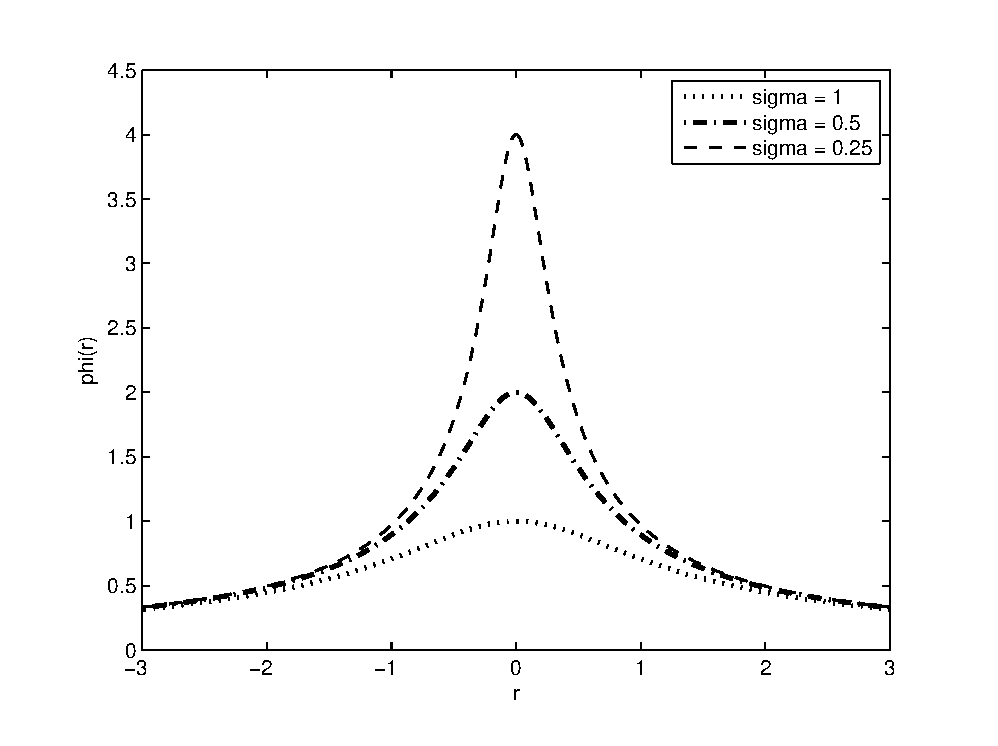
\includegraphics[width=0.8\columnwidth]{figures/nl_models_rbf.eps}
	\caption{Fun��o multiquadr�ticas inversa para alguns valores de $\sigma$.}
	\label{fig:nl_models_rbf}
\end{figure}

Este tipo de representa��o tem boas propriedades locais e pode ser interpretada como 
uma t�cnica de interpola��o global. Fun��es radiais de base s�o casos particulares
de redes neurais, porem neste caso lineares nos par�metros $w_i$.\cite{aguirre} 

No contexto de identifica��o de sistemas � comum adicionar termos auto-regressivos
lineares, bem como termos de entrada � equa��o \eqref{eq:nl_models_rbf} resultando em:

\begin{equation}
y(k)=w_0 + \sum_{i}w_i \phi(\left \| \mathbf{y}(k-1)-c_i \right \|)+\sum_{i=1}^{n_y}a_i y(k-i)+\sum_{i=1}^{n_u}b_i u(k-i)+e(k)
\nonumber
\end{equation}

Sendo $\mathbf{y}(k-1)=\begin{bmatrix}
y(k-1) & ... & y(k-n_y) & u(k-1) & ... & u(k-n_u)
\end{bmatrix}$.

%===============================================================================
\section{Modelos NARMAX}
\label{sec:nl_models_narmax}
% Aguirre 343
%===============================================================================

Os modelos {\it{NARX}} (do termo ingl�s {\it{nonlinear autoregressive model with exogenous variables}}) s�o modelos
discretos no tempo que caracterizam o valor da sa�da em fun��o dos valores passados da entrada e da pr�pria sa�da.
Algumas vezes, para evitar a polariza��o da estimativa dos par�metros adiciona-se termos do modelo do ru�do ao modelo
do sistema. Quando isso � feito o modelo passa a ser chamado de modelo {\it{NARMAX}} (do termo ingl�s {\it{nonlinear
autoregressive moving average model with exogenous variables}}), introduzido por \cite{leontaritis_billings1985}.

Este modelo prov� uma representa��o unificada para a descri��o de sistemas discretos n�o lineares:

\begin{equation}
y(t)=\theta^T\Phi_{nl}(y, u, e)
\label{eq:nlin_models_narmax_generic}
\end{equation}
onde $\Phi_{nl}(\cdot)$ denota um campo vetorial que depende dos valores passados de $y(t)$ e presente e passados de
$u(t)$ e $e(t)$; $\theta$ � o vetor de par�metros a ser identificado.

As classes de modelos NARMAX podem ent�o ser compreendidas como um conjunto ou somat�rio de fun��es n�o lineares, que
s�o parametrizados linearmente. Vale aqui esclarecer que a forma apresentada em \eqref{eq:nlin_models_narmax_generic}
n�o � uma regress�o linear. Para uma regress�o linear:

\begin{equation}
y(t)=\theta^T\phi(y(t), u(t))
\label{eq:nlin_models_narmax_reg}
\end{equation}
onde $\phi(\cdot)$ � dependente apenas dos sinais de entrada e sa�da do sistema, usualmente sendo uma matriz formada a
partir dos dados coletados do sistema. Diferentemente do equacionamento apresentado em
\eqref{eq:nlin_models_narmax_generic}, onde $\Phi_{nl}(\cdot)$ � dependente tamb�m do ru�do. Outra diferen�a est� no
fato de que em \eqref{eq:nlin_models_narmax_generic} � poss�vel ter regressores n�o lineares. 

Quando o vetor $\Phi_{nl}(\cdot)$ � um conjunto de fun��es polinomiais, o modelo pode ser apresentado como em :

\begin{equation}
y(t)=\sum_{i}c_i \prod_{j=1}^{n_y}y(t-j) \prod_{r=1}^{n_u}u(t-r) \prod_{q=0}^{n_e}e(t-q)
\label{eq:nl_model_narmax_pol}
\end{equation}

Os modelos polinomiais {\it{bilineares}} s�o casos particulares do modelo polinomial 
\eqref{eq:nl_model_narmax_pol} quando todos os termos n�o lineares s�o do tipo 
$y(t-i)u(t-j), \; \forall i,j$. \cite{aguirre}

Modelos racionais s�o formados pela raz�o entre dois polin�mios:

\begin{equation}
y(t)=\frac{\sum_{i}c_i \prod_{j=1}^{n_y}y(t-j) \prod_{r=1}^{n_u}u(t-r) \prod_{q=0}^{n_e}e(t-q)}
{\sum_{i}d_i \prod_{j=1}^{d_y}y(t-j) \prod_{r=1}^{d_u}u(t-r) \prod_{q=0}^{d_e}e(t-q)} + e(t)
\label{eq:nl_model_narmax_rat}
\end{equation}

Em fun��o de terem uma estrutura mais flex�vel, os modelos racionais podem vir a ser
mais abrangentes na modelagem de certos sistemas quando comparados com modelos polinomiais.
Entretanto, os modelos racionais s�o mais sens�veis ao ru�do. \cite{aguirre}

%===============================================================================
%===============================================================================
\subsection{Modelo polinomial}
\label{sec:nl_models_narmax_pol}
% Aguirre 343
%===============================================================================

Com rela��o ao modelo gen�rico polinomial {\it{NARMAX}} apresentado em \eqref{eq:nl_model_narmax_pol}
duas considera��es ser�o levadas em conta:

\begin{enumerate}
\item O sistema tem um atraso puro de tempo $\tau _d$.
\item Nenhum termo cujo par�metro tenha que ser estimado pode depender de $e(t)$.
\end{enumerate}

A segunda considera��o implica em tornar a equa��o independente de $e(t)$. O que equivale a dizer
que $q=1$ em \eqref{eq:nl_model_narmax_pol} resultando em:

\begin{eqnarray}\nonumber
y(t) &=& F[ y(t-1), ..., y(t-n_y), u(t-\tau_d), ..., u(t-\tau_d-n_u+1),\\
&& e(t-1), ..., e(t-n_e)] +e(t)
\label{eq:nl_model_narmax_pol_espec}
\end{eqnarray}
onde $e(t)$ indica que todos os efeitos n�o podem ser bem representados. $F^l\left [ \cdot  \right ]$ �
uma fun��o polinomial de $y(t)$, $u(t)$ e $e(t)$ com grau de n�o linearidade $l\in \mathbb{N}$. 
Portanto a parte n�o determin�stica da equa��o \eqref{eq:nl_model_narmax_pol_espec} pode ser expandida como
um somat�rio de termos com grau de n�o linearidade variando de $1 \le m \le l$. 
Assim sendo, cada termo de grau $m$ poder� conter um valor de grau $p$ do tipo $y(t-i)$
e um fator de grau $(m-p)$ do tipo $u(t-i)$ sendo multiplicado por um par�metro representado 
por $c_{p,m-p}(n_1, ..., n_m)$. Obtendo: \cite{aguirre}

\begin{equation}
y(t)=\sum_{m=0}^{l}\sum_{p=0}^{m}\sum_{n1, n_m}^{n_y, n_u}c_{p,m-p}(n_1,...,n_m)\prod_{i=1}^{p}y(t-n_i)\prod_{i=p+1}^{m}u(t-n_i)
\end{equation}
sendo que

\begin{equation}
\sum_{n1,n_m}^{n_y,n_u}\equiv \sum_{n_1=1}^{n_y}\cdots\sum_{n_m=1}^{n_y}
\nonumber
\end{equation}
e o limite superior � $n_y$ se o somat�rio de refere a fatores do tipo $y(t-n_i)$ ou $n_u$ se os fatores forem do tipo
$u(t-n_i)$. 

%===============================================================================
\subsection{Modelo Racional}
\label{sec:nl_models_narmax_rat}
% Aguirre 345
%===============================================================================

Um modelo racional {\it{NARMAX}} tem a seguinte forma geral apresentada em 
\eqref{eq:nl_model_narmax_rat} e de forma simplificada pode ser apresentado como em:


\begin{align}\nonumber
y(t) &=\frac{a(y(t-1), \ldots, y(t-n_y), u(t-1),\ldots, u(t-n_u), }{b(y(t-1), \ldots, y(t-n_y), u(t-1), \ldots, u(t-n_u),}\cdots \\ 
 & \cdots\frac{ e(t-1), \ldots, e(t-n_e))}{e(t-1), \ldots, e(t-n_e))} +e(t)
 \label{eq:nl_model_narmax_rat_simp}
\end{align}

No modelo apresentado em \eqref{eq:nl_model_narmax_rat_simp}, as fun��es $a(\cdot)$ e $b(\cdot)$
s�o polin�mios e � conveniente definir o numerador e denominador de \eqref{eq:nl_model_narmax_rat_simp} como em:

\begin{equation}
a(t-1)=\sum_{j=1}^{N_n}p_{nj}\theta_{nj}=\psi _n^T(t-1)\theta_n
\label{eq:nl_model_narmax_rat_num}
\end{equation}

\begin{equation}
b(t-1)=\sum_{j=1}^{N_d}p_{dj}\theta_{dj}=\psi _d^T(t-1)\theta_d
\label{eq:nl_model_narmax_rat_den}
\end{equation}
onde $\theta_{nj}$ e $\theta_{dj}$ s�o os par�metros dos regressores, possuindo informa��es at�
o instante $t-1$. Desta forma o vetor de par�metros a ser estimados possui tamanho $N_n + N_d$.

A equa��o \eqref{eq:nl_model_narmax_rat_simp} possui n�o linearidade nos par�metros, tornando a
identifica��o mais complexa por n�o ser poss�vel a utiliza��o do m�todo dos m�nimos quadrados para a
estimativa dos par�metros. Uma alternativa para este problema � multiplicar a equa��o
\eqref{eq:nl_model_narmax_rat_simp} pela equa��o \eqref{eq:nl_model_narmax_rat_den} em ambos os lados.
\cite{billings_zhu91}

\begin{equation}
Y(t)=a(t)-y(t)\sum_{j=2}^{den}p_{dj}(t)\theta_{dj}+b(t)e(t)
\nonumber
\end{equation}

\begin{equation}
Y(t)=\sum_{j=1}^{num}p_{nj}(t)\theta_{nj}-\sum_{j=2}^{den}y(t)p_{dj}(t)\theta_{dj}+\zeta (t)
\label{eq:nl_model_narmax_rat_linear_param}
\end{equation}
onde:

\begin{equation}
Y(t)=y(t)p_{d1}\mid_{\theta_{d1}=1} =p_{d1}(t)\frac{a(t)}{b(t)}+p_{d1}(t)e(t)
\nonumber
\end{equation}
e

\begin{equation}
\zeta(t)=b(t)e(t)=\left ( \sum_{j=1}^{den}p_{dj}(t)\theta_{dj} \right )e(t)
\nonumber
\end{equation}

Pelo fato de $e(t)$ ser independente de $b(t)$ e ter m�dia nula, tem-se:

\begin{equation}
E\left [ \zeta(t) \right ]=E\left [ b(t) \right ]E\left [ e(t) \right ]=0
\label{eq:nl_model_narmax_rat_noise_var}
\end{equation}

A equa��o \eqref{eq:nl_model_narmax_rat_noise_var} mostra que todos os termos $y(t)p_{dj}(t)$
incluem o termo de ru�do $e(t)$ atrav�s de $y(t)$ que este por sua vez � relacionado com
$\zeta(t)$, o que resultar� em polariza��o dos par�metros, mesmo que $e(t)$ seja um ru�do branco com
m�dia zero. Este � de certa forma o pre�o que se paga ao linearizar os par�metros para que seja
poss�vel utilizar o m�todo dos m�nimos quadrados. \cite{aguirre}

Uma das maiores desvantagens do modelo racional quando comparado com o modelo polinomial � que o modelo polinomial �
linear nos par�metros. Muitos resultados para identifica��o de sistemas lineares podem ser estendidos para modelos
polinomiais n�o lineares e v�rias rotinas de determina��o de estrutura j� foram desenvolvidas para isso.
\cite{chen_billings1989}

%===============================================================================
\section{Algoritmo para identifica��o de modelos racionais}
\label{sec:nl_si_algorithms_rationals}
%===============================================================================

Esta se��o descreve um algoritmo para determinar os par�metros de modelos racionais
do tipo apresentado em \eqref{eq:nl_model_narmax_rat_simp}. Este algoritmo foi proposto por
\cite{correa} e � uma modifica��o do algoritmo originalmente proposto por
\cite{billings_zhu}. Assume-se que o modelo pode ser aproximado por: \cite{aguirre}

\begin{eqnarray}\nonumber
y(t)&=&\frac
{a(y(t-1), ..., y(t-n_y), u(t-1), ..., u(t-n_u))}
{b(y(t-1), ..., y(t-n_y), u(t-1), ..., u(t-n_u))}\\
&&  +c(e(t-1), ... , e(t-n_e)) +e(t)
\label{eq:nl_alg_rational}
\end{eqnarray}

Onde o ru�do � modelado por um polin�mio que pode ou n�o ser linear. A considera��o b�sica 
por tr�s de \eqref{eq:nl_alg_rational} � que o erro de regress�o pode ser representado por
um modelo {\it{MA}}({\it{Move average}}), possivelmente n�o linear. Assim sendo sugere-se o 
seguinte procedimento: \cite{aguirre}

\begin{enumerate}

%==========================================================================
% Step 1
\item Fa�a $i=0$. Monte a matriz $\Psi$ de regress�o e estime os coeficiente usando
o m�todo dos m�nimos quadrados:

\begin{equation}
\begin{bmatrix}
\hat{\theta}_n^i\\ 
\hat{\theta}_{d1}^i
\end{bmatrix}=\left [ \Psi ^T \Psi \right ]^{-1}\Psi^T y^*
\label{nl_alg_rational_step_1}
\end{equation}

onde o �ndice $i$ indica a itera��o. Al�m disso a matriz de regressores $\Psi$ � 
formada tomando-se os vetores de regressores $\psi_n(t-1)$ e $\psi_{d1}(t-1)$ ao longo
da janela de dados do tamanho $N$, ou seja:

\begin{equation}
\Psi=\begin{bmatrix}
\psi_n^T(t-1) & \psi_{d1}^T(t-1)\\ 
\vdots & \vdots \\ 
\psi_n^T(t+N-2) & \psi_{d1}^T(t+N-2)
\end{bmatrix}
\nonumber
\end{equation}

Analogamente o vetor $y^* \in \mathbb{R} ^{N \times 1}$ � formado tomando os dados,
ou seja:

\begin{equation}
y^{*T}=\left [ y^*(t), y^*(t+1), ..., y^*(t+N-1) \right ]
\nonumber
\end{equation}

%==========================================================================
% Step 2
\item Fa�a $i=i+1$. Determine os res�duos e sua vari�ncia, respectivamente como:

\begin{equation}
\xi ^i(t)=y(t)-\frac{\psi_n^T(t-1)\hat{\theta}_n}{\psi_{d}^T(t-1)\hat{\theta}_d}
\label{nl_alg_rational_step2_res}
\end{equation}

\begin{equation}
\left ( \sigma _{\xi}^2 \right )^i=\frac{1}{N-m_d}\sum_{i=m_d+1}^{N}\left ( \xi ^i(t) \right )^2
\label{eq:nl_alg_rational_step2_var}
\end{equation}

onde $N$ � o tamanho dos dados e $m_d=max(n_y, n_u, n_e)$.

%==========================================================================
% Step 3
\item Usando-se os res�duos determinados no passo anterior, atualize $\Psi ^T \Psi$ e $\Psi^T y^*$
usando:

\begin{equation}
\Psi=\begin{bmatrix}
\psi_{n}^T(t-1) & y(t)\psi_{d1}^T(t-1)  & \psi_{\xi }^T(t-1) \\ 
\vdots & \vdots & \vdots\\ 
\psi_{n}^T(t+N-2) & y(t)\psi_{d1}^T(t+N-2)  & \psi_{\xi }^T(t+N-2)
\end{bmatrix}
\label{eq:nl_alg_rational_step3_psi}
\end{equation}

onde $\psi_{\xi }$ � o vetor de regressores do modelo do ru�do. Pelo fato do ru�do n�o ser medido,
os res�duos do passo (2) s�o utilizados.

%==========================================================================
% Step 4
\item Determine

\begin{equation}
\Phi =\begin{bmatrix}
0      & \dots & 0      & 0 & \dots & 0 & \dots & 0 & \dots & 0\\ 
\vdots &       & \vdots & \vdots &  & \vdots &  & \vdots &  & \vdots\\ 
0      & \dots & 0      & \sum_{t=1}^{N}p_{d2}^2 & \dots & \sum_{t=1}^{N}p_{d2}p_{d_{N_d}}  & \dots & 0 & \dots & 0\\ 
\vdots &       & \vdots & \vdots &  & \vdots &  & \vdots &  & \vdots\\ 
0      & \dots & 0      & \sum_{t=1}^{N}p_{dN_d}p_{d2} & \dots & \sum_{t=1}^{N}p_{d_{N_d}}^2 & \dots & 0 & \dots & 0 
\end{bmatrix}
\label{eq:nl_alg_rational_step5_Psi}
\end{equation}

\begin{equation}
\phi =\begin{bmatrix}
0\\ 
\vdots\\ 
0\\ 
-\sum_{k=1}^{N} p_{d2}p_{d1}\\ 
\vdots\\ 
-\sum_{k=1}^{N} p_{dN_d}p_{d1}\\ 
0\\ 
\vdots\\
0
\end{bmatrix}
\label{eq:nl_alg_rational_step5_phi}
\end{equation}


E estime novamente os par�metros utilizando:

\begin{equation}
\begin{bmatrix}
\hat{\theta}_n^i\\ 
\hat{\theta}_{d1}^i
\end{bmatrix}=\left [ \Psi^T \Psi - (\sigma _{\xi}^2)^i \Phi  \right ]^{-1}
\left [ \Psi^T y^* - (\sigma _{\xi}^2)^i \phi \right ]
\label{eq:nl_alg_rational_step5}
\end{equation}

%==========================================================================
% Step 5
\item Volte ao passo 2 at� atingir converg�ncia (de par�metro ou de vari�ncia de res�duo).
\end{enumerate} % Aguirre algorithm for rational model identification pg 394


A converg�ncia do algoritmo depende da converg�ncia da estimativa da sequ�ncia do ru�do.
\cite{billings_zhu91} 

%===============================================================================
\subsection{Exemplos ilustrativos}
\label{sec:nl_si_algorithms_rationals_examples}
%===============================================================================

Nesta se��o ser�o apresentados alguns casos de uso do algoritmo descrito anteriormente. 
Inicia-se com um exemplo simples, onde o sistema � racional e a classe de modelos escolhida consegue representar
completamente este sistema ($\mathcal{S} \in \mathcal{M}$). Em seguida ser� apresentado um exemplo onde o sistema ainda
� racional, mas a classe de modelos escolhida n�o consegue representar completamente o sistema em quest�o, ou seja,
$\mathcal{S} \notin \mathcal{M}$. Por fim ser� apresentado um exemplo real de um conversor de corrente cont�nua para
corrente cont�nua do tipo Buck.

Ser�o apresentados os resultados obtidos a fim de verificar a qualidade e a confiabilidade do algoritmo de identifica��o
de sistemas NARMAX, polinomial e racional.

%===============================================================================
\subsubsection{Sistemas originalmente racionais}
\label{sec:nl_si_algorithms_rationals_ex1}
%===============================================================================

Considere o sistema real:

\begin{equation}
y(t)=\frac{0.2 y(t-1)+0.1 y(t-1)u(t-1)+ u(t-1)}{1+y^{2}(t-1)+y^{2}(t-2)}+e(t)
\label{eq:nl_rat_exemple2}
\end{equation}

O modelo escolhido para representar o sistema real �:

\begin{equation}
y(t)=\frac{\theta_1 y(t-1)+\theta_2 y(t-1)u(t-1)+ \theta_3u(t-1)}{1+\theta_4 y^{2}(t-1)+ \theta_5y^{2}(t-2)}
\label{eq:nl_rat_exemple2_model}
\end{equation}

Utilizando para simula��o um sinal PRBS de 635 pontos e adicionando-se um ru�do $e(t)$ de vari�ncia $\sigma_e^2=0.005$
os resultados da m�dia de 100 estimativas de Monte Carlo foram:

\begin{equation}
\theta_{\text{m�dia}} =\begin{bmatrix}
0.1991  &  0.0995  &  0.9963  &  0.9899  &  0.9912
\end{bmatrix}
\nonumber
\end{equation}

%A vari�ncia encontrada foi de:
%
%\begin{equation}
%\theta_{\text{vari�ncia}} =1.0\times 10^{-4} \begin{bmatrix}
%0.0089  &  0.0073  &  0.1082  &  0.7179  &  0.7910
%\end{bmatrix}
%\nonumber
%\end{equation}

A matriz de covari�ncia encontrada:

\begin{equation}
\theta_{\text{Covari�ncia}} =1.0\times 10^{-4} \begin{bmatrix}
    0.0089 & -0.0005 & 0.0112 & 0.0213 & 0.0339 \\
   -0.0005 &  0.0073 & 0.0057 & 0.0220 & 0.0091 \\
    0.0112 &  0.0057 & 0.1082 & 0.2529 & 0.2589 \\
    0.0213 &  0.0220 & 0.2529 & 0.7179 & 0.4987 \\
    0.0339 &  0.0091 & 0.2589 & 0.4987 & 0.7910
\end{bmatrix}
\nonumber
\end{equation}

Utilizando a m�dia das estimativas para simular a sa�da do modelo obtido com o sistema real, obteve-se um
custo:

\begin{equation}
V(\theta)=1.1269\times 10^{-4}
\nonumber
\end{equation}

A fim de melhor ilustrar a estimativa obtida, na Figura \ref{fig:nl_rat_example2} s�o apresentadas as
estimativas dos par�metros $\theta_1$ e $\theta_2$ e a elipse de confian�a para $\chi^2=95\%$.

\begin{figure}[htbp]
	\center
	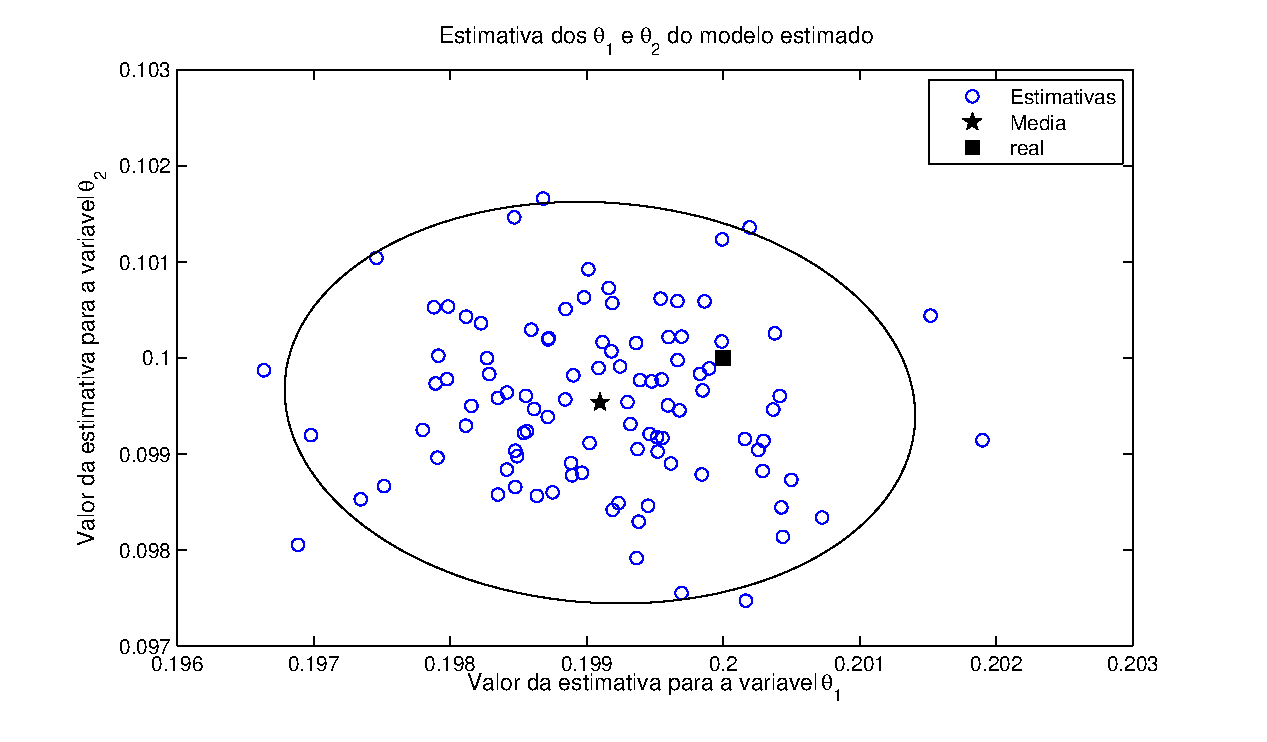
\includegraphics[width=0.9\columnwidth]{figures/rat_example2_a1_a2.eps}
	\caption{Estimativas obtidas nos 100 experimentos de Monte Carlo realizados para as vari�veis $\theta_1$ e
	$\theta_2$.}
	\label{fig:nl_rat_example2}
\end{figure}

Devido a presen�a de ru�do e ao erro de polariza��o apresentado ser menor que a vari�ncia do ru�do adicionado, sabe-se
que com o aumento de $N$ o valor de $\hat{\theta}_N \to \theta_0$.

%===============================================================================
\subsubsection{Sistemas originalmente racionais, quando $\mathcal{S} \notin \mathcal{M}$}
\label{sec:nl_si_algorithms_rationals_ex2}
%===============================================================================

Considere o sistema real:

\begin{equation}
y(t)=\frac{0.2 y(t-1)+0.1 y(t-1)u(t-1)+u(t-1)}{1+y^{2}(t-1)+y^{2}(t-2)}
\label{eq:nl_rat_exemple3}
\end{equation}

O sistema real $\mathcal{S}$ n�o consegue ser representada pela classe de modelos escolhida:

\begin{equation}
y(t)=\frac{\theta_1y(t-1)+\theta_2u(t-1)}{1+\theta_3y^{2}(t-1)+\theta_4y^{2}(t-2)}
\label{eq:nl_rat_exemple3_model}
\end{equation}

Utilizando par a simula��o um sinal PRBS de 635 pontos e um ru�do de vari�ncia $\sigma_e^2=0.005$ os resultados
da m�dia de 100 estimativas de Monte Carlo foram:

\begin{equation}
\theta_{\text{m�dia}} =\begin{bmatrix}
0.2279  &  1.1341  &  1.2716  &  1.3769
\end{bmatrix}
\nonumber
\end{equation}

%A vari�ncia encontrada foi de:
%
%\begin{equation}
%\theta_{\text{vari�ncia}} =1.0\times 10^{-3} \begin{bmatrix}
%0.0020  &  0.0535  &  0.3402  &	  0.3217
%\end{bmatrix}
%\nonumber
%\end{equation}

A fim de comparar a qualidade dos resultados obtidos, na Figura \ref{fig:nl_rat_example3} � apresentadas a resposta do
sistema real \eqref{eq:nl_rat_exemple3} e o sistema obtido pela estimativa utilizando o a classe de modelos
\eqref{eq:nl_rat_exemple3_model} para uma entrada do tipo degrau unit�rio.

\begin{figure}[htbp]
	\center
	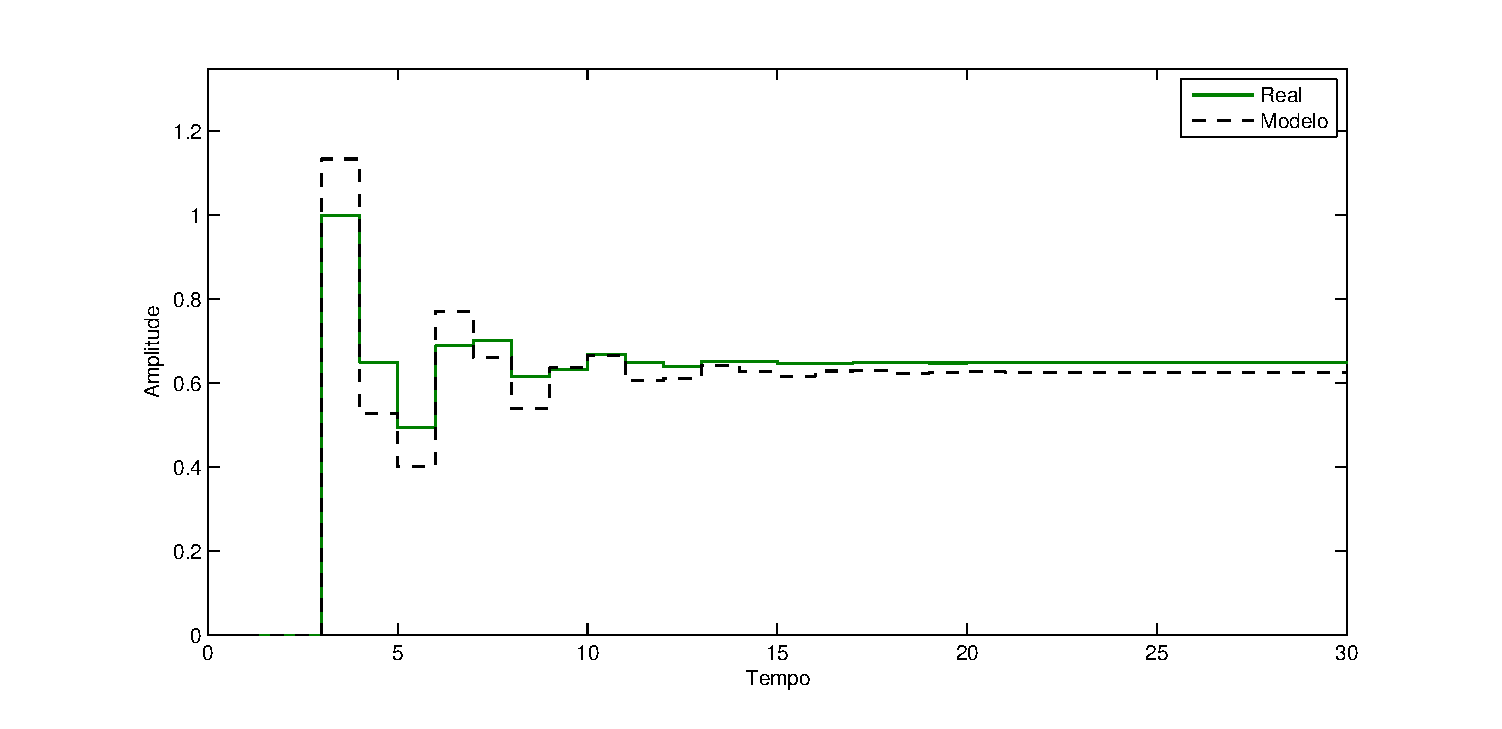
\includegraphics[width=0.9\columnwidth]{figures/rat_example3.eps}
	\caption{Exemplo 2 - Comparativo da resposta do sistema real e do modelo estimado para uma entrada do tipo degrau
	unit�rio}
	\label{fig:nl_rat_example3}
\end{figure}

O custo obtido para o modelo estimado foi de:

\begin{equation}
V(\theta)=1.1239
\nonumber
\end{equation}

Como n�o h� um valor de $\theta_0$ para compara��o, visto que o sistema real n�o consegue ser presentado pelo modelo,
optou-se por apresentar o resultado do sistema a uma resposta do tipo degrau unit�rio. Observa-se com isso que o sistema
estimado � apenas semelhante ao real, possuindo um sobrepasso maior e possuindo um ganho em regime ligeiramente
diferente que o sistema real. 
%===============================================================================
\subsubsection{Conversor CC-CC Buck}
\label{sec:nl_si_algorithms_rationals_buck}
% Aguirre 397
% Tese do corr�a - pg 27
%===============================================================================
O conversor de corrente cont�nua do tipo Buck possui um mapa n�o linear que pode ser obtido a partir da equa��o do
circuito apresentado na Figura \ref{fig:nl_models_buck_circuit} e que tem a forma como em: \cite{tse_buck}

\begin{equation}
y(t)=\alpha y(t-1)+\frac{h(d_n)^2 \beta E\left [ E-y(t-1) \right ]}{y(t-1)}
\label{eq:nl_alg_buck_circ}
\end{equation}
onde $\alpha = 0.8872$, $\beta = 1.2$ e $E=33$ s�o constantes que dependem apenas dos componentes do
circuito eletr�nico. $d_n$ � um sinal de tens�o que implementa a a��o de controle e a satura��o
$h(d_n)$ � dada por :

\begin{equation}
h(d_n)=\left\{\begin{matrix}
0 & \text{se } d_n < 0\\ 
1 & \text{se } d_n > 1\\ 
d_n & \text{caso contrario.}
\end{matrix}\right.
\nonumber
\end{equation}

\begin{figure}[htbp]
	\center
	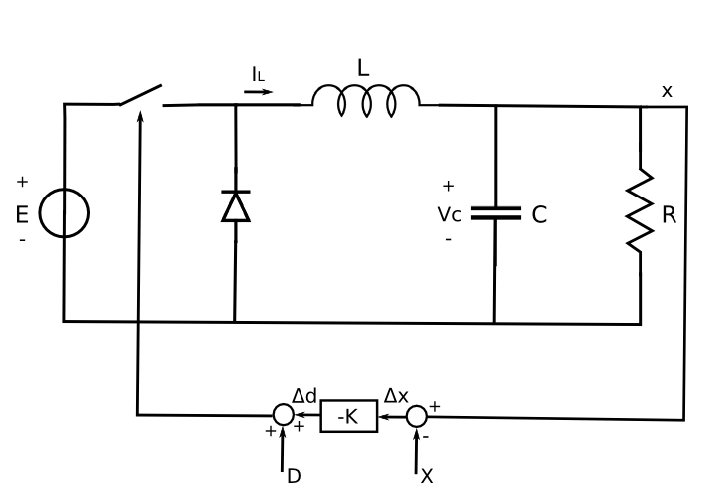
\includegraphics[width=0.55\columnwidth]{figures/nl_models_buck_circuit.eps}
	\caption{Circuito do conversor CC-CC Buck}
	\label{fig:nl_models_buck_circuit}
\end{figure}

Modelos polinomiais n�o resultam em bons modelos para a din�mica de \eqref{eq:nl_alg_buck_circ}. Um
modelo com estrutura {\it{ad rock}}, que aproxima relativamente bem a caracter�stica est�tica do
conversor �: \cite{aguirre_maps}

\begin{equation}
y(t)=O exp\left [ 22-y(t-1) \right ]+ \frac{a\; y(t-1)^2 -b\; y(t-1)+c}{y(t-1)}
\nonumber
\end{equation}
onde $O=46.429$, $a=2.6204$, $b=99.875$ e $c=1.4171\times 10^3$. Por outro lado a 

Para aplicar o algoritmo, escolhe-se inicialmente um modelo para o sistema em an�lise. O modelo
racional

\begin{equation}
y(t)=\frac{8.658+0.1223\times10^{-2}y(t-1)^3-0.441\times10^{-1}y(t-1)^2}
{1-0.8381\times10^{-1}y(t-1)+0.1766\times10^{-2}y(t-1)^2}
\label{eq:nl_alg_buck_rational}
\end{equation}
aproxima bem a din�mica em quest�o. \cite{aguirre}

Para a utiliza��o do algoritmo, escolheu-se um modelo com a forma:

\begin{equation}
y(t)=\frac{\theta_1+\theta_2y(t-1)^3+\theta_3(t-1)^2}{1+\theta_4y(t-1)+\theta_5y(t-1)^2}
\label{eq:nl_alg_buck_rational_model}
\end{equation}

Os par�metros da equa��o \eqref{eq:nl_alg_buck_rational} s�o os valores de refer�ncia para a utiliza��o do
m�todos descrito em \cite{aguirre}. Utilizando o algoritmo previamente apresentado, o resultado da estimativa
foi:

\begin{equation}
\theta =\begin{bmatrix}
8.8807 & 8.6698\times 10^{-4} &-0.0359 &-0.0736 & 0.0013 
\end{bmatrix}
\nonumber
\end{equation}

Como pode ser observado, pelos resultados de $\theta$ obtidos e os valores esperados, existe polariza��o na
estimativa obtida. Isso em parte se d� pela falta de capacidade da classe de modelos escolhida em representar
o processo real e pela escolha do modelo de ru�do que para este caso foi apenas utilizado o erro da
estimativa, com rela��o a sa�da do sistema real obtido.

Foram utilizadas amostras de 100 pontos para esta estimativa e realizados 100 experimentos de Monte Carlo.
Os resultados obtidos foram de uma m�dia de:

\begin{equation}
\text{m�dia de }\;\theta =\begin{bmatrix}
8.8976  &    8.6762\times 10^{-4}    & -0.0360 &  -0.0736  &  0.0013
\end{bmatrix}
\nonumber
\end{equation}

com uma covari�ncia de 

\begin{equation}
\theta_{\text{Covari�ncia}} = 1.0\times 10^{-3}\begin{bmatrix}
 0.4842 &  0.0000 & -0.0011 &  0.0007 &-0.0000 \\
 0.0000 &  0.0000 & -0.0000 & -0.0000 & 0.0000 \\
-0.0011 & -0.0000 &  0.0000 & -0.0000 & 0.0000 \\
 0.0007 & -0.0000 & -0.0000 &  0.0000 &-0.0000 \\
-0.0000 &  0.0000 &  0.0000 & -0.0000 & 0.0000 
\end{bmatrix}
\nonumber
\end{equation}


%===============================================================================
\section{Considera��es Finais}
\label{sec:nl_conclusions}
%===============================================================================


%===============================================================================


%===============================================================================
\chapter{Controle baseado em dados}
\label{chapter:vfrt}
%===============================================================================

Neste cap�tulo tem-se o objetivo de introduzir a id�ia de projeto de controladores baseado em dados, a ideia de
refer�ncia virtual e o uso disso em conjunto para a identifica��o de controladores n�o lineares.

Inicialmente na se��o \ref{sec:vrft_control_data_based} ser� introduzido o conceito de projeto de controlaodres baseados
em dados. Alguns dos principais m�todos e suas subdivis�es em m�todos diretos: onde n�o existe a necessidade de
identifica��o da planta, para ent�o identificar o controlador; m�todos iterativos: onde a cada conjunto de dados
coletados da planta um novo controlador � encontrado e aplicado sobre a planta at� que se convirja para o valor m�nimo
da fun��o custo.

Deseja-se adicionar um enfoque ao m�todo direto que utiliza refer�ncia virtual: VRFT (se��o \ref{sec:vrft_vrft}).
Quer-se com isso introduzir e exeplificar a utiliza��o de refer�ncia virtual para a obten��o dos sinais necess�rios para
a identifica��o do controlador ideal para este sistema.

Na se��o \ref{sec:vrft_nonlinear} introduz-se a id�ia de utiliza��o de m�todos de projeto de controladores baseados em
dados, juntamente com a utilzia��o de refer�ncia virtual para a obten��o dos sinais necess�rios. Esta se��o utiliza o
algoritmo apresentado na se��o \ref{sec:nl_si_algorithms_rationals} para identifica��o de sistemas n�o lineares que
podem ser descritos por classes de modelos NARMAX polinomiais ou racionais. Alguns exemplos ser�o apresentados para que
se possa avaliar a qualidade das estimativas obtidas.

Ao fim, na se��o \ref{sec:vrft_conclusions}, ser�o apresentadas as considera��es finais a respeito do que foi visto
neste capitulo.



%===============================================================================
%===============================================================================
\section{Defini��es}
\label{sec:vrft_control_data_based}
%===============================================================================
O projeto de controladores baseados em dados consiste em obter, ou estimar, os par�metros de uma fam�lia ou conjunto de 
modelos baseados nos dados obtidos da planta sob an�lise. Os dados utilizados para esta tarefa s�o usualmente os sinais
de entrada e sa�da do sistema.

Como j� foi discutido na se��o (\ref{sec:si_project_experiments}) estes dados podem ser obtidos de
diversas formas. Algumas vezes estas informa��es podem vir da opera��o normal da planta em malha
fechada com a presen�a de algum controlador. Situa��o esta que tem um grande apelo em plantas
industriais, onde a parada do processo, para levantamento de informa��es, � indesej�vel e muitas
vezes at� invi�vel. Se existe a possibilidade de parar a planta e aplicar sinais predeterminados,
o projeto de experimentos pode trazer muitas vantagens (se��o \ref{sec:si_project_experiments}).

O projeto de controladores baseados em dados consiste em estimar os parametros da estrutura do controlador usando os
dados de entrada e sa�da coletados do sistema. A estimativa � feita de forma direta, ou seja, sem a necessidade de um
passo intermedi�rio para identifica��o da planta do processo. \cite{eckard_campestrini}

% http://www.sciencedirect.com/science/article/pii/S0005109808002288
Several data-based control design methods explicitly optimizing performance criteria have appeared in the literature,
with different approaches and for different performance criteria. These criteria express either one or a combination  of
the fundamental control objectives: reference tracking, noise rejection, and economic use of control energy. In Kammer,
Bitmead, and Bartlett (2000) an iterative procedure based on spectral analysis, named Frequency Domain Tuning (FDT), 
has been proposed for the minimization of an H2 performance criterion for a system with zero reference; hence, no
tracking objective is pursued. The Virtual Reference Feedback Tuning (VRFT) method ( [Campi et al., 2002] and [Campi
and Savaresi, 2006]) is based on a clever manipulation of variables which transforms an H2 performance criterion into
one which is quadratic in the design parameters. The resulting quadratic cost function can be minimized directly, so
that no iterations are required. However, only the reference tracking objective is treated (unless a two degree of
freedom controller is used, as in Lecchini, Campi, and Savaresi (2002)) and the global minimum of the resulting
quadratic function coincides with that of the original criterion only under ideal conditions. Not suffering from this
second limitation, but again an iterative procedure, is Correlation-based Tuning (CbT) ( [Karimi et al., 2003] and
[Karimi et al., 2004]), which uses instrumental variable ideas to eliminate the deleterious effect of noise on the
achievement of its reference tracking objective. Data-based optimization of a general H2 performance criterion appears
in Hjalmarsson, Gunnarsson, and Gevers (1994). There, a method for obtaining an unbiased estimate of the gradient of
the cost function directly from closed-loop data is proposed; this method has been named Iterative Feedback Tuning
(IFT). IFT is discussed in depth in Hjalmarsson, Gevers, Gunnarsson, and Lequin (1998), Hjalmarsson (2002) and extended
in Proch�zka, Gevers, Anderson, and Ferrera (2005) to even more general performance criteria, which contain robustness
enhancement objectives.
\cite{Bazanella_h2criteria2008} 

Seja a esperan�a de um valor $E\left [ \cdot \right ]$ definido por: \cite{ljung}

\begin{equation}
\bar{E}\left [ f(t) \right ]\equiv \lim_{N \to \infty } \frac{1}{N}\sum_{t=1}^{N}E\left [ f(t)
\right]
\label{eq:vrft_db_hope}
\end{equation}

O ru�do � um processo quasi-estacion�rio, que pode ser descrito como $\nu(t)=H_0(z)e(t)$, onde
$e(t)$ � ru�do branco com vari�ncia $\sigma_e^2$. Ambas fun��es de transfer�ncia, $G_0(z)$ e $H_0(z)$,
s�o racionais e causais. Assume-se que $H(\infty)=1$, ou seja, a resposta impulsiva do filtro
$H_0(z)$ satisfaz $h(0)=1$. \cite{campestrini}

Na Figura (\ref{fig:vrft_db_control_loop}) � apresentado um usual sistema com realimenta��o de sa�da onde s�o
destacados os blocos do controlador, da planta e da fun�a� que modifica o ru�do branch $e(t)$.

\begin{figure}[htbp]
\center
% Generated with LaTeXDraw 2.0.8
% Tue Jun 05 22:30:25 BRT 2012
% \usepackage[usenames,dvipsnames]{pstricks}
% \usepackage{epsfig}
% \usepackage{pst-grad} % For gradients
% \usepackage{pst-plot} % For axes
\scalebox{1} % Change this value to rescale the drawing.
{
\begin{pspicture}(0,-2.0492187)(9.84,2.0692186)
\pscircle[linewidth=0.04,dimen=outer](1.401875,-1.0292188){0.2}
\psframe[linewidth=0.04,dimen=outer](4.401875,-0.62921876)(2.601875,-1.4292188)
\psframe[linewidth=0.04,dimen=outer](7.201875,-0.62921876)(5.601875,-1.4292188)
\pscircle[linewidth=0.04,dimen=outer](8.401875,-1.0292188){0.2}
\psline[linewidth=0.04cm,arrowsize=0.05291667cm 2.0,arrowlength=1.4,arrowinset=0.4]{->}(0.001875,-1.0292188)(1.201875,-1.0292188)
\psline[linewidth=0.04cm,arrowsize=0.05291667cm 2.0,arrowlength=1.4,arrowinset=0.4]{->}(1.601875,-1.0292188)(2.601875,-1.0292188)
\psline[linewidth=0.04cm,arrowsize=0.05291667cm 2.0,arrowlength=1.4,arrowinset=0.4]{->}(4.401875,-1.0292188)(5.601875,-1.0292188)
\psline[linewidth=0.04cm,arrowsize=0.05291667cm 2.0,arrowlength=1.4,arrowinset=0.4]{->}(7.201875,-1.0292188)(8.201875,-1.0292188)
\psline[linewidth=0.04cm,arrowsize=0.05291667cm 2.0,arrowlength=1.4,arrowinset=0.4]{->}(8.4,0.16921872)(8.401875,-0.82921875)
\psline[linewidth=0.04cm,arrowsize=0.05291667cm 2.0,arrowlength=1.4,arrowinset=0.4]{->}(8.601875,-1.0292188)(9.801875,-1.0292188)
\psline[linewidth=0.04cm,arrowsize=0.05291667cm 2.0,arrowlength=1.4,arrowinset=0.4]{<-}(1.401875,-1.2292187)(1.401875,-2.0292187)
\psline[linewidth=0.04cm](1.401875,-2.0292187)(9.201875,-2.0292187)
\psline[linewidth=0.04cm](9.201875,-2.0292187)(9.201875,-1.0292188)
\usefont{T1}{ptm}{m}{n}
\rput(1.0771874,-0.7192188){+}
\usefont{T1}{ptm}{m}{n}
\rput(8.0771885,-0.7192188){+}
\usefont{T1}{ptm}{m}{n}
\rput(8.0771885,-1.3192188){+}
\usefont{T1}{ptm}{m}{n}
\rput(1.6265626,-1.3192188){-}
\usefont{T1}{ptm}{m}{n}
\rput(0.441875,-0.7292188){\small $r(t)$}
\usefont{T1}{ptm}{m}{n}
\rput(3.561875,-1.0292188){\small $C(z, \rho)$}
\usefont{T1}{ptm}{m}{n}
\rput(6.331875,-1.0492188){\small $G_0(z)$}
\usefont{T1}{ptm}{m}{n}
\rput(5.081875,-0.7292188){\small $u(t)$}
\usefont{T1}{ptm}{m}{n}
\rput(1.941875,-0.7292188){\small $\varepsilon (t)$}
\usefont{T1}{ptm}{m}{n}
\rput(7.851875,-0.20921877){\small $\nu(t)$}
\usefont{T1}{ptm}{m}{n}
\rput(9.271875,-0.7292188){\small $y(t)$}
\psframe[linewidth=0.04,dimen=outer](9.201875,0.9707812)(7.601875,0.17078124)
\usefont{T1}{ptm}{m}{n}
\rput(8.331875,0.55078125){\small $H_0(z)$}
\psline[linewidth=0.04cm](8.4,0.96921873)(8.4,1.5692188)
\usefont{T1}{ptm}{m}{n}
\rput(8.271875,1.8707812){\small $e(t)$}
\end{pspicture} 
}
\caption{Sistema de controle em malha fechada, com presen�a do sinal de ru�do.}
\label{fig:vrft_db_control_loop}
\end{figure}

A equa��o \eqref{eq:vrft_db_closed_loop} descreve a rela��o entre entrada e sa�da do sistema
apresentado na Figura (\ref{fig:vrft_db_control_loop}).

\begin{equation}
T(z, \rho)=\frac{C(z,\rho)G_0(z)}{1+C(z,\rho)G_0(z)}
\label{eq:vrft_db_closed_loop}
\end{equation}

Controle baseado em dados pode ser dividido em dois grupos principais: m�todos iterativos onde
experimentos s�o realizados sobre o sistema atualizando-se o controlador, o processo ent�o � repetido
at� que se atinja um valor minimo para a fun��o custo deste sistema. O segundo grupo � o de m�todos
n�o iterativos, onde apenas com um experimento, ou um conjunto de dados, os par�metros do
controlador s�o estimados.

%===============================================================================
\subsection{Iterative feedback tuning}
\label{sec:vrft_control_ift}
%===============================================================================

O m�todo IFT utiliza um algoritmo iterativo para minimizar uma fun��o custo $H_2$. O m�todo
considera que o sistema � controlado por um controlador com dois graus de liberdade:

\begin{equation}
u(t)=C_r(z)r(t)-C_y(z)y(t)
\label{eq:vrft_db_ift_controller}
\end{equation}

Na Figura (\ref{fig:vrft_db_ift}) � apresentado a organiza��o dos blocos dos controladores
de \eqref{eq:vrft_db_ift_controller}, $C_r(z)$ e $C_y(z)$. O controlador pode ser
entendido como o conjunto destes dois:\cite{ift_theory_and_applications}

\begin{equation}
C(z) \equiv  \left \{ C_r(z),\, C_y(z)  \right \} 
\nonumber
\end{equation}

\begin{figure}[htbp]
\center
\scalebox{1} % Change this value to rescale the drawing.
{
\begin{pspicture}(0,-1.68)(9.48,1.72)
\usefont{T1}{ptm}{m}{n}
\rput(7.691875,1.5215625){\small $\nu(t)$}
\pscircle[linewidth=0.04,dimen=outer](4.0,0.32){0.2}
\pscircle[linewidth=0.04,dimen=outer](8.0,0.32){0.2}
\psframe[linewidth=0.04,dimen=outer](6.8,0.72)(5.2,-0.08)
\psframe[linewidth=0.04,dimen=outer](2.8,0.72)(1.2,-0.08)
\psframe[linewidth=0.04,dimen=outer](6.8,-0.88)(5.2,-1.68)
\psline[linewidth=0.04cm,arrowsize=0.05291667cm 2.0,arrowlength=1.4,arrowinset=0.4]{->}(0.0,0.32)(1.2,0.32)
\psline[linewidth=0.04cm,arrowsize=0.05291667cm 2.0,arrowlength=1.4,arrowinset=0.4]{->}(2.8,0.32)(3.8,0.32)
\psline[linewidth=0.04cm,arrowsize=0.05291667cm 2.0,arrowlength=1.4,arrowinset=0.4]{->}(4.2,0.32)(5.2,0.32)
\psline[linewidth=0.04cm,arrowsize=0.05291667cm 2.0,arrowlength=1.4,arrowinset=0.4]{->}(6.8,0.32)(7.8,0.32)
\psline[linewidth=0.04cm,arrowsize=0.05291667cm 2.0,arrowlength=1.4,arrowinset=0.4]{->}(8.2,0.32)(9.2,0.32)
\psline[linewidth=0.04cm,arrowsize=0.05291667cm 2.0,arrowlength=1.4,arrowinset=0.4]{<-}(6.8,-1.28)(8.0,-1.28)
\psline[linewidth=0.04cm](8.0,-1.28)(8.0,0.12)
\psline[linewidth=0.04cm,arrowsize=0.05291667cm 2.0,arrowlength=1.4,arrowinset=0.4]{<-}(4.0,0.12)(4.0,-1.28)
\psline[linewidth=0.04cm](4.0,-1.28)(5.2,-1.28)
\usefont{T1}{ptm}{m}{n}
\rput(8.911875,0.5215625){\small $y(t)$}
\usefont{T1}{ptm}{m}{n}
\rput(0.481875,0.5215625){\small $r(t)$}
\usefont{T1}{ptm}{m}{n}
\rput(1.901875,0.3215625){\small $C_r(z)$}
\usefont{T1}{ptm}{m}{n}
\rput(5.951875,0.3215625){\small $G_0(z)$}
\usefont{T1}{ptm}{m}{n}
\rput(5.931875,-1.2784375){\small $C_y(z)$}
\usefont{T1}{ptm}{m}{n}
\rput(4.721875,0.7215625){\small $u(t)$}
\psline[linewidth=0.04cm,arrowsize=0.05291667cm 2.0,arrowlength=1.4,arrowinset=0.4]{->}(8.0,1.32)(8.0,0.52)
\usefont{T1}{ptm}{m}{n}
\rput(4.2592187,0.1315625){-}
\end{pspicture} 
}
\caption{Diagrama de bloco do sistema utilizado na identifica��o IFT.}
\label{fig:vrft_db_ift}
\end{figure}

A fun��o custo utilizada como crit�rio no m�todo � apresentada em \eqref{eq:vrft_db_ift_j_cost}. 

\begin{equation}
J(\rho)=\frac{1}{2N}E\left [ \sum_{t=1}^{N}(L_y \tilde{y}_t(\rho))^2 +\lambda  \sum_{t=1}^{N}(L_u
u_t(\rho))^2 \right ]
\label{eq:vrft_db_ift_j_cost}
\end{equation}

O primeiro termo em \eqref{eq:vrft_db_ift_j_cost} � o erro entre a resposta obtida e a resposta
desejada, balanceada por um filtro $L_y$ a segunda parte � o custo de controle balanceado pelo
filtro $L_u$. Com $T_0(\rho)$ e $S_0(\rho)$ sendo a fun��o de transfer�ncia em malha fechada e a
fun��o sensibilidade, respectivamente:


\begin{equation}
T_0(\rho)=\frac{C_r(\rho)G_0}{1+C_y(\rho)G_0}
\nonumber
\end{equation}

\begin{equation}
S_0(\rho)=\frac{1}{1+C_y(\rho)G_0}
\nonumber
\end{equation}

E sendo $r$ e $\nu$ independentes, \eqref{eq:vrft_db_ift_j_cost} pode ser rescrito como
\eqref{eq:vrft_db_ift_j_cost_parts}

\begin{equation}
J(\rho)=\frac{1}{2N}\sum_{t=1}^{N}\left \{ L_y(T_d r-T_0(\rho)r) \right \}^2+\frac{1}{2} E\left [ \left \{ L_y S_0(\rho) \nu \right \}^2 \right ]
+ \lambda \frac{1}{2N}E\left [ \sum_{t=1}^{N}(L_u u_t(\rho))^2 \right ]
\label{eq:vrft_db_ift_j_cost_parts}
\end{equation}

Onde o primeiro termo � o erro de seguimento de refer�ncia, o segundo � a contribui��o do dist�rbio
e o terceiro � o esfor�o de controle.

Para minimizar \eqref{eq:vrft_db_ift_j_cost_parts}, busca-se encontrar um ponto
estacion�rio da equa��o, para isso calcula-se o gradiente desta equa��o e aplica-se o
algoritmo para a converg�ncia apresentado em \eqref{eq:vrft_db_ift_algoritm}.
\cite{hajalmson_ift_non_linear}

\begin{equation}
\rho_{i+1}=\rho_i - \gamma_i R_i^{-1}\frac{\partial J}{\partial \rho}(\rho_i)
\label{eq:vrft_db_ift_algoritm}
\end{equation}

$R_i$ � uma matriz positiva definida, tipicamente uma estimativa da Hessiana de $J$, como por
exemplo a aproxima��o de Gauss-Newton.

Para cada itera��o $i$ em \eqref{eq:vrft_db_ift_algoritm}, o m�todo IFT necessita de dois
experimentos, cada um de tamanho $N$. 


% ===============================================================================
\section{Virtual reference feedback tuning}
\label{sec:vrft_vrft}
% ===============================================================================

% Em aplica��es pr�ticas, a descri��o matem�tica da planta n�o � dispon�vel e o sistema deve ser identificado
% baseado nas medidas obtidas deste sistema. Este assunto tem atra�do a aten��o de diversos engenheiros de
% controle desde 1940 com o pioneiro trabalho de Ziegler e Nichols (1942) com ajuste de controladores PID
% industriais. Depois do trabalho de Ziegler e Nichols diversos trabalhos surgiram, muitos em formas de
% aperfei�oamento e extens�es das t�cnicas j� apresentadas, e algumas com desenvolvimentos em novas dire��es
% (\cite{mcmillan1983tuning}, \cite{Haalman1965}). A caracter�stica principal destes m�todos � que eles podem
% ser facilmente utilizados: simples experimentos sobre a planta s�o executados e simples regras 
% s�o aplicadas sobre os dados obtidos. \cite{campi_leccini_savaresi2002}


VRFT do ingl�s {\it{Virtual reference feedback tuning}} � um m�todo direto para identifica��o de
controladores, ou seja, n�o � necess�rio o conhecimento ou identifica��o da planta para que este m�todo seja
utilizado. O m�todo se baseia na utiliza��o de apenas um conjunto de dados, n�o necessitando de experimentos
espec�ficos. O procedimento procura pelo ponto �timo do crit�rio escolhido para a identifica��o do controlador.
\cite{campi_savaresi2000}

Diferentemente de m�todos iterativos, o VRFT n�o recai sobre m�nimos locais, sempre procurando o m�nimo
global do crit�rio escolhido, sob condi��es ideais. Ele ir� buscar o m�nimo da fun��o custo dentro das limita��es de
excitabilidade do sinal utilizado. Se o sinal utilizado para exitar o sistema for suficientemente informativo, ent�o o
minimo encontrado pelo m�todo ser� um minimo global.

Assume-se que a planta do sistema � {\it{linear}} SISO ({\it{single input single output}}) de tempo discreto,
descrito pela fun��o de transfer�ncia racional $G_0(z)$. Tal que esta fun��o de transfer�ncia � desconhecida e
tem-se apenas acesso ao conjunto de dados coletados do experimento. \cite{campi_leccini_savaresi2002}

O controlador a ser identificado pode ser parametrizado como abaixo:

\begin{equation}
C(z,\theta)=\beta^T(z)\theta
\label{eq:vrft_method_controller}
\end{equation}

Onde $\beta(z) = \left [ \beta_1(z)\;\; \beta_2(z)\;\; \cdots \;\; \beta_n(z)\right ]^T$ � um vetor
linear de fun��es de transfer�ncias de tempo discreto e $\theta = \left [ \vartheta_1 \;\;
\vartheta_2 \;\; \cdots \;\; \vartheta_n \right ]^T \in \mathcal{R}^n$ � um vetor $n$-dimensional de
par�metros a serem estimados.

O problema de identifica��o do controlador consiste em encontrar um $\hat{\theta}$ que minimize o
crit�rio performance \eqref{eq:vrft_method_cost_func} que � dependente do modelo de refer�ncia
escolhido.

\begin{equation}
J_{MR}(\theta) = \left \| \left ( \frac{G(z)C(z,\theta)}{1+G(z)C(z,\theta)} -M(z) \right )W(z)
\right \|_2^2 
\label{eq:vrft_method_cost_func}
\end{equation} 

Sendo $M(z)$ o modelo de refer�ncia a ser atingido em malha fechada quando o controlador
obtido � aplicado sobre a planta e $W(z)$ � uma matriz para pondera��o escolhida pelo usu�rio.

M�todos diretos s�o conceitualmente mais naturais que os indiretos, mas mesmo com o apelo que possuem,
apenas alguns m�todos genuinamente diretos s�o encontrados na literatura, dois destes s�o VRFT e IFT, mesmo
estes dois m�todos pertencendo uma a mesma classe, algumas diferen�as s�o ressaltadas: \cite{campi_savaresi2000}

\begin{itemize}
	\item {\it{IFT}} � baseado em um m�todos de gradiente decrescente e al�m disso � uma t�cnica
	iterativa. Usualmente este m�todo converge para o minimo local mais pr�ximo das condi��es iniciais.
	Ele requer experimentos espec�ficos sobre a planta, com entradas especificas.
	\item {\it{VRFT}} � um procedimento n�o iterativo que procura pelo minimo global do crit�rio de
	performance \eqref{eq:vrft_method_cost_func}. Este m�todo n�o requer experimentos espec�ficos sobre
	a planta, podendo inclusive utilizar os dados do funcionamento normal da planta.
\end{itemize}

%===============================================================================
\subsection{O m�todo}
\label{sec:vrft_framework}
%===============================================================================

Nesta se��o ser� apresentado uma breve descri��o de como funciona o algoritmo para obten��o do controlador
utilizando o m�todo VRFT. Para maiores detalhes e discuss�es aprofundadas � indicada a leitura de
\cite{campi_savaresi2000, campi_leccini_savaresi2002, campestrini_nonminumum_phase}.

Suponha que o controlador $C(z, \theta)$ resulta um sistema em malha fechada cuja fun��o de
transfer�ncia � dada por $M(z)$. Desta forma, se $M(z)$ for excitado com qualquer sinal $r(t)$,
sua sa�da ser� $M(z)r(t)$. Uma premissa para que o sistema em malha fechada tenha a mesma
fun��o de transfer�ncia que o modelo de refer�ncia � que a sa�da dos dois seja a mesma para um dado
sinal $\bar{r}(t)$.

Baseado no sinal medido $y(t)$, considera-se um sinal $\bar{r}(t)$ tal que $M(z)\bar{r}(t)=y(t)$.
Esta refer�ncia � conhecida como {\it{virtual}} pois ela n�o existe e n�o foi utilizada para gerar o
sinal $y(t)$. A figura (\ref{fig:vrft_method_cl}) apresenta o sistema em malha fechada e os sinais
utilizados.

\begin{figure}[htbp]
\center
%\scalebox{1} % Change this value to rescale the drawing.
%{
\begin{pspicture}(0,-1.4292188)(9.02,1.4692187)
\pscircle[linewidth=0.04,linestyle=dashed,dash=0.16cm 0.16cm,dimen=outer](1.4,0.97078127){0.2}
\psframe[linewidth=0.04,linestyle=dashed,dash=0.16cm 0.16cm,dimen=outer](4.8,1.3707813)(3.0,0.57078123)
\psframe[linewidth=0.04,dimen=outer](7.6,1.3707813)(6.0,0.57078123)
\psline[linewidth=0.04cm,arrowsize=0.05291667cm 2.0,arrowlength=1.4,arrowinset=0.4]{->}(0.0,0.97078127)(1.2,0.97078127)
\psline[linewidth=0.04cm,linestyle=dashed,dash=0.16cm 0.16cm,arrowsize=0.05291667cm 2.0,arrowlength=1.4,arrowinset=0.4]{->}(1.6,0.97078127)(3.0,0.97078127)
\psline[linewidth=0.04cm,arrowsize=0.05291667cm 2.0,arrowlength=1.4,arrowinset=0.4]{->}(4.8,0.97078127)(6.0,0.97078127)
\psline[linewidth=0.04cm](7.6,0.97078127)(9.0,0.97078127)
\psline[linewidth=0.04cm,linestyle=dashed,dash=0.16cm 0.16cm,arrowsize=0.05291667cm 2.0,arrowlength=1.4,arrowinset=0.4]{<-}(1.4,0.7707813)(1.4,-0.02921875)
\psline[linewidth=0.04cm,linestyle=dashed,dash=0.16cm 0.16cm](1.4,-0.02921875)(8.4,-0.02921875)
\psline[linewidth=0.04cm,linestyle=dashed,dash=0.16cm 0.16cm](8.4,-0.02921875)(8.4,0.97078127)
\usefont{T1}{ptm}{m}{n}
\rput(1.1126562,1.2807813){+}
\usefont{T1}{ptm}{m}{n}
\rput(1.6473438,0.68078125){-}
\usefont{T1}{ptm}{m}{n}
\rput(0.47,1.2707813){\small $\bar{r}(t)$}
\usefont{T1}{ptm}{m}{n}
\rput(3.99,0.97078127){\small $C(z, \rho)$}
\usefont{T1}{ptm}{m}{n}
\rput(6.76,0.9507812){\small $G_0(z)$}
\usefont{T1}{ptm}{m}{n}
\rput(5.51,1.2707813){\small $u(t)$}
\usefont{T1}{ptm}{m}{n}
\rput(2.25,1.2707813){\small $\varepsilon (t)$}
\usefont{T1}{ptm}{m}{n}
\rput(8.3,1.2707813){\small $y(t)$}
\psframe[linewidth=0.04,dimen=outer](6.0,-0.62921876)(3.8,-1.4292188)
\usefont{T1}{ptm}{m}{n}
\rput(4.91,-1.0492188){\small $M^{-1}(z)$}
\psline[linewidth=0.04cm](9.0,0.97078127)(9.0,-1.0292188)
\psline[linewidth=0.04cm](9.0,-1.0292188)(6.0,-1.0292188)
\psline[linewidth=0.04cm](3.8,-1.0292188)(0.0,-1.0292188)
\psline[linewidth=0.04cm](0.0,-1.0292188)(0.0,0.97078127)
\end{pspicture} 
%}
\caption{Diagrama de blocos para o m�todo VRFT. S�o destacados os sinais reais $u(t)$ e $y(t)$ al�m dos sinais virtuais
$\varepsilon (t)$ e $\bar{r}(t)$.}
\label{fig:vrft_method_cl}
\end{figure}

O sinal $\varepsilon(t)$ � o erro entre os sinais $y(t)$ e $\bar{r}(t)$. Sabe-se que quando a planta �
excitada com o sinal $u(t)$, o sinal $y(t)$ � obtido. Analogamente para um controlador, quando este �
excitado com o sinal $\varepsilon(t)$, o sinal $u(t)$ � obtido. A tarefa do m�todo VRFT � encontrar este
controlador, como os sinais $u(t)$ e $\varepsilon(t)$ s�o conhecidos, a tarefa reduz-se a um problema de
identifica��o. Comumente, usa-se um pr�-filtro nos dados coletados. A ideia principal do uso deste
filtro ser� explicada posteriormente na se��o (\ref{sec:vrft_framework_filter}). 

O algoritmo pode ser descrito pelos passos a seguir \cite{campi_savaresi2000}:

\begin{enumerate}
	\item Filtram-se os sinais de entrada e sa�da com algum filtro $L(z)$:

\begin{equation}
y_L (t)=L(z)y(t), \;\;\; u_L (t)=L(z)u(t) 
\label{eq:vrft_method_algorithm_filter_io}
\end{equation}

\item Encontra-se um sinal de refer�ncia $\bar{r}_L (t)$ no qual a sa�da do modelo de refer�ncia
$M(z)$ seja exatamente $y_L (t)$ quando alimentado pelo sinal:

\begin{equation}
y_L (t)=M(z) \bar{r}_L (t)
\label{eq:vrft_method_algorithm_ref}
\end{equation}

\item Selecione o vetor de par�metros do controlador $\hat{\theta}$ que minimize o crit�rio
\eqref{eq:vrft_method_algorithm_criter}

\begin{equation}
J_{VR}^N(\theta)=\frac{1}{N}\sum_{t=1}^{N}(u_L(t)-\varphi_L^T(t)\theta)^2
\label{eq:vrft_method_algorithm_criter}
\end{equation}

\begin{equation}
\varphi_L(t)=\beta(z)e_L(t)
\nonumber
\end{equation}

Desde que \eqref{eq:vrft_method_algorithm_criter} seja quadr�tica em $\theta$ o vetor de par�metros
$\hat{\theta}$ que minimiza esta fun��o custo pode ser calculado por:

\begin{equation}
\hat{\theta}= \left [ \sum_{t=1}^{N}\varphi_L(t) \varphi_L(t)^T\right ]^{-1}
\sum_{t=1}^{N}\varphi_L(t) u_L(t)
\label{eq:vrft_method_algorithm_result}
\end{equation}

\end{enumerate}

%===============================================================================
\subsubsection{Filtro $L(z)$}
\label{sec:vrft_framework_filter}
%===============================================================================

Considerando a fun��o custo $J_{MR}(\theta)$ apresentada em \eqref{eq:vrft_method_cost_func} e o
crit�rio do m�todo de refer�ncia virtual $J_{VR}(\theta)$ apresentado em
\eqref{eq:vrft_method_algorithm_criter} serem diferentes. A escolha correta do filtro $L(z)$
propicia que estas duas equa��es tenham m�nimos muito pr�ximos.
\cite{campi_leccini_savaresi2002}

A utiliza��o do filtro � de grande import�ncia em situa��es onde a escolha do modelo $\mathcal{C}(z,
\theta)$ n�o consegue representar a totalidade do controlador �timo ($C_0(z)$) que quando aplicado em conjunto com a
planta proporciona a exata resposta desejada pela escolha de $M(z)$.

\begin{equation}
C_0(z) \notin \mathcal{C}(z, \theta)
\nonumber
\end{equation}

O crit�rio $J_{MR}(\theta)$ pode ser reescrito utilizando-se o controlador �timo $C_0(z)$ como em:

\begin{equation}
J_{MR}(\theta)= \frac{1}{2\pi} \int_{-\pi}^{\pi} \frac{\left | G \right |^2 \left | W \right |^2 }
{\left | 1+GC(\theta) \right |^2} 
\frac{\left |C(\theta)-C_0  \right |^2}{\left |1+GC_0 \right |^2}d\omega 
\label{eq:vrft_method_filter_cost_func}
\end{equation}

Considerando que $J_{VR}^N$ seja conhecido, quando a quantidade de dados cresce: $N \to \infty$
tem-se \eqref{eq:vrft_method_filter_criter_assim}. 

\begin{equation}
J_{VR}^N(\theta) \to J_{VR}(\theta = E \left [ (u_L(t) - C(z, \theta)\varepsilon_L(t))^2\right ])
\label{eq:vrft_method_filter_criter_assim}
\end{equation}

Utilizando as defini��es de $u_L(t)$, $\varepsilon_L(t)$ e dada a defini��o de $C_0(z)$ juntamente com o
teorema de Perseval \cite{ljung}, o crit�rio assint�tico \eqref{eq:vrft_method_filter_criter_assim}
tem sua representa��o como em:

\begin{equation}
J_{VR}(\theta)= \frac{1}{2\pi} \int_{-\pi}^{\pi} \left | G \right |^2 \left | C(\theta)-C_0 \right
|^2 \left | 1-M \right |^2 \frac{\left | L \right |^2}{\left | M \right |^2} \Phi_u \; d\omega
\label{eq:vrft_method_filter_criter_vr}
\end{equation}

Onde $\Phi_u $ � a densidade do espectro do sinal $u(t)$.

Para o caso onde $C_0 \in C(z, \theta)$ a escolha de $L(z)$ n�o afeta o resultado, usualmente
escolhe-se ent�o $L(z)=1$. Caso o controlador n�o consiga ser representado pelo modelo, a escolha de
$L(z)$ pode ser feita por:\cite{campi_leccini_savaresi2002}

\begin{equation}
\left | L \right | ^2 = \left | 1-M \right | ^2 \left | M \right | ^2 \left | W \right | ^2 \frac{1}
{\Phi_u}, \;\;\; \forall \omega \in [-\pi; \pi].
\label{eq:vrft_method_filter_l}
\end{equation}

Obt�m-se com a utiliza��o do filtro, uma estimativa onde o erro de polariza��o � minimizado.
%===============================================================================
\subsubsection{Dados corrompidos por ruido}
\label{sec:vrft_framework_noise}
%===============================================================================

Todos os equacionamentos at� aqui apresentados consideraram que o sistema n�o fosse afetado por
ru�do. Nesta se��o ser� apresentado brevemente o comportamento do m�todo quando o sinal $y(t)$ �
corrompido por um ruido aditivo como:

\begin{equation}
\tilde{y}(t)=G_0(z)u(t) + \nu(t)
\label{eq:vrft_framework_noise_y}
\end{equation}

Assume-se que o sinal $u(t)$ e $\nu(t)$ sejam descorrelacionados e tamb�m que os dados s�o coletados
com a planta trabalhando em la�o aberto. \cite{campi_leccini_savaresi2002}. Para a ideia estendida
de dados coletados com a planta em la�o fechado, uma explica��o mais detalhada pode ser encontrada
em \cite{lecchini}.

Ao aplicar o algoritmo descrito na se��o (\ref{sec:vrft_framework}) com dados sujeitos a ru�dos, o
resultado obtido possui erro de polariza��o (se��o (\ref{sec:si_par_estim_uncertanties})). Isso pode
ser compreendido analisando a express�o do crit�rio $J_{VR}(\theta)$ quando utiliza-se o sinal
$\tilde{y}(t)$:


\begin{equation}
J_{VR}(\theta)= \frac{1}{2\pi} \int_{-\pi}^{\pi} \left [ \left | G \right |^2 \left | C(\theta)-C_0
\right |^2 \left | 1-M \right |^2 \frac{\left | L \right |^2}{\left | M \right |^2} \Phi_u +\frac{\left | 
C(\theta) \right |^2}{\left | G \right |^2 \left | C_0 \right |^2}\left | L \right |^2\Phi _d
\right ] \; d\omega
\label{eq:vrft_framework_noise_vr}
\end{equation}

Onde $\Phi_d$ � a densidade do espectro do ruido.

Para que haja rejei��o a este rudo no m�todo, em \cite{campi_leccini_savaresi2002} foi sugerido a
adi��o da vari�vel instrumental $\zeta(t)$. Em \eqref{eq:vrft_framework_noise_iv} apresenta-se o
regressor deste instrumento:

\begin{equation}
\tilde{\varphi }_L=\beta(z)L(z)\left ( M(z)^{-1}-1 \right )\tilde{y}(t)
\label{eq:vrft_framework_noise_iv}
\end{equation}

Os par�metros do controlador $\hat{\theta}^{IV}_N $ podem ent�o ser calculados como em
\eqref{eq:vrft_framework_noise_theta_iv}.

\begin{equation}
\hat{\theta}_{N}^{IV}=\left [ \sum_{t=1}^{N}\zeta(t) \tilde{\varphi}_L(t)^T \right ]^{-1}\left [ 
\sum_{t=1}^{N}\zeta(t)u_L(t) \right ]
\label{eq:vrft_framework_noise_theta_iv}
\end{equation}

S�o propostas duas alternativas para a escolha da vari�vel instrumental. A primeira garante
assintoticamente que $\hat{\theta}^{IV}= \hat{\theta}$, entretanto um experimento adicional �
requisitado, o segundo n�o garante rigorosamente $\hat{\theta}^{IV}= \hat{\theta}$, mas o erro
esperado � pequeno, al�m disso um segundo experimento n�o � necess�rio.
\cite{campi_leccini_savaresi2002}

\begin{itemize}
	\item {\it{Experimento Repetido:}} Executa-se um segundo experimento com a mesma entrada $u(t)$,
	adquirindo-se a sa�da $\tilde{y}(t)'$. Como o ruido entre um experimento e outro � independente,
	$\tilde{y}(t)$ e $\tilde{y}(t)'$ ser�o diferentes. Obt�m-se ent�o a vari�vel instrumental:
	
	\begin{equation}
	\zeta(y)=\beta(z)L(z)\left ( M(z)^{-1}-1 \right )\tilde{y}(t)'
	\nonumber
	\end{equation}
	
	\item {\it{Identifica��o da planta:}} Identifica-se um modelo para a planta $\hat{G}(z)$ a partir
	do conjunto de dados $\left \{ u(t), \; \tilde{y}(t) \right \}_{t=1,..., N}$  e ent�o gera-se o
	sinal simulado $\hat{y}=\hat{G}(z)u(t)$, obtendo a vari�vel instrumental como:

	\begin{equation}
	\zeta(y)=\beta(z)L(z)\left ( M(z)^{-1}-1 \right )\hat{y}(t)
	\nonumber
	\end{equation}
	
	Devido as incertezas na estimativa de $\hat{G}(z)$, este segundo m�todo n�o garante que a
	estimativa tenda assintoticamente a $\hat{\theta}$.
	
\end{itemize}

%===============================================================================
\subsection{Exemplos ilustrativos}
\label{sec:vrft_examples}
%===============================================================================

Nesta se��o ser�o apresentados alguns exemplos ilustrativos da utiliza��o do m�todo do VFRT. Para isso ser�o
utilizados sistemas lineares modelados pelas classes de modelos ARX e BJ quando o controlador $C(z, \rho)$ faz parte
da classe de controladores que representa completamente o controlador ideal. 

Nas identifica��es apresentadas a seguir ser� sempre utilizado um sina PRBS (Se��o
(\ref{sec:si_project_signal_input_prbs})) de ordem 7.

%===============================================================================
\subsubsection{Controlador PI - sistema Box-Jenkins}
\label{sec:vrft_examples_pi_bj}
%===============================================================================

Para um sistema onde $G_0(z)$ e $H_0(z)$ podem ser definidos como:

\begin{equation}
G_{ 0 }(z)=\frac { 0.5 }{ z-0.85 } ,\quad \quad \quad H_{ 0 }(z)=\frac { z }{
z-0.4 } 
\nonumber
\end{equation}

Este sistema pode ser compreendido como um sistema {\it{Box-Jenkins}} (BJ)
(Tabela (\ref{table:si_modeling_models})). Deseja-se que o sistema em malha
fechada comporte-se o mais pr�ximo poss�vel do modelo apresentado em:

\begin{equation}
M(z)=\frac { 0.4 }{ z-0.6 }
\label{eq:vrft_methos_ex_bj_M}
\end{equation}

Tem-se assim que o controlador ideal, aquele que ao ser inserido no sistema em
malha fechada apresentado na Figura (\ref{fig:vrft_db_control_loop}) propicia o
comportamento descrito por \eqref{eq:vrft_methos_ex_bj_M} �:

\begin{equation}
C_d(z)=\frac { 0.8(z - 0.85) }{ z-1 }
\label{eq:vrft_methos_ex_bj_cd}
\end{equation}

Observa-se que este controlador pode ser representado como um controlador
{\it{PI}} como em \eqref{eq:vrft_methos_ex_bj_c}. 

\begin{equation}
C(z, \rho)=\frac { \rho_1 z +\rho_2}{ z-1 }
\label{eq:vrft_methos_ex_bj_c}
\end{equation}

Utilizando o m�todo do VRFT para identifica��o do controlador quando este est� submetido a um ruido $\sigma
_\upsilon ^2=0.005$ obt�m-se a estimativas dos par�metro s $\rho_1$ e $\rho_2$ apresentados na Figura
(\ref{fig:vrft_bj_M10_var005}) com um resultado de 100 simula��es de 2540 amostras cada.

\begin{figure}[htbp]
	\center
	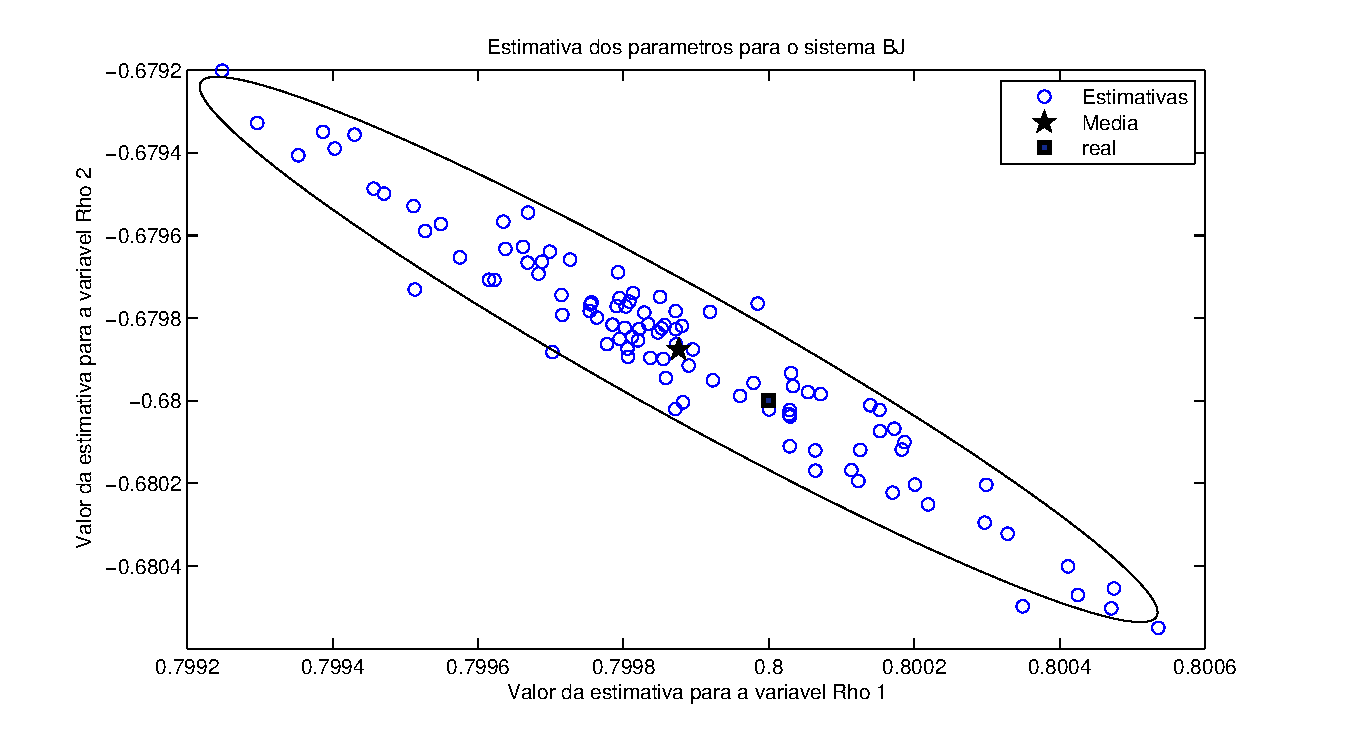
\includegraphics[width=0.95\columnwidth]{figures/vrft_bj_M10_var005.eps}
	\caption{Resultado das 100 estimativas de Monte Carlo dos par�metros $\rho_1$ e $\rho_2$ para o controlador
	apresentado em \eqref{eq:vrft_methos_ex_bj_c}.}
	\label{fig:vrft_bj_M10_var005}
\end{figure}

Os par�metros reais esperados para o controlador (equa��o \eqref{eq:vrft_methos_ex_bj_cd}) e a m�dia de todas
as estimativas (valor representado por uma estrela na Figura (\ref{fig:vrft_bj_M10_var005})) n�o s�o os
mesmos. Em uma situa��o onde o erro de polariza��o das estimativas n�o existe, o aumento de N (n�mero de
amostras) implica que esta diferen�a diminui, tendendo a zero. Em um cen�rio onde h� erro de polariza��o, se 
aumentarmos a vari�ncia do ruido do sistema, ser� observado um aumento desta diferen�a.

Na figura (\ref{fig:vrft_bj_M10_var02}) quadruplicou-se a vari�ncia do ruido inserido no sistema ($\sigma
_\upsilon ^2=0.02$). Observa-se ent�o que o erro de polariza��o existe na estimativa. Como descrito em
\cite{campi_leccini_savaresi2002} quando o m�todo do VRFT � utilizado com ruido nas amostras, a estimativa �
inevitavelmente polarizada. Neste mesmo trabalho � sugerido a utiliza��o de {\it{vari�veis instrumentais}}
(Se��o (\ref{sec:si_par_estim_iv})) para que este erro de polariza��o seja minimizado.

\begin{figure}[htbp] 
	\center 
	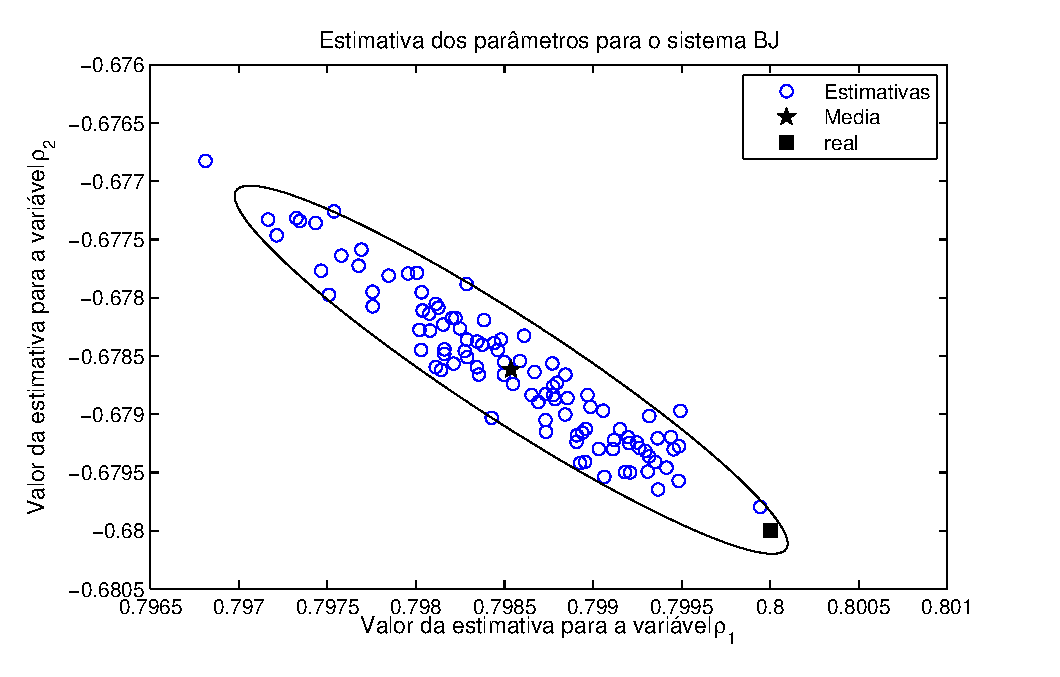
\includegraphics[width=0.95\columnwidth]{figures/vrft_bj_M10_var02.eps}
	\caption{100 estimativas Monte Carlo dos par�metros $\rho_1$ e $\rho_2$ para o controlador apresentado em
	\eqref{eq:vrft_methos_ex_bj_c} com vari�ncia do ruido de 0.02}
	\label{fig:vrft_bj_M10_var02}
\end{figure}

Utilizando o procedimento descrito na se��o (\ref{sec:vrft_framework_noise}) para dados corrompidos por ruido
o resultado obtido, para a mesma vari�ncia de $\sigma_\upsilon ^2=0.02$ do ruido, � apresentado na Figura
(\ref{fig:vrft_bj_M10_var02_iv}).

\begin{figure}[htbp]
	\center
	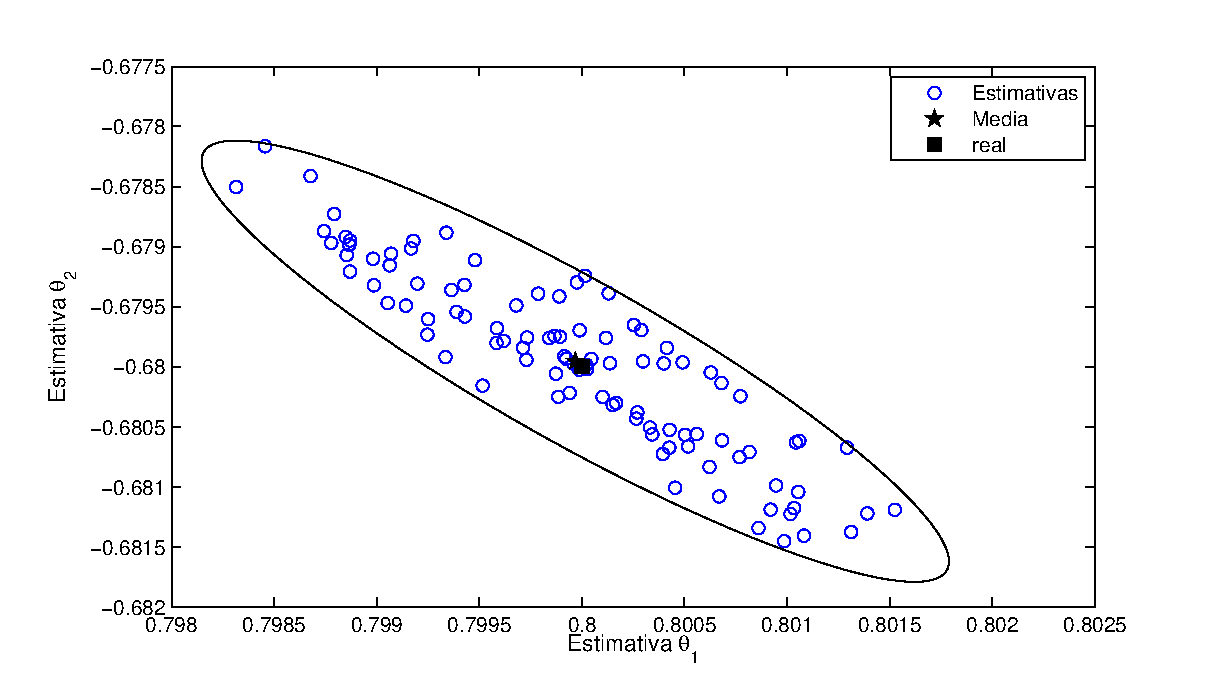
\includegraphics[width=0.95\columnwidth]{figures/vrft_bj_M10_var02_iv.eps}
	\caption{Resultado das 100 estimativas de Monte Carlo dos par�metros $\rho_1$ e $\rho_2$ para o
	controlador apresentado em \eqref{eq:vrft_methos_ex_bj_c} com vari�ncia do
	ruido de 0.02. Utilizando vari�veis instrumentais para estimar os par�metros.}
	\label{fig:vrft_bj_M10_var02_iv}
\end{figure}

Observa-se que o erro de polariza��o foi minimizado e que o resultado obtido possui um custo $J_{VR}^N(\theta)
= 5.1242$ e a vari�ncia dos par�metros estimados foi de $0.5064\times10^{-6}$ para $\rho_1$ e de
$0.5495\times10^{-6}$ para $\rho_2$.

A fim de comparar o m�todo VRFT utilizando e n�o utilizando vari�veis instrumentais s�o apresentados abaixo as
Tabelas (\ref{table:vrft_method_bj}) e (\ref{table:vrft_method_bj_iv}) onde o custo $J_{MR}$ (equa��o
\eqref{eq:vrft_method_cost_func}) e o custo $J_{VR}^N$ (equa��o \eqref{eq:vrft_method_filter_criter_assim})
s�o apresentados para diferentes valores de vari�ncia do ruido para o mesmo sistema BJ.

\begin{table*}[htbp]
\begin{center}
\caption{Valor dos custos $J_{VR}^N$ e $J_{MR}$ al�m da  vari�ncia das
estimativas para diferentes valores de $\sigma _\upsilon ^2$ quando o m�todo
VRFT n�o utiliza vari�veis instrumentais para a estimativa dos par�metros
$\rho$}
\label{table:vrft_method_bj}
\begin{tabular}{cccc}
\hline
        Vari�ncia $\sigma _\upsilon ^2$ & $J_{VR}^N(\theta)$ &
        $J_{MR}(\theta)$ & Vari�ncia estimativas $\rho$   \\
\hline
	    0.06    & 1.7893$\times10^{-2}$ & 8.2367$\times10^{-3}$ & 1.0$\times10^{-5}$\;[0.4754    0.4434] \\
	    0.05    & 1.2515$\times10^{-2}$ & 5.5366$\times10^{-3}$ & 1.0$\times10^{-5}$\;[0.2671    0.3244] \\
        0.04    & 8.1897$\times10^{-3}$ & 3.6071$\times10^{-3}$ & 1.0$\times10^{-5}$\;[0.1534    0.1583] \\
        0.01    & 4.9665$\times10^{-4}$ & 2.4402$\times10^{-4}$ & 1.0$\times10^{-6}$\;[0.0963    0.1035] \\
        0.005   & 1.2515$\times10^{-4}$ & 5.6013$\times10^{-5}$ & 1.0$\times10^{-7}$\;[0.2999    0.3114] \\
        0.001   & 5.0036$\times10^{-6}$ & 3.5734$\times10^{-6}$ & 1.0$\times10^{-8}$\;[0.1301    0.1223] \\
\hline
\end{tabular}
\end{center}
\end{table*} 
   

\begin{table*}[htbp]
\begin{center}
\caption{Valor dos custos $J_{VR}^N$ e $J_{MR}$ al�m da  vari�ncia das
estimativas para diferentes valores de $\sigma _\upsilon ^2$ quando o m�todo
VRFT utiliza vari�veis instrumentais para a estimativa dos par�metros $\rho$}
\label{table:vrft_method_bj_iv}
\begin{tabular}{cccc}
\hline
        Vari�ncia $\sigma _\upsilon ^2$ & $J_{VR}^N(\theta)$ &
        $J_{MR}(\theta)$ & Vari�ncia estimativas $\rho$   \\
\hline
	    0.06    & 45.1719  &  $9.7345\times10^{-5}$ & $1.0\times10^{-5}\;[0.5161    0.5332]$ \\
	    0.05    & 33.2600  &  $2.0457\times10^{-5}$ & $1.0\times10^{-5}\;[0.2481    0.2652]$ \\
        0.04    & 21.2652  &  $1.1665\times10^{-4}$ & $1.0\times10^{-5}\;[0.2040    0.2084]$ \\
        0.01    & 1.2956   &  $8.9695\times10^{-6}$ & $1.0\times10^{-6}\;[0.1246    0.1138]$ \\
        0.005   & 0.3264   &  $7.4764\times10^{-6}$ & $1.0\times10^{-7}\;[0.3063    0.2917]$ \\
        0.001   & 0.0126   &  $5.2443\times10^{-7}$ & $1.0\times10^{-8}\;[0.1059    0.1017]$ \\
\hline
\end{tabular}
\end{center}
\end{table*}

Utilizando vari�veis instrumentais observa-se que o custo $J_{MR}(\theta)$ � significativamente mais baixo
quando comparado com o m�todo onde n�o s�o utilizadas vari�veis instrumentais. Demonstrando assim que o
comportamento desejado do sistema foi atingido com uma melhor aproxima��o.

%===============================================================================
\subsubsection{Controlador PID - sistema ARX}
\label{sec:vrft_examples_pid_arx}
%===============================================================================

Para um sistema {\it{ARX}} onde $G_0(z)$ e $H_0(z)$ podem ser definidos como:

\begin{equation}
G_{ 0 }(z)=\frac { z }{ (z-0.9)(z-0.8) } ,\quad \quad \quad H_{ 0 }(z)=\frac { z^2 }{ (z-0.9)(z-0.8) } 
\nonumber
\end{equation}

Deseja-se que o sistema em malha fechada comporte-se o mais pr�ximo poss�vel do modelo apresentado em:

\begin{equation}
M(z)=\frac { 0.4 }{ z-0.6 }
\label{eq:vrft_methos_ex_arx_M}
\end{equation}

Tem-se assim que o controlador ideal, aquele que ao ser inserido no sistema em
malha fechada apresentado na Figura (\ref{fig:vrft_db_control_loop}) propicia o
comportamento descrito por \eqref{eq:vrft_methos_ex_arx_M} �:

\begin{equation}
C_d(z)=\frac { 0.4(z - 0.9)(z-0.8) }{ z(z-1) }
\label{eq:vrft_methos_ex_arx_cd}
\end{equation}

Observa-se que este controlador pode ser representado como um controlador
{\it{PID}} como em \eqref{eq:vrft_methos_ex_arx_c}. 

\begin{equation}
C(z,\rho )=\frac { \rho _{ 1 }z^2+\rho _{ 2 }z+\rho _{ 3 } }{ z(z-1) } 
\label{eq:vrft_methos_ex_arx_c}
\end{equation}

Na Figura (\ref{fig:vrft_arx_M10_var005}) � apresentado o resultado da estimativa dos par�metros do
controlador quando n�o s�o utilizados vari�veis instrumentais. Obteve-se desta forma um custo
$J_{VR}^N(\theta) = 2.5008\times10^{-5}$ e $J_{MR}(\theta) = 1.7746\times10^{-5}$ al�m de uma vari�ncia para as
estimativas de $1.0\times10^{-7} \; [0.0364\;    0.1261\;    0.0377]$ para $\rho_1$, $\rho_2$ e $\rho_3$
respectivamente.

\begin{figure}[htbp] 
	\center 
	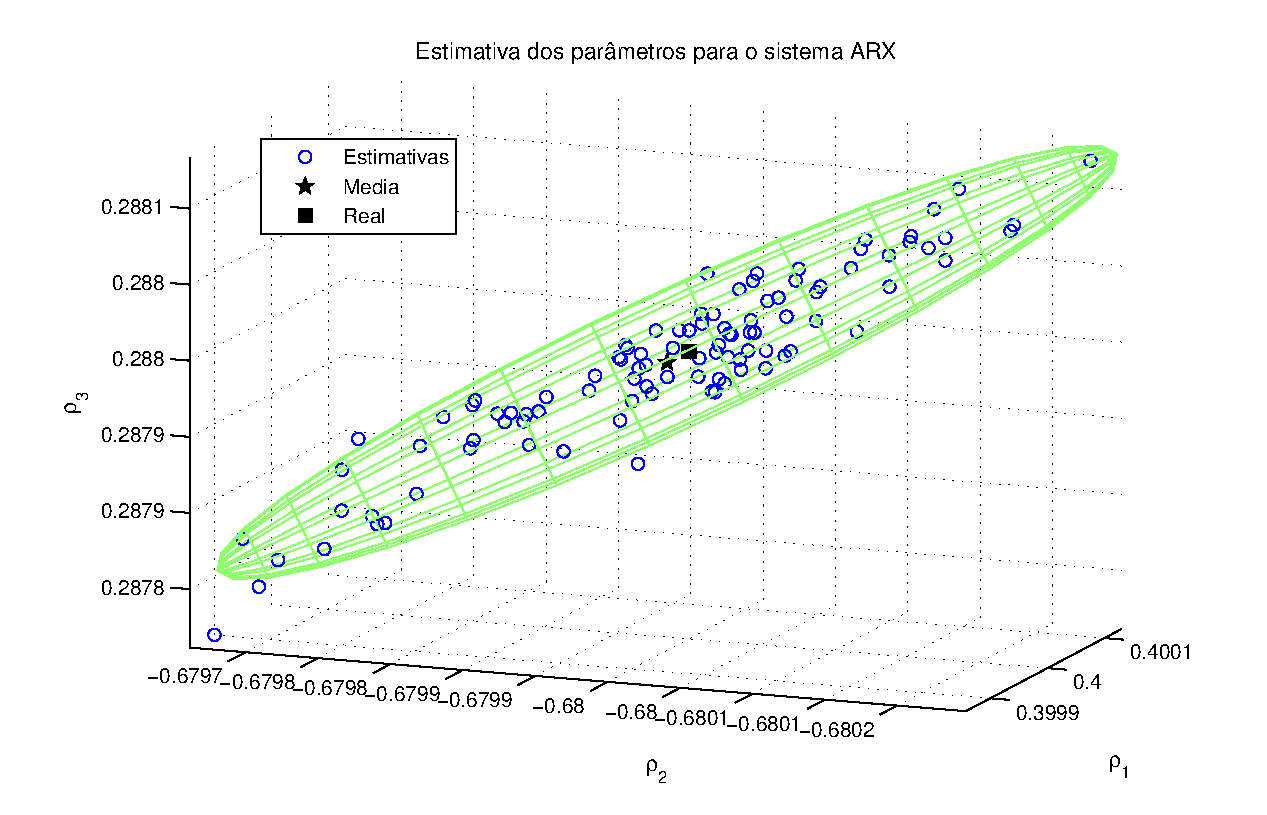
\includegraphics[width=0.95\columnwidth]{figures/vrft_arx_M10_var005_.eps}
	\caption{100 estimativas Monte Carlo dos par�metros $\rho_1$, $\rho_2$ e $\rho_3$ para o controlador
	apresentado em \eqref{eq:vrft_methos_ex_arx_c} com vari�ncia do ruido $\sigma_\upsilon ^2=0.005$}
	\label{fig:vrft_arx_M10_var005}
\end{figure}

Como j� foi observado a utiliza��o de vari�veis instrumentais melhora significativamente o erro de polariza��o existente
nas estimativas. Desta forma as informa��es apresentadas a seguir ser�o feitas utilizando vari�veis instrumentais.
Na figura (\ref{fig:vrft_arx_M10_var05_iv}) � apresentado a estimativa dos par�metros do controlador para um
ruido com vari�ncia $\sigma_\upsilon ^2=0.05$. Observa-se que n�o h� erro de polariza��o nas estimativas. 
O custo para esta, e outas, estimativas � apresentado na Tabela (\ref{table:vrft_method_arx_iv}).

\begin{figure}[htbp] 
	\center 
	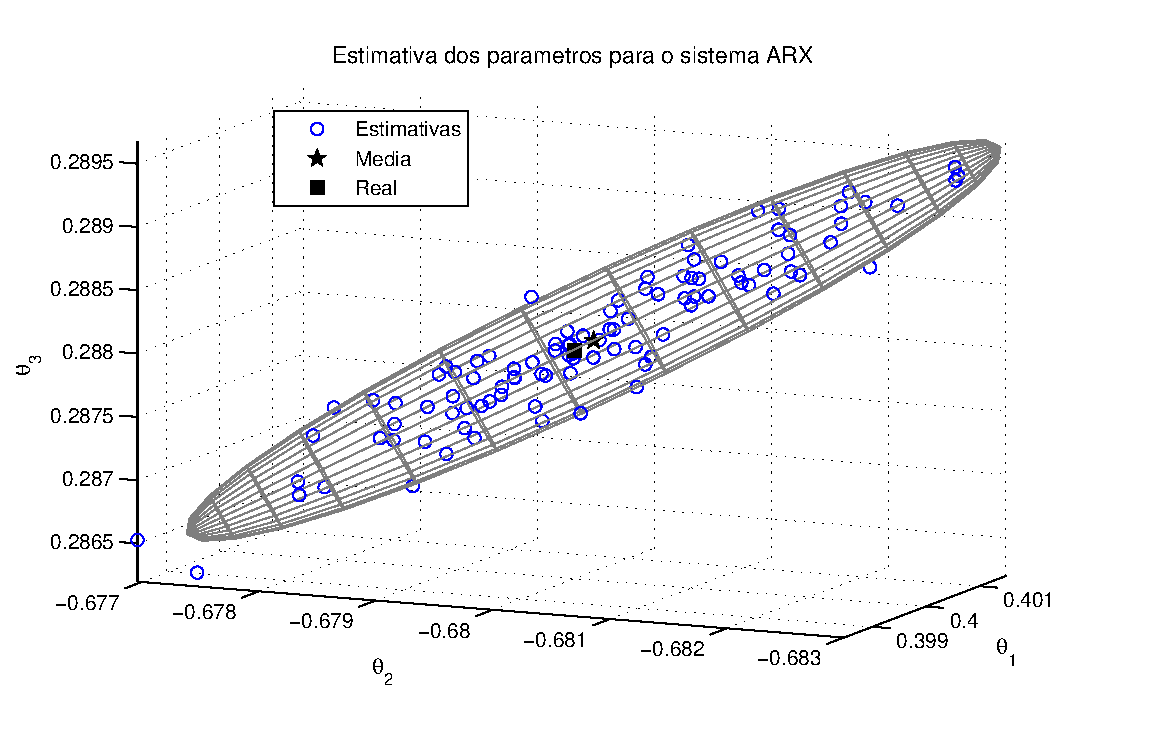
\includegraphics[width=0.95\columnwidth]{figures/vrft_arx_M10_var05_iv.eps}
	\caption{100 estimativas Monte Carlo dos par�metros $\rho_1$, $\rho_2$ e $\rho_3$ para o controlador
	apresentado em \eqref{eq:vrft_methos_ex_arx_c} com vari�ncia do ruido $\sigma_\upsilon ^2=0.05$ utilizando
	vari�veis instrumentais}
	\label{fig:vrft_arx_M10_var05_iv}
\end{figure}


\begin{table*}[htbp]
\begin{center}
\caption{Valor dos custos $J_{VR}^N$ e $J_{MR}$ al�m da  vari�ncia das
estimativas para diferentes valores de $\sigma _\upsilon ^2$ quando o m�todo
VRFT utiliza vari�veis instrumentais para a estimativa dos par�metros $\rho$ do controlador
\eqref{eq:vrft_methos_ex_arx_c}}
\label{table:vrft_method_arx_iv}
\begin{tabular}{cccc}
\hline
        Vari�ncia $\sigma _\upsilon ^2$ & $J_{VR}^N(\theta)$ &
        $J_{MR}(\theta)$ & Vari�ncia estimativas $\rho$   \\
\hline
   0.1     & $10.0743\times10^{-3}$ &  2.2871$\times10^{-3}$ & $1\times10^{-5}\;[0.1253 \; 0.4683 \; 0.1600]$ \\
   0.06    & $ 3.6093\times10^{-3}$ &  1.1279$\times10^{-3}$ & $1\times10^{-5}\;[0.0516 \; 0.1793 \; 0.0575]$ \\
   0.05    & $ 2.5419\times10^{-3}$ &  1.2453$\times10^{-3}$ & $1\times10^{-5}\;[0.0344 \; 0.1237 \; 0.0416]$ \\
   0.04    & $ 1.6013\times10^{-3}$ &  0.5106$\times10^{-3}$ & $1\times10^{-6}\;[0.2195 \; 0.7908 \; 0.2379]$ \\
   0.01    & $10.0077\times10^{-5}$ & 13.7142$\times10^{-5}$ & $1\times10^{-7}\;[0.1552 \; 0.5469 \; 0.1822]$ \\
   0.005   & $ 2.5081\times10^{-5}$ & 10.3482$\times10^{-5}$ & $1\times10^{-7}\;[0.0406 \; 0.1260 \; 0.0375]$ \\
	0.001  & $ 0.1009\times10^{-5}$ &  2.0487$\times10^{-5}$ & $1\times10^{-9}\;[0.1277 \; 0.4035 \;0.1239]$	 \\
\hline
\end{tabular}
\end{center}
\end{table*}

%===============================================================================
\subsubsection{Controlador n�o pertence a classe}
\label{sec:vrft_examples_not_in_class}
%===============================================================================

At� este ponto foram apresentados exemplos de uso do m�todo VRFT quando o controlador que leva o sistema para
o comportamento desejado $M(z)$ faz parte da classe escolhida para a identifica��o. Em outras palavras quando
$C_0(z) \in \mathcal{C(z, \theta)}$. Nesta se��o ser� apresentado um exemplo onde o modelo do controlador escolhido
para o sistema n�o consegue levar este para $M(z)$, ou seja, n�o consegue representar a totalidade das din�micas de
$C_0(z)$.

Considerando o sistema descrito por
\begin{equation}
G_{ 0 }(z)=\frac { 0.2(z-0.7) }{ (z-0.9)(z-0.5) } ,\quad \quad \quad H_{ 0 }(z)=\frac { z }{ z-0.3 } 
\nonumber
\end{equation}

Deseja-se que em malha fechada ele se comporte como em: 

\begin{equation}
M(z)=\frac { 0.16z }{ (z-0.6)^2 }
\label{eq:vrft_methos_ex_pid_not_M}
\end{equation}

Neste caso o controlador ideal � definido por \eqref{eq:vrft_methos_ex_pid_not_cd}

\begin{equation}
C_{ d }(z)=\frac { 0.8z(z-0.9)(z-0.5) }{ (z-1)(z-0.36)(z-0.7) } 
\label{eq:vrft_methos_ex_pid_not_cd}
\end{equation}

Para esta identifica��o optou-se por um controlador do tipo PID como em \eqref{eq:vrft_methos_ex_pid_not_c}
 
\begin{equation}
C(z,\rho )=\frac { \rho _{ 1 }z^2+\rho _{ 2 }z+\rho _{ 3 } }{ z(z-1) } 
\label{eq:vrft_methos_ex_pid_not_c}
\end{equation}

Observa-se que \eqref{eq:vrft_methos_ex_pid_not_c} n�o consegue representar todas as din�micas apresentadas em
\eqref{eq:vrft_methos_ex_pid_not_cd}. Utilizando o procedimento descrito na Se��o
(\ref{sec:vrft_framework_noise}) e o procedimento de experimento repetido, foram feitos 100 experimentos de
Monte Carlo e o resultado obtido para a m�dia das estimativas foi:

\begin{equation}
\rho_L =\left[ 0.8101 \quad -0.1691  \quad -0.3358 \right]
\nonumber
\end{equation}

Onde o �ndice $L$ indica que este resultado foi obtido utilizando-se o filtro $L$.

Repetindo a simula��o, mas agora sem que o procedimento da utiliza��o do filtro $L$ descrito na se��o
(\ref{sec:vrft_framework_noise}), obteve-se o resultado seguinte:

\begin{equation}
\rho =\left[ 0.5846 \quad -0.2108  \quad -0.1525 \right]
\nonumber
\end{equation}

Aplicando-se estes resultados ao controlador apresentado em \eqref{eq:vrft_methos_ex_pid_not_c} e de posse do
comportamento desejado para o sistema em malha fechada ($M(z)$) � poss�vel fazer um comparativo da resposta
ao salto unit�rio para o sistema utilizando os dois controladores obtidos. O resultado � apresentado na Figura
(\ref{fig:vrft_notinclass_step}).

\begin{figure}[htbp] 
	\center 
	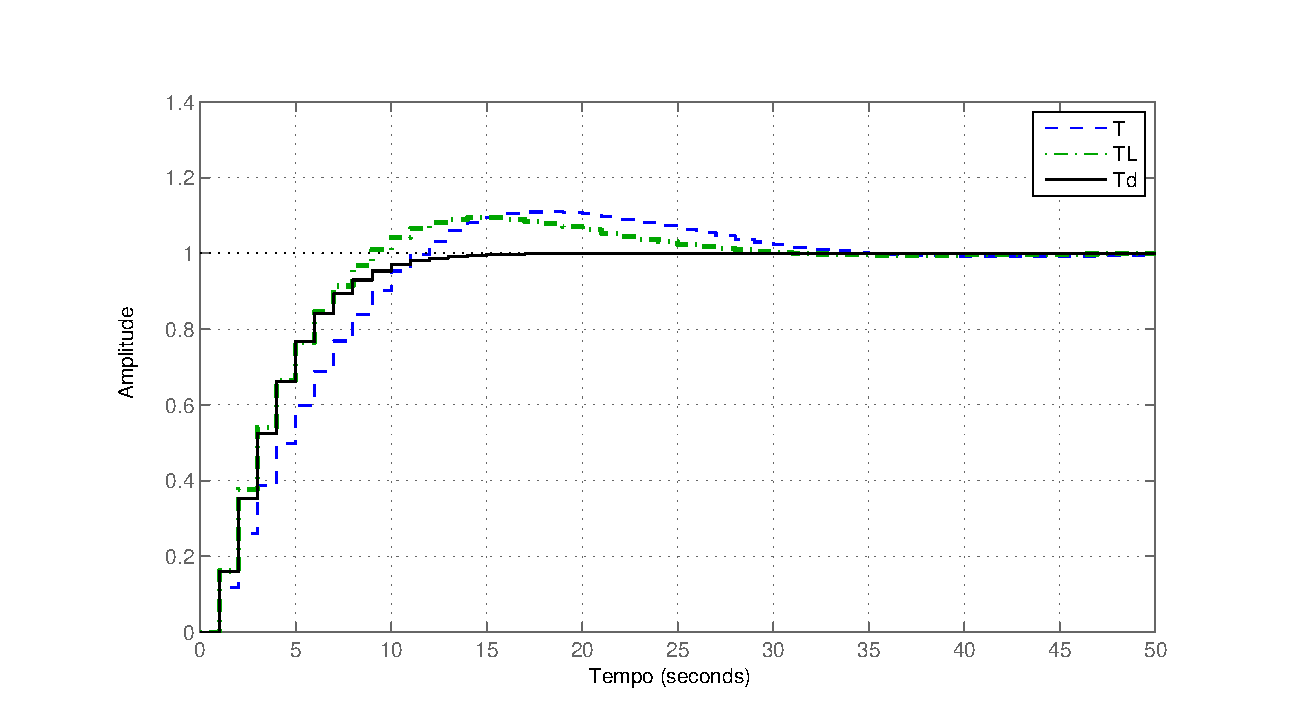
\includegraphics[width=0.95\columnwidth]{figures/vrft_notinclass_step.eps}
	\caption{Comparativo da resposta do sistema a um degrau unit�rio quando o controlador inserido � obtido pelo
	m�todo VRFT utilizando o filtro L e quando n�o se utiliza este artificio. O sistema foi simulado com um
	ruido de vari�ncia $\sigma_\upsilon ^2=0.1$}
	\label{fig:vrft_notinclass_step}
\end{figure}

Observa-se que para o sistema que utiliza o controlador estimado utilizando-se o filtro $L$, a resposta ao
degrau unit�rio tem significativamente menos erro que o sistema utilizando o outro controlador. Ficando este
primeiro muito mais pr�ximo da fun��o $M(z)$ desejada.

Os custos destes dois sistemas � apresentado na Tabela (\ref{table:vrft_method_notinclass}).

\begin{table*}[htbp]
\begin{center}
\caption{Valor dos custos $J_{VR}^N$ e $J_{MR}$ para o sistema controlado por $C(z)$ e $C_L(z)$}
\label{table:vrft_method_notinclass}
\begin{tabular}{ccc}
\hline
        Controlador & $J_{VR}^N(\theta)$ & $J_{MR}(\theta)$ \\
\hline
	$C(z)$   & 0.2877 &  0.1270 \\
	$C_L(z)$ & 0.4481 &  0.0542 \\
\hline
\end{tabular}
\end{center}
\end{table*}

A fim de comparar as duas estimativas, na figura (\ref{fig:vrft_notinclass_bode}) � apresentado o diagrama de
Bode dos controladores obtidos (utilizando a m�dia das estimativas obtidas).

\begin{figure}[htbp] 
	\center 
	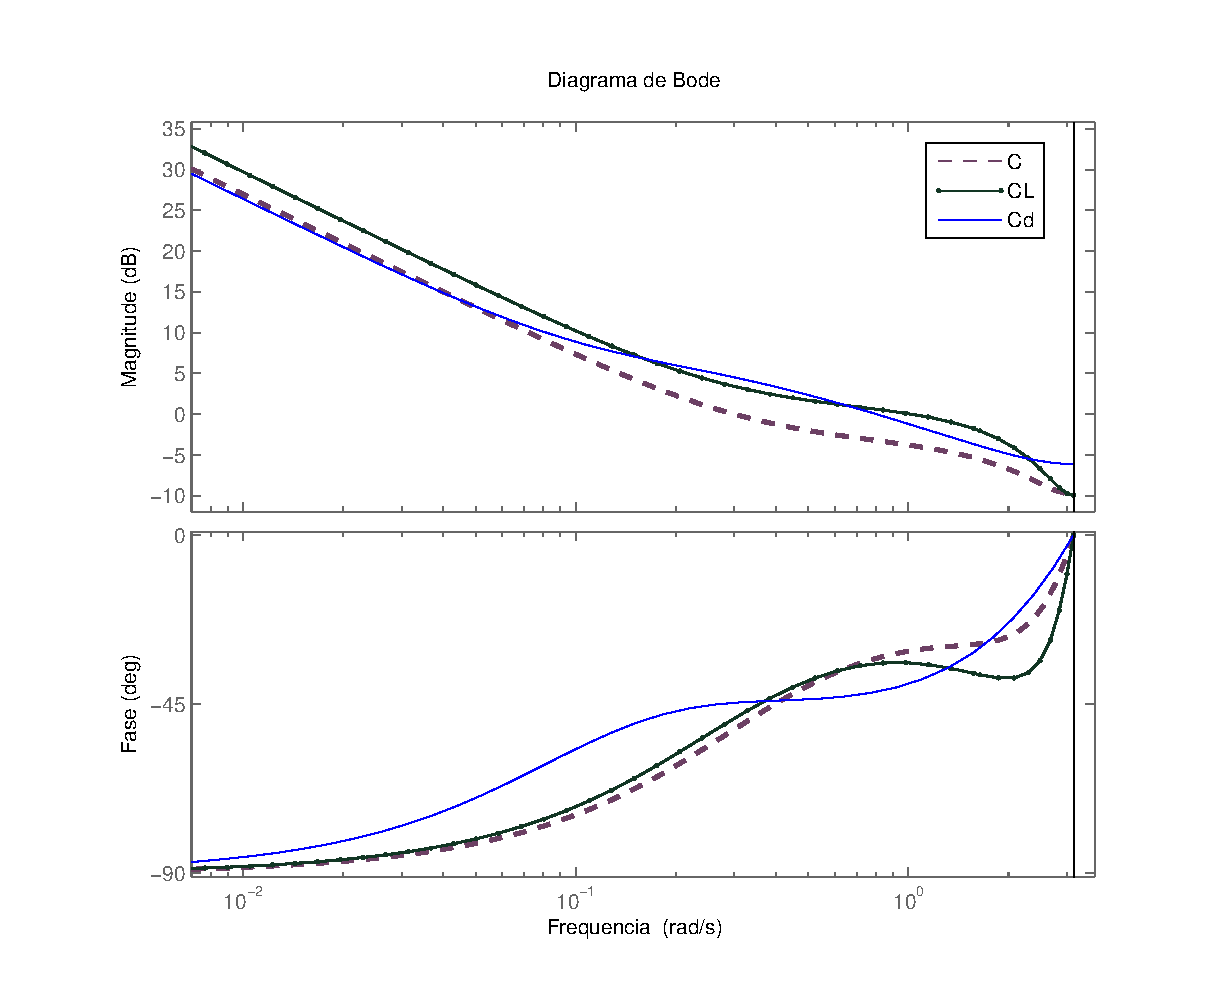
\includegraphics[width=0.99\columnwidth]{figures/vrft_notinclass_bode.eps}
	\caption{Diagrama de Bode para as fun��es de transfer�ncia dos controladores estimados utilizando VRFT com e
	sem o artificio do filtro L e vari�veis instrumentais}
	\label{fig:vrft_notinclass_bode}
\end{figure}


% ===============================================================================
\section{Identifica��o de sistemas n�o lineares utilizando refer�ncia virtual}
\label{sec:vrft_nonlinear}
%===============================================================================

Como visto na se��o \ref{sec:vrft_vrft}, o m�todo VRFT tem um grande apelo, e produz resultados
significativamente satisfat�rios para diversos modelos lineares. 

Nesta se��o o objetivo � demonstrar como este m�todo de comporta com sistemas n�o lineares. Duas
n�o linearidades ser�o apresentadas: est�ticas, para isso ser� utilizado o modelo de Wiener (apresentado na
se��o \ref{sec:nl_models_wiener_hammerstein}) e n�o linearidades din�micas, a classe de modelos escolhido
foram modelos NARMAX racionais (apresentados na se��o \ref{sec:nl_models_narmax_rat}).

A fun��o custo que pretende-se minimizar pode ser expressa como:

\begin{equation}
J(\theta)=\left \| y_{\theta}-M \tilde{r} \right \|^2
\label{eq:vrft_nl_j}
\end{equation} 

Onde $y_{\theta}=G\left [ C_{\theta}\left [ \tilde{r} -D y_{\theta} \right ] \right ]$ e $D$ � o atraso da
planta.

Desta forma o que se observa � que o custo a ser minimizado � dependente da planta que a-priori �
desconhecida. Ent�o � sugerido a minimiza��o de outra fun��o custo que possui a o mesmo minimo que
\eqref{eq:vrft_nl_j}: \cite{campi_savaresi2006}

\begin{equation}
J_{VRFT}(\theta)=\left \| F\left [ C_{\theta}[\tilde{e}] - F[\tilde{u}] \right ] \right \|^2
\label{eq:vrft_nl_jvrft}
\end{equation} 

Onde $F: \mathbb{R}^N\to \mathbb{R}^N$ � um filtro de que deve ser escolhido.

Em \cite{campi_savaresi2006} indica-se a utiliza��o do filtro:

\begin{equation}
F=(I-MD) \left ( \frac{\partial G\left [ u \right ]}{\partial u}|_{\tilde{u}} \right ) 
\label{eq:vrft_nl_filter}
\end{equation} 

Onde $ \frac{\partial G\left [ u \right ]}{\partial u}$ deve ser calculado a partir dos dados coletados.
Imprecis�es nesta estimativa apenas indicam que a segunda derivada de $J_{VRFT}$ n�o ir� precisamente
ter o mesmo m�nimo que $J$. \cite{campi_savaresi2006}

Devido ao custo e dificuldade de se obter $ \frac{\partial G\left [ u \right ]}{\partial u}$ e com o intuito
de utilizar o algoritmo de identifica��o de sistemas racionais apresentados na se��o
\ref{sec:nl_si_algorithms_rationals} optou-se em utilizar sistemas n�o lineares que pudessem ser aproximados
por equa��es n�o lineares racionais ou polinomiais. E desta forma utilizar a metodologia VRFT para gerar os
sinais $\bar{r}(t)$ e $e(t)$, e com isso alimentar o algoritmo de identifica��o de modelos racionais.

Como j� foi discutido, utilizando o m�todo VRFT, pode-se obter os sinais de alimenta��o do controlador, e de
posse do sinal de sa�da deste � poss�vel identificar o controlador que melhor atinge o almejado comportamento
da planta em malha fechada, descrito por $M(z)$.

Desta forma, o que foi alterado do m�todo cl�ssico do VRFT foi a utiliza��o do algoritmo de identifica��o de
modelos racionais, alimentando-o com o sinal de refer�ncia virtual $\bar{r}(t)$ e a sa�da $u(t)$.

A seguir ser�o apresentados alguns exemplos do uso deste procedimento e os resultados obtidos. Os exemplos
ser�o divididos em dois grupos principais: onde existe uma n�o linearidade est�tica na planta, e onde a n�o
linearidade � din�mica.

%===============================================================================
\subsection{N�o linearidades est�ticas}
\label{sec:vrft_nl_wiener}
%===============================================================================

Como n�o linearidade est�tica escolheu-se a classe de modelos de Wiener. Na Figura \ref{fig:vrft_nl_wiener} �
apresentado o diagrama de blocos do sistema, sendo $\Phi$ e $\Phi^{-1}$ os blocos n�o lineares da planta e do
controlador respectivamente.

\begin{figure}[htbp]
\center
% Generated with LaTeXDraw 2.0.8
% Sat May 26 23:30:48 BRT 2012
% \usepackage[usenames,dvipsnames]{pstricks}
% \usepackage{epsfig}
% \usepackage{pst-grad} % For gradients
% \usepackage{pst-plot} % For axes
\scalebox{1} % Change this value to rescale the drawing.
{
\begin{pspicture}(0,-1.32)(11.62,1.3)
\psline[linewidth=0.04cm,arrowsize=0.05291667cm 2.0,arrowlength=1.4,arrowinset=0.4]{->}(0.0,0.3)(0.8,0.3)
\pscircle[linewidth=0.04,dimen=outer](1.0,0.3){0.2}
\psline[linewidth=0.04cm,arrowsize=0.05291667cm 2.0,arrowlength=1.4,arrowinset=0.4]{->}(1.2,0.3)(2.0,0.3)
\psframe[linewidth=0.04,dimen=outer](3.2,0.7)(2.0,-0.1)
\psline[linewidth=0.04cm,arrowsize=0.05291667cm 2.0,arrowlength=1.4,arrowinset=0.4]{->}(3.2,0.3)(4.2,0.3)
\psframe[linewidth=0.04,dimen=outer](5.4,0.7)(4.2,-0.1)
\psframe[linewidth=0.04,dimen=outer](8.0,0.7)(6.8,-0.1)
\psline[linewidth=0.04cm,arrowsize=0.05291667cm 2.0,arrowlength=1.4,arrowinset=0.4]{->}(8.0,0.3)(9.0,0.3)
\psframe[linewidth=0.04,dimen=outer](10.2,0.7)(9.0,-0.1)
\psline[linewidth=0.04cm,arrowsize=0.05291667cm 2.0,arrowlength=1.4,arrowinset=0.4]{->}(5.4,0.3)(6.8,0.3)
\psline[linewidth=0.04cm,arrowsize=0.05291667cm 2.0,arrowlength=1.4,arrowinset=0.4]{->}(10.2,0.3)(11.6,0.3)
\psline[linewidth=0.04cm,arrowsize=0.05291667cm 2.0,arrowlength=1.4,arrowinset=0.4]{<-}(1.0,0.1)(1.0,-1.3)
\psline[linewidth=0.04cm](1.0,-1.3)(10.8,-1.3)
\psline[linewidth=0.04cm](10.8,-1.3)(10.8,0.3)
\usefont{T1}{ppl}{m}{n}
\rput(0.45828125,0.61){r(t)}
\usefont{T1}{ppl}{m}{n}
\rput(1.5445312,0.61){$\epsilon (t)$}
\usefont{T1}{ppl}{m}{n}
\rput(3.699375,0.61){v(t)}
\usefont{T1}{ppl}{m}{n}
\rput(6.089375,0.61){u(t)}
\usefont{T1}{ppl}{m}{n}
\rput(8.464531,0.61){$\omega(t)$}
\usefont{T1}{ppl}{m}{n}
\rput(10.899375,0.61){y(t)}
\psline[linewidth=0.04cm](1.2,0.1)(1.4,0.1)
\psframe[linewidth=0.04,linestyle=dashed,dash=0.16cm 0.16cm,dimen=outer](5.6,1.3)(1.8,-0.3)
\psframe[linewidth=0.04,linestyle=dashed,dash=0.16cm 0.16cm,dimen=outer](10.4,1.3)(6.6,-0.3)
\usefont{T1}{ppl}{m}{n}
\rput(3.5345314,-0.59){C(z)}
\usefont{T1}{ppl}{m}{n}
\rput(8.544531,-0.59){G(z)}
\usefont{T1}{ppl}{m}{n}
\rput(2.5945313,0.29){$\vartheta(t)$}
\usefont{T1}{ppl}{m}{n}
\rput(9.594531,0.31){$\Phi(t)$}
\usefont{T1}{ppl}{m}{n}
\rput(4.7945313,0.31){C'(z)}
\usefont{T1}{ppl}{m}{n}
\rput(7.4045315,0.31){G'(z)}
\usefont{T1}{ppl}{m}{n}
\rput(8.438125,1.01){Wiener}
\usefont{T1}{ppl}{m}{n}
\rput(3.7610939,1.01){Hammerstein}
\end{pspicture} 
}
\caption{Diagrama de blocos para um sistema n�o linear do tipo Wiener}
\label{fig:vrft_nl_wiener}
\end{figure}

Para este exemplo ser�o utilizadas as seguintes defini��es para o sistema:

\begin{equation}
G'(z)=\frac{0.5}{z-0.9}
\label{eq:vrft_nl_wiener_g}
\end{equation} 

$G'(z)$ � a parte linear da planta do sistema. O comportamento do sistema em malha fechada esperado foi
definido como em $M(z)$:

\begin{equation}
M(z)=\frac{0.4}{z-0.6}
\label{eq:vrft_nl_wiener_m}
\end{equation}  

A n�o linearidade presente na planta do sistema foi escolhida como sendo um polin�mio de terceira ordem
descrito como abaixo:

\begin{equation}
\Phi(\omega)=y(t)=1.5\omega(t)+0.2\omega^3(t)
\label{eq:vrft_nl_wiener_phi}
\end{equation}  

Espera-se ent�o que por $M(z)$ ser linear, que o controlador tenha um bloco que seja o inverso de $\Phi$, para
que a n�o linearidade possa ser cancelada completamente.

Atingir uma express�o anal�tica que descreva $\Phi^{-1}$ n�o � uma tarefa simples. Optou-se ent�o por
aproximar esta fun��o por outro polin�mio de ordem 4, definido por $\vartheta (t)$:

\begin{equation}
\vartheta (\epsilon(t))= v(t) = a_1\epsilon (t) + a_2 \epsilon ^2(t) +a_3 \epsilon ^3(t) +a_4 \epsilon ^4(t)
\label{eq:vrft_nl_wiener_phi_inv}
\end{equation}  

Desconsiderando a parte n�o linear presente na planta, � simples de observar que o controlador �timo que
levaria a planta em malha fechada a ter o comportamento descrito por $M(z)$ �:

\begin{equation}
C_d(z)= \frac{0.8z-0.72}{z-1}
\label{eq:vrft_nl_wiener_cd}
\end{equation}  

O controlador $C_d(z)$ possui uma integrador em sua estrutura. Para evitar problemas de seguimento de
refer�ncia optou-se por n�o identificar esta parte do controlador. Mantendo o denominador como um integrador
e identificando apenas o numerador. Juntamente com a identifica��o do controlador da por��o linear $C_d(z)$ �
necess�rio identificar o polin�mio da equa��o \eqref{eq:vrft_nl_wiener_phi_inv}.

Fazendo-se as substitui��es matem�ticas necess�rias, chega-se a express�o do sinal de sa�da do controlador que
se quer identificar:

\begin{equation}
u(t)=\begin{bmatrix}
\theta_1 & \theta_2 & \theta_3 & \theta_4 & \theta_5 & \theta_6 & \theta_7 & \theta_8
\end{bmatrix}
\begin{bmatrix}
\epsilon (t)\\ 
\epsilon ^2(t)\\ 
\epsilon^3(t)\\ 
\epsilon^4(t)\\ 
\epsilon(t-1)\\ 
\epsilon^2(t-1)\\ 
\epsilon^3(t-1)\\ 
\epsilon^4(t-1)
\end{bmatrix}
\label{eq:vrft_nl_wiener_u}
\end{equation}  

Foram feitos 100 experimentos de Monte Carlo e a m�dia das estimativas obtidas foi de:

\begin{equation}
\text{m�dia }\;\theta =\begin{bmatrix}
0.4471 \\ 0.0020 \\ -6.5105\times10^{-4} \\ -1.5959\times10^{-5} \\ -0.4043 \\ -0.0016 \\ 6.1194\times10^{-4}
\\ 1.4562\times10^{-5}
\end{bmatrix}^T
\nonumber
\end{equation}

Com um desvio padr�o de:

\begin{equation}
\text{m�dia }\;\theta = 1\times10^{-3}\begin{bmatrix}
0.2430 \\ 0.0246 \\ 0.0015 \\ 0.0001 \\ 0.2613 \\ 0.0259 \\ 0.0016 \\ 0.0001
\end{bmatrix}^T
\nonumber
\end{equation}

O custo entre os sinais de sa�da do sistema obtido e o sistema esperado $M(z)$ foi de  $J_{MR}(\theta)=
0.3820$ e o custo dos sinais de sa�da do controlador esperado e obtido foi de $J_{VR}=1.0119$.

Como a estimativa de $\vartheta (\epsilon(t))$ � apenas uma aproxima��o do que espera-se ser a inversa de
$\Phi(\omega(t))$, a classe de modelos escolhida para o controlador n�o consegue representar a totalidade do
controlador ideal. Desta forma � esperado que a identifica��o n�o consiga atingir a totalidade da fun��o
$M(z)$ inicialmente escolhido. Para as estimativas foram utilizados sinais PRBS de 127 pontos para a
excita��o da planta.

Na Figura (\ref{fig:vrft_nl_wiener_step}) � apresentado um comparativo entre o sinal de sa�da do sistema
$M(z)$ quando submetido a um degrau unit�rio e o sinal do sistema real quando o controlador identificado �
aplicado sobre a planta em malha fechada.

\begin{figure}[htbp] 
	\center 
	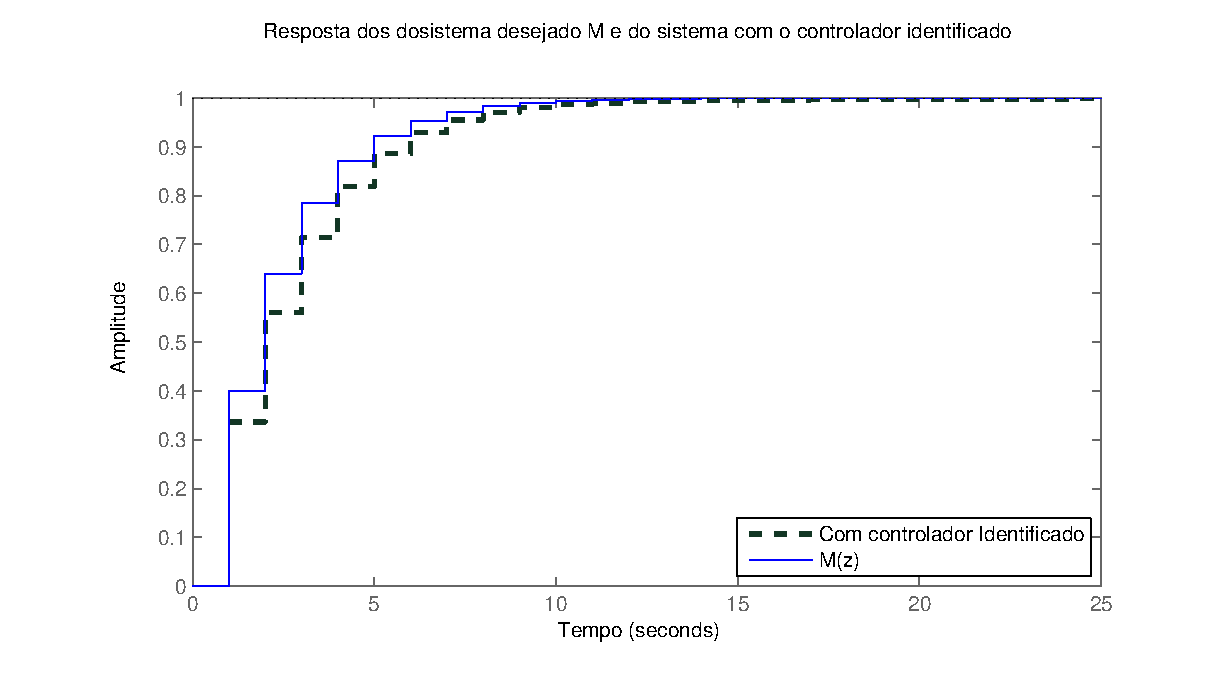
\includegraphics[width=0.95\columnwidth]{figures/vrft_nl_wiener_step.eps}
	\caption{resposta dos sistemas: desejado e obtido a um degrau unit�rio}
	\label{fig:vrft_nl_wiener_step}
\end{figure}

Na Figura (\ref{fig:vrft_nl_wiener_vw_step}) � apresentado o comportamento dos sinais de sa�da e entrada das
n�o linearidades $\Phi^{-1}(e(t))$ e $\Phi(\omega(t))$ respectivamente.

\begin{figure}[htbp] 
	\center 
	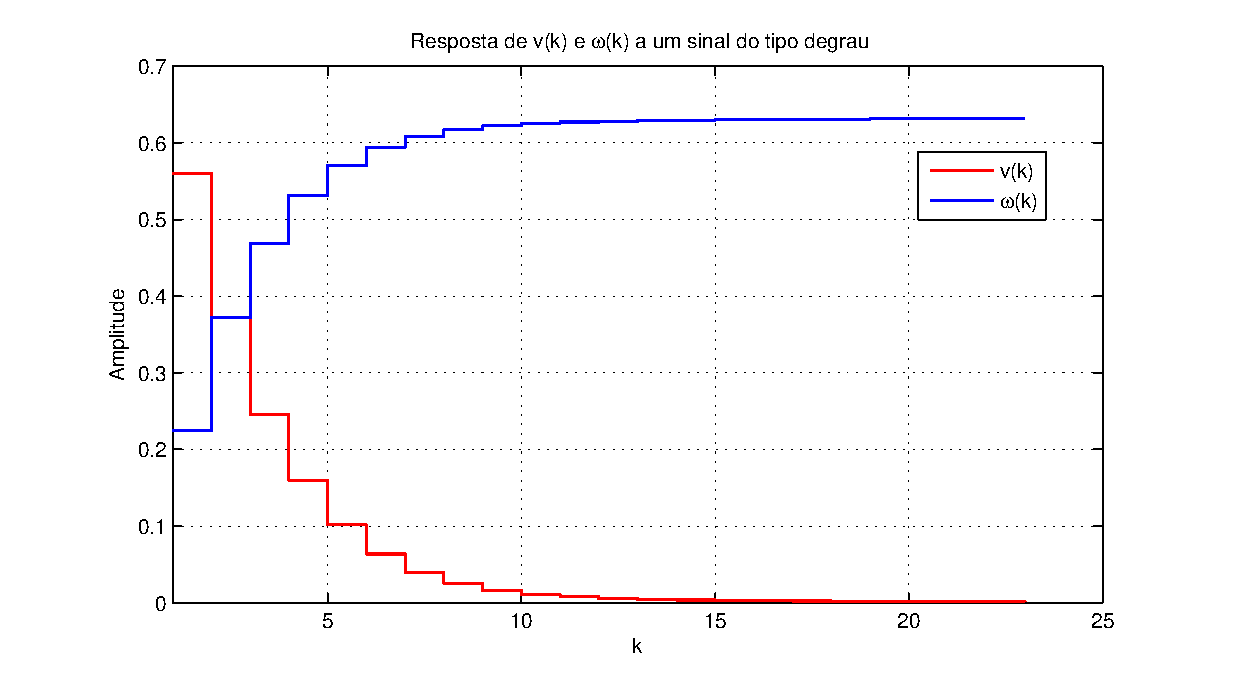
\includegraphics[width=0.95\columnwidth]{figures/vrft_nl_wiener_vw_step.eps}
	\caption{sinais $v(t)$ e $\omega(t)$ quando o sistema � alimentado por um degrau unit�rio}
	\label{fig:vrft_nl_wiener_vw_step}
\end{figure}

A rela��o entre os sinais $v(t)$ e $\omega(t)$ � apresentado na Figura (\ref{fig:vrft_nl_wiener_vw}).
Observa-se que a rela��o destes sinais � praticamente linear, garantido que a aproxima��o de $\Phi^{-1}$ foi
satisfat�ria para representar a inversa do sinal $\Phi$.

\begin{figure}[htbp] 
	\center 
	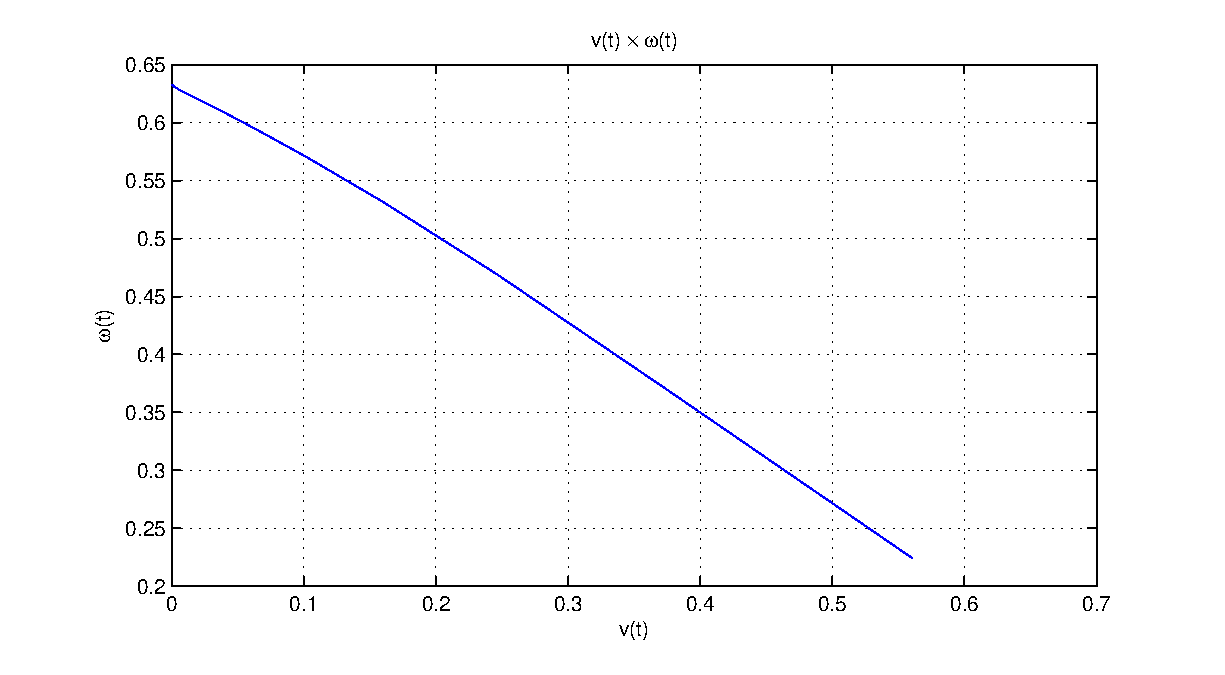
\includegraphics[width=0.95\columnwidth]{figures/vrft_nl_wiener_vw.eps}
	\caption{rela��o entre os sinais $v(t)$ e $\omega(t)$ quando o sistema � alimentado por um degrau unit�rio}
	\label{fig:vrft_nl_wiener_vw}
\end{figure}

%===============================================================================
\subsection{N�o linearidades din�micas}
\label{sec:vrft_nl_dinamic}
%===============================================================================
Nesta se��o ser�o apresentados alguns exemplos do algoritmo apresentado na Se��o
\ref{sec:nl_si_algorithms_rationals} em conjunto com o principio b�sico do m�todo VRFT para a obten��o dos
sinais $r(t)$ e $e(t)$, al�m do sinal escolhido $u(t)$ utilizado para excitar a planta e o pr�prio sinal de
sa�da da planta $y(t)$.

\TODO: escrever algo mais aqui !!!!!!

%===============================================================================
\subsubsection{Controlador sendo representado pelo modelo}
\label{sec:vrft_nl_dinamic_c_match}
%===============================================================================

Considere a planta descrita por:

\begin{equation}
y(t)=\frac{0.1u(t-1)y(t-1)+u(t-1)}{1+0.25y^2(t-2)}
\label{eq:vrft_nl_dinamic_ex1_y}
\end{equation}

Deseja-se que em malha fechada seu comportamento seja como em:

\begin{equation}
M(z)=\frac{Y(z)}{R(z)}=\frac{0.4}{z-0.6}
\label{eq:vrft_nl_dinamic_ex1_mz}
\end{equation}

A equa��o de $M(z)$ pode ser reescrita em fun��o do tempo como em:

\begin{equation}
y(t)=0.4r(t-1)+0.6y(t-1)
\label{eq:vrft_nl_dinamic_ex1_mt}
\end{equation}

Ao igualarmos a equa��o \eqref{eq:vrft_nl_dinamic_ex1_y} com \eqref{eq:vrft_nl_dinamic_ex1_mt} e isolando o
sinal $u(t)$ temos a equa��o que descreve o comportamento do controlador que levar� a planta a ter o
comportamento descrito por $M(z)$ em malha fechada. Obt�m-se desta forma um controlador ideal como em:

\begin{equation}
u(t)=\frac{0.4r(t)+0.6y(t)+0.1y^2(t-2)r(t-1)+0.15y(t)y^2(t-1)}{1+0.5y(t)}
\label{eq:vrft_nl_dinamic_ex1_cd}
\end{equation}

Escolhendo um conjunto de modelos que consegue representar o controlador �timo:

\begin{equation}
u(t)=\frac{\theta_1 r(t)+ \theta_2 y(t)+ \theta_3 y^2(t-2)r(t-1)+ \theta_4 y(t)y^2(t-1)}{1+ \theta_5 y(t)}
\label{eq:vrft_nl_dinamic_ex1_c}
\end{equation}

Utilizando um sinal PRBS de tamanho 254 e o m�todo do VRFT para gerar os sinais $r(t)$ e $e(t)$. 
Adicionando-se um ruido de vari�ncia $\sigma^2 = 0.005$, a m�dia da estimativa para 100 experimentos de
Monte Carlo foi de:


\begin{equation}
\text{m�dia de }\theta=\begin{bmatrix}
0.4000 & 0.5999 & 0.1001 & 0.1501 & 0.5000
\end{bmatrix}
\nonumber
\end{equation}

\begin{equation}
\text{Desvio padr�o de }\theta=1.0\times 10^{-3}\begin{bmatrix}
0.2231 & 0.6866 & 0.2411 & 0.6817 & 0.3019
\end{bmatrix}
\nonumber
\end{equation}

\begin{equation}
\text{Covari�ncia }\theta=1.0\times 10^{-6}\begin{bmatrix}
 0.0498 &  0.0585 & -0.0353 & -0.0362 & -0.0018 \\
 0.0585 &  0.4714 & -0.0449 & -0.3690 &  0.0057 \\
-0.0353 & -0.0449 &  0.0581 &  0.0745 & -0.0040 \\
-0.0362 & -0.3690 &  0.0745 &  0.4647 & -0.0070 \\
-0.0018 &  0.0057 & -0.0040 & -0.0070 &  0.0911
\end{bmatrix}
\nonumber
\end{equation}

Simulando o sistema obtido com o controlador estimado e o sistema em malha fechada desejado, o erro observado
� apresentado na figura \ref{fig:vrft_nl_dynamic_step_erro}.

\begin{figure}[htbp] 
	\center 
	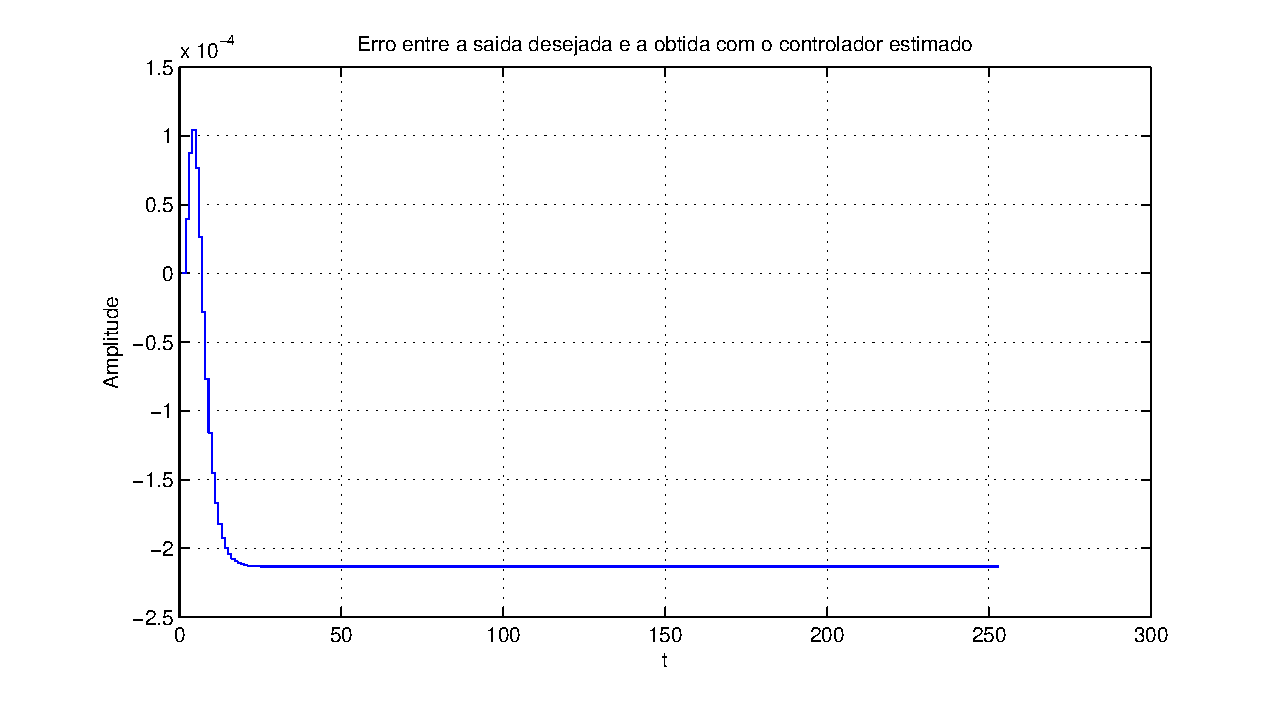
\includegraphics[width=0.95\columnwidth]{figures/vrft_nl_dynamic_erro_step.eps}
	\caption{Erro entre o a resposta esperada e obtida para uma entrada do tipo degrau unit�rio}
	\label{fig:vrft_nl_dynamic_step_erro}
\end{figure}

E a fim de ilustrar as estimativas obtidas pelo m�todo, na Figura \ref{fig:vrft_nl_dynamic_t1_t2} s�o
apresentados as estimativas para os 100 experimentos realizados, al�m da elipse de confian�a de $\chi^2=95\%$
para os parametros $\theta_1$ e $\theta_2$.

\begin{figure}[htbp] 
	\center 
	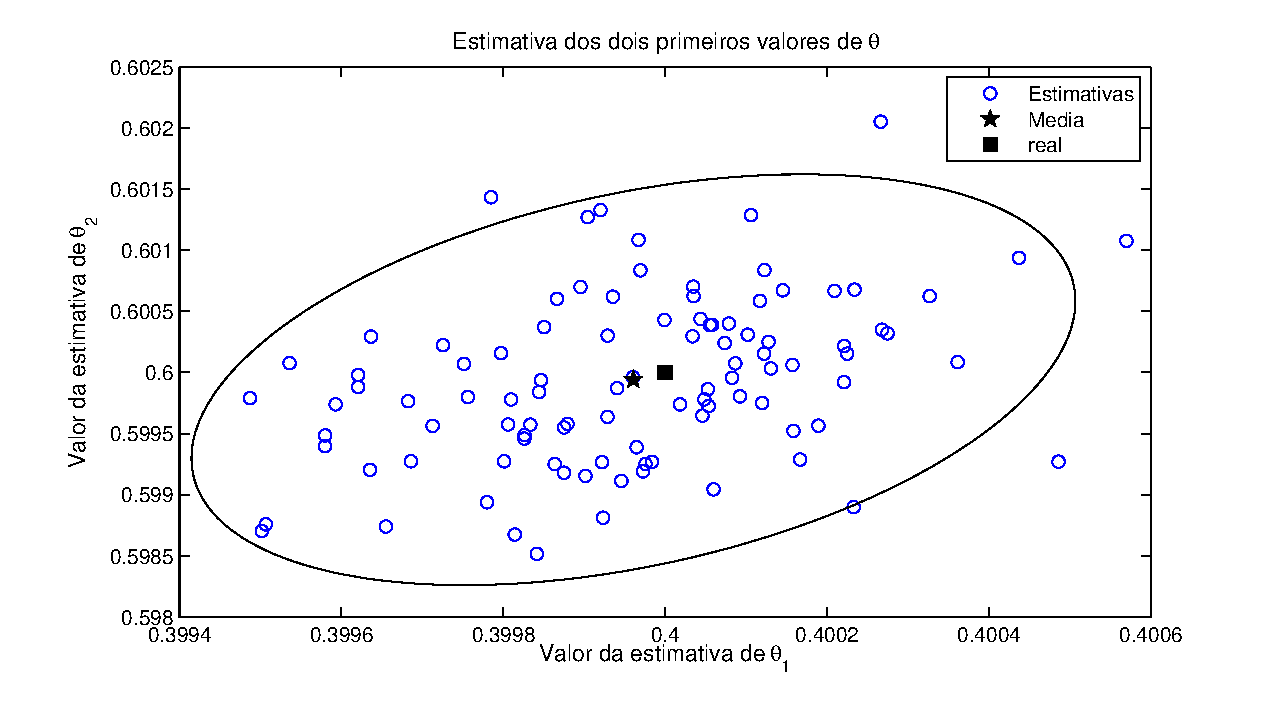
\includegraphics[width=0.95\columnwidth]{figures/vrft_nl_dynamic_t1_t2.eps}
	\caption{100 esperimentos de Monte Carlo das vari�veis $\theta_1$ e $\theta_2$}
	\label{fig:vrft_nl_dynamic_t1_t2}
\end{figure}

O custo $J_{VRFT}=2.7291\times10{-8}$ foi obtido utilizando-se os sinais de sa�da do controlador obtido e
esperado. J� o custo entre os sinais de sa�da do sistema em malha fechada estimado e desejado foi de
$J_{MR}=0.0033$.


\cite{lecchini_campi_savaresi_2dof}
\cite{Guardabassi}



%ruido de 0.01
%
%mtheta =
%
%    0.4000    0.5997    0.1000    0.1503    0.5007
%
%
%vartheta =
%
%   1.0e-04 *
%
%    0.0609    0.6407    0.0593    0.4256    0.0970
%
%
%stdtheta =
%
%    0.0025    0.0080    0.0024    0.0065    0.0031
%
%
%covtheta =
%
%   1.0e-04 *
%
%    0.0609    0.1062   -0.0435   -0.0642   -0.0062
%    0.1062    0.6407   -0.0792   -0.4292    0.0071
%   -0.0435   -0.0792    0.0593    0.0902   -0.0097
%   -0.0642   -0.4292    0.0902    0.4256   -0.0194
%   -0.0062    0.0071   -0.0097   -0.0194    0.0970
%
%
%Jvr_nl =
%
%   1.9177e-06
%
%
%Jmr_nl =
%
%    0.0148
%
%===============================================================================
\subsubsection{Controlador sendo representado pelo modelo 2}
\label{sec:vrft_nl_dinamic_c_match2}
%===============================================================================

%===============================================================================
\subsubsection{Controlador n�o sendo representado pelo modelo}
\label{sec:vrft_nl_dinamic_c_not_match}
%===============================================================================








































%===============================================================================
\section{Considera��es Finais}
\label{sec:vrft_conclusions}
%===============================================================================


%===============================================================================


%===============================================================================
\chapter{Conclus�o}
\label{chapter:conclusion}
%===============================================================================

Neste trabalho diversos assuntos foram abordados para que fosse poss�vel chegar � proposta de projeto de
controladores n�o lineares utilizando refer�ncia virtual. Iniciou-se pela teoria b�sica de identifica��o de sistemas
lineares no Cap�tulo \ref{chapter:system_identification} onde foram apresentados os componentes principais
que permeiam toda a teoria de identifica��o. Foram apresentados alguns dos principais m�todos de identifica��o e quais
s�o suas particularidades e propriedades estat�sticas das estimativas obtidas.

No Capitulo \ref{chapter:nlin_si_ident} foram apresentados as principais classes de modelos para representar sistemas
n�o lineares. Deu-se um enfoque maior para a classe de modelos NARMAX com a apresenta��o do algoritmo de identifica��o
proposto para esta classe de modelos. Exemplos de uso foram apresentados e o que ficou evidenciado � o algoritmo �
bastante eficiente ao que ele se prop�em. Existe entretanto alguns pontos que podem ser tratados como trabalhos
futuros: a converg�ncia do algoritmo est� atrelada a converg�ncia do modelos do ru�do. Nos exemplos estudados o ru�do
aplicado foi pouco representativo para fazer com que houvesse qualquer diverg�ncia de converg�ncia do algoritmo, mas em
situa��es onde a classe de modelos n�o consegue representar todas as din�micas do sistema real ($\mathcal{S} \notin
\mathcal{M}$) o erro de polariza��o das estimativas era esperado, mas se um modelo de ru�do mais complexo fosse
adicionado, a percep��o que se tem � que este erro seria reduzido e com isso uma melhor estimativa poderia ser obtida.
Como nestes exemplos o escopo era apenas demonstrar o funcionamento do algoritmo em situa��es onde o conhecimento da
planta � limitado e que o modelo escolhido n�o � subdimensionado, n�o se investiu no desenvolvimento desta melhoria para
o algoritmo.

Classes de modelos NARMAX possuem alguns diferenciais que os destacam de outras classes de modelos para sistemas n�o
lineares: este tipo de classe consegue representar uma grande quantidade de sistemas reais pois relaciona tanto os
sinais passados da entrada, sa�da e do ru�do do sistema, al�m de que podem ser organizados de uma forma polinomial ou
racional, aumentando a possibilidades de combina��es de classes formadas. Outro ponto de destaque � que este tipo de
classe � parametriz�vel linearmente, isso torna o algoritmo de identifica��o mais simples al�m de assegurar v�rias
propriedades estat�sticas das estimativas feitas para sistemas lineares.

No Cap�tulo \ref{chapter:dbcd} foi apresentada a ideia b�sica para projetos de controladores baseados em dados. Foram
presentados brevemente alguns dos principais m�todos existentes. O m�todo VRFT foi mais detalhado e alguns exemplos de
uso do m�todo foram apresentados. Resultados
obtidos para os exemplos apresentados foram satisfat�rios, observou-se que o m�todo em sua concep��o original possui
erro de polariza��o quando os dados est�o corrompidos por ruido, mesmo que este seja branco. Com a proposta de uso de
vari�veis instrumentais, mostrou-se que este erro de polariza��o desaparece, ampliando os horizontes de utiliza��o da
metodologia.

No Cap�tulo \ref{chapter:dbnarmax} os resultados centrais deste trabalho foram apresentados. Uniu-se a ideia de
refer�ncia virtual com o algoritmo de identifica��o de sistemas n�o lineares descritos por classe de modelos NARMAX
apresentado no Capitulo \ref{chapter:nlin_si_ident}. Para esta situa��o, o sistema a ser identificado pelo algoritmo � o
controlador que � projetado baseado nas necessidades de desempenho do sistema em malha fechada, determinadas pelo
projetista.

Um controlador n�o linear tipicamente ser� requerido quando a planta tiver comportamento n�o linear, mas o comportamento
do sistema em malha fechada desejado for linear. Desta forma o controlador ser� encarregado, al�m de cumprir os
requisitos de desempenho do sistema, de cancelar as n�o linearidades presentes na planta. A escolha de um comportamento
linear em malha fechada normalmente � o caso para o m�todo VRFT e neste trabalho todos os exemplos seguiram esta
caracter�stica.

A escolha de um comportamento n�o linear para o sistema em malha fechada pode ser o caso de alguma aplica��o, mas neste
trabalho n�o foi abordado, poderia entretanto, ser tratado como trabalho futuro, visto que algumas suposi��es para o uso de
refer�ncia virtual devam ser modificadas para cobrir esta situa��o e gerar os sinais necess�rios para a identifica��o.

Os exemplos apresentados para sistemas com n�o linearidades est�ticas e com n�o linearidades na din�mica do processo
apresentados no Cap�tulo \ref{chapter:dbnarmax} mostraram-se bem completas e em conjunto com situa��es onde o
controlador ideal n�o consegue ser representado pela classe de modelos ($\mathcal{S} \notin \mathcal{M}$), cobriram
grande parte das situa��es comumente encontradas na pr�tica.

Desta forma � poss�vel afirmar que a metodologia proposta � v�lida e o est�gio atual de desenvolvimento propicia o uso
desta metodologia em aplica��es pr�ticas.


% \chapter{Estado da arte}
% \chapter{Mais estado da arte}
% \chapter{A minha contribui��o}
% \chapter{Prova de que a minha contribui��o � v�lida}
% \chapter{Conclus�o}

% referencias
% Aqui pode ser usado o ambiente padrao `thebibliography'; por�m, fa�a um
% favor a s� mesmo e use o \bibtex\ e o estilo abnt.bst (veja na p�gina do
% UTUG). 

\bibliographystyle{abnt}

%\bibliography{exemplo,modelo} 	% pode-se ter v�rios arquivos .bib separados
\bibliography{neuhaus} 	% pode-se ter v�rios arquivos .bib separados
				% por v�rgulas. Segundo a NBR6023, as
				% refer�ncias devem ser alinhadas apenas a
				% esquerda. � esquisito, mas � assim.

% Ap�ndices
\appendix

% Pode-se ter diversos ap�ndices
\chapter{T�tulo do Ap�ndice}

Nos ap�ndices aparecem textos ou documentos elaborados pelo autor  a fim de
complementar sua argumenta��o sem preju�zo do trabalho. Eles sempre dever�o
estar depois das refer�ncias e antes dos anexos.


% Anexos
\annex

% Pode-se ter diversos anexos
\chapter{T�tulo do Anexo}

J� os anexos ser�o textos, trabalhos e materiais que n�o foram elaborados
pelo autor, mas que servem de comprova��o, fundamenta��o ou ilustra��o dos
argumentos contidos no texto. Neste ponto, deve-se dar especial aten��o �
quest�o dos direitos autorais.

\end{document}
